\documentclass[12pt,a4paper]{article}
\usepackage[utf8]{inputenc}
\usepackage[margin=1in]{geometry}
\usepackage{graphicx}
\usepackage{float}
\usepackage{amsmath}
\usepackage{booktabs}
\usepackage{caption}
\usepackage{subcaption}
\usepackage{listings}
\usepackage{xcolor}
\usepackage{enumitem}
\usepackage{indentfirst}
\usepackage{hyperref}

\hypersetup{
    colorlinks=true,
    linkcolor=blue,
    filecolor=magenta,      
    urlcolor=cyan,
}

\title{Parking Detection Using Deep Learning}
\author{
    Francis Cho\\
    Hitakshi Chugh\\
    Sugakabiyrarosha\\
    Alvis Chi Hin Ngan\\
    John Allan Ellingson
}
\date{December 3, 2025}

\begin{document}

\maketitle

\newpage
\tableofcontents
\newpage
\listoffigures
\newpage
\listoftables

\newpage
\section{Introduction}

Parking space detection is a critical component of intelligent transportation systems and smart city infrastructure. With the increasing urbanization and the growing number of vehicles, efficient parking management has become essential. This project addresses the challenge of automatically detecting and classifying parking spaces using deep learning techniques.

\subsection{Problem Statement}

The primary objective of this project is to develop and compare multiple deep learning models for parking space detection and classification. The system should be able to:
\begin{itemize}
    \item Detect parking spaces in images
    \item Classify each detected space into one of three categories: free, occupied, or partially occupied
    \item Provide real-time or near-real-time inference capabilities
    \item Achieve high accuracy while maintaining reasonable computational efficiency
\end{itemize}

This problem has significant real-world applications including:
\begin{itemize}
    \item Smart parking management systems
    \item Automated parking guidance systems
    \item Traffic flow optimization
    \item Urban planning and infrastructure development
\end{itemize}

\subsection{Dataset}

The project utilizes multiple datasets across different phases:

\textbf{Phase 1 Datasets:}

\textbf{1. Roboflow Parking Lot Dataset:}
\begin{itemize}
    \item Format: YOLO format
    \item Classes: \texttt{empty}, \texttt{occupied}
    \item Total images: 1,066 images
    \item Split: 936 train, 120 validation, 10 test
    \item Pre-processing: Auto-orientation, resize to 416x416
    \item Augmentations: Horizontal flip (50\%), vertical flip (50\%), rotation (-45° to +45°)
\end{itemize}

\textbf{2. HuggingFace Parking Space Detection Dataset:}
\begin{itemize}
    \item Format: XML annotations (converted to YOLO format)
    \item Classes: \texttt{free\_parking\_space}, \texttt{not\_free\_parking\_space}, \texttt{partially\_free\_parking\_space}
    \item Structure: Contains bounding box annotations for parking spaces
\end{itemize}

\textbf{Phase 1.5 Dataset: PKLot Dataset}
\begin{itemize}
    \item Source: PKLot parking lot dataset
    \item Parking Lots: UFPR04, UFPR05, PUCPR
    \item Weather Conditions: Sunny, Cloudy, Rainy
    \item Structure: Images organized by date, weather condition, and parking lot
    \item Processing: Images aligned using template matching, bounding boxes detected using YOLOv8n, parking spaces identified through clustering
    \item Output: Training data with labeled parking spaces (occupied/free) across multiple dates
    \item Training Samples: 56,602 samples generated from clustered parking spaces (48,111 train, 8,491 validation)
    \item Key Feature: Clustering approach identifies stable parking space locations across temporal sequences
    \item SAM Training: Used for fine-tuning Segment Anything Model (SAM) with two-stage approach for parking space segmentation
\end{itemize}

\textbf{Phase 1 Dataset Summary:}
\begin{itemize}
    \item Total images: 30 images (limited dataset for initial experimentation)
    \item Roboflow dataset: 936 train, 120 validation, 10 test images
    \item HuggingFace dataset: Converted to YOLO format with 3 classes
    \item Purpose: Model development, architecture comparison, and baseline establishment
    \item Class distribution (validation set): Free (89), Not Free (143), Partially Free (1) - significant imbalance
\end{itemize}

The Phase 1 dataset was processed and converted to a unified YOLO format with three classes:
\begin{enumerate}
    \item \texttt{free\_parking\_space}
    \item \texttt{not\_free\_parking\_space}
    \item \texttt{partially\_free\_parking\_space}
\end{enumerate}

\subsection{Phase 2: Augmented Dataset}

Phase 2 introduces a significantly expanded dataset created through data augmentation techniques applied to the PKLot dataset. This section describes the augmentation methodology and dataset characteristics.

\subsubsection{Source Dataset}

The Phase 2 dataset is based on the PKLot parking lot dataset, obtained directly from the university's website\footnote{PKLot dataset: \url{https://web.inf.ufpr.br/vri/databases/parking-lot-database/}}.

\textbf{Dataset Citation:}
\begin{itemize}
    \item Almeida, P., Oliveira, L. S., Silva Jr, E., Britto Jr, A., Koerich, A., PKLot – A robust dataset for parking lot classification, Expert Systems with Applications, 42(11):4937-4949, 2015.
\end{itemize}

\textbf{Dataset Characteristics:}
\begin{itemize}
    \item \textbf{Total Images:} 12,417 images
    \item \textbf{Parking Lots:} Three different parking lots (UFPR04, UFPR05, PUCPR)
    \item \textbf{Weather Conditions:} Images cover different weather conditions and time-of-day variations
    \item \textbf{Format:} Original images with XML annotations containing irregular quadrilateral bounding boxes
\end{itemize}

\textbf{Augmented Dataset:}
The final augmented dataset is available at: \url{https://georgebrowncollege-my.sharepoint.com/:f:/g/personal/101598907_georgebrown_ca/Ej-m50i362BAjtWJSbZJkroBKIvOhYTE0K9e2XwzvYEbeA?e=dXPfN9}

\subsubsection{Augmentation Methodology}

The augmented dataset was created using the PKLot parking lot dataset as the source. The augmentation process (implemented in \texttt{P2\_00\_5\_parking\_augment.py}) addresses several challenges with the original dataset:

\textbf{1. Dataset Limitations:}
\begin{itemize}
    \item The original PKLot dataset is not ready for training as-is
    \item Parking spots outside the labeled region (blue box) are not annotated (see Figure~\ref{fig:dataset_augmentation_pklot_original})
    \item To avoid overfitting, images are cropped to the blue box region, discarding unlabeled data
    \item The original dataset uses irregular quadrilaterals as bounding boxes, which do not follow parking spot markings nor vehicles accurately
\end{itemize}

\textbf{2. Image Preprocessing:}
\begin{itemize}
    \item \textbf{Cropping:} Each parking lot has a predefined crop region (blue box) to focus on the parking area:
    \begin{itemize}
        \item UFPR04: (200, 0, 1100, 720)
        \item UFPR05: (80, 30, 1200, 720)
        \item PUCPR: (300, 180, 1200, 600)
    \end{itemize}
    \item \textbf{Bounding Box Conversion:} Irregular quadrilaterals are converted to vertical rectangular bounding boxes described by center location, width, and height. This maintains consistency with Phase 1 of the project.
    \item \textbf{Resizing:} All images resized to 640×640 pixels (standard for object detection models)
    \item \textbf{Coordinate Transformation:} Bounding box coordinates adjusted for cropping and resizing
\end{itemize}

\textbf{3. Augmentation Pipeline:}
The PKLot dataset only consists of three camera angles (one for each parking lot). To reduce the likelihood of overfitting, we augment the dataset by applying the following augmentation techniques at random using the Albumentations library:

\begin{itemize}
    \item \textbf{Rotation:} ±45 degrees - helps model handle different camera angles
    \item \textbf{Random Brightness and Contrast:} Simulates different lighting conditions
    \item \textbf{Hue-Saturation-Value (HSV) Adjustments:} Hue shift ±10°, saturation ±20, value ±10 (p=0.5) - handles color variations
    \item \textbf{Gaussian Noise:} Variance 10-50 (p=0.3) - adds robustness to sensor noise
    \item \textbf{Gaussian Blur:} Blur limit 3-5 (p=0.3) - simulates motion blur or focus issues
\end{itemize}

\textbf{4. Augmentation Strategy:}
\begin{itemize}
    \item \textbf{Number of Augmentations:} 3 versions per original image (1 original + 2 augmented)
    \item \textbf{Bounding Box Preservation:} All augmentations properly transform bounding box coordinates
    \item \textbf{Validation:} Invalid bounding boxes (outside image bounds, too small) are filtered out
    \item \textbf{Format:} Output saved as JSON annotations with Pascal VOC bbox format [x\_min, y\_min, x\_max, y\_max]
\end{itemize}

\subsubsection{Phase 2 Dataset Statistics}

The Phase 2 augmented dataset provides a substantial increase in data volume:

\textbf{Dataset Overview:}
\begin{itemize}
    \item \textbf{Total Images:} 36,426 images (expanded from 12,417 original PKLot images)
    \item \textbf{Image Size:} 640×640 pixels
    \item \textbf{Annotation Format:} JSON (Pascal VOC bbox format)
    \item \textbf{Classes:} 2 classes (free\_parking\_space, not\_free\_parking\_space)
    \item \textbf{Augmentations per Original:} 3 (1 original + 2 augmented versions)
    \item \textbf{Expansion Factor:} ~2.93× increase from original dataset
\end{itemize}

\textbf{Class Distribution (from 1,000 sample analysis):}
\begin{itemize}
    \item \textbf{Total Parking Spaces Analyzed:} 88,699 spaces
    \item \textbf{Free Spaces:} 30,172 (34.0\%)
    \item \textbf{Occupied Spaces:} 58,527 (66.0\%)
    \item \textbf{Average Spaces per Image:} 88.70
    \item \textbf{Average Occupied Ratio:} 0.660
\end{itemize}

\textbf{Bounding Box Statistics (from 44,396 boxes analyzed):}
\begin{itemize}
    \item \textbf{Mean Width:} 32.39 pixels (std: 8.13)
    \item \textbf{Mean Height:} 79.79 pixels (std: 13.78)
    \item \textbf{Mean Area:} 2,639.94 pixels²
    \item \textbf{Mean Aspect Ratio:} 0.411 (width/height)
    \item \textbf{Range:} Width 3-57px, Height 20-120px
\end{itemize}

\textbf{Key Differences from Phase 1:}
\begin{itemize}
    \item \textbf{Scale:} 36,426 images vs. 30 images (1,214× increase)
    \item \textbf{Format:} JSON annotations vs. YOLO TXT format
    \item \textbf{Classes:} 2 classes (free/occupied) vs. 3 classes (free/occupied/partial)
    \item \textbf{Source:} PKLot dataset vs. Roboflow + HuggingFace
    \item \textbf{Augmentation:} Systematic augmentation applied vs. minimal augmentation
\end{itemize}

Table~\ref{tab:phase_comparison} provides a direct comparison between Phase 1 and Phase 2 datasets.

\begin{table}[H]
\centering
\caption{Phase 1 vs. Phase 2 Dataset Comparison}
\label{tab:phase_comparison}
\begin{tabular}{@{}lcc@{}}
\toprule
\textbf{Characteristic} & \textbf{Phase 1} & \textbf{Phase 2} \\
\midrule
Total Images & 30 & 36,426 \\
Image Size & Variable & 640×640 \\
Annotation Format & YOLO (TXT) & JSON (Pascal VOC) \\
Number of Classes & 3 & 2 \\
Classes & free, not\_free, partial & free, occupied \\
Source Dataset & Roboflow + HuggingFace & PKLot \\
Augmentation & Minimal & Systematic (3× per image) \\
Avg. Spaces/Image & ~7.7 & 88.70 \\
Class Distribution & Highly imbalanced & More balanced \\
\bottomrule
\end{tabular}
\end{table}

Figure~\ref{fig:phase2_stats} shows the distribution of parking spaces, occupied ratios, and augmentation indices in the Phase 2 dataset.

\begin{figure}[H]
\centering
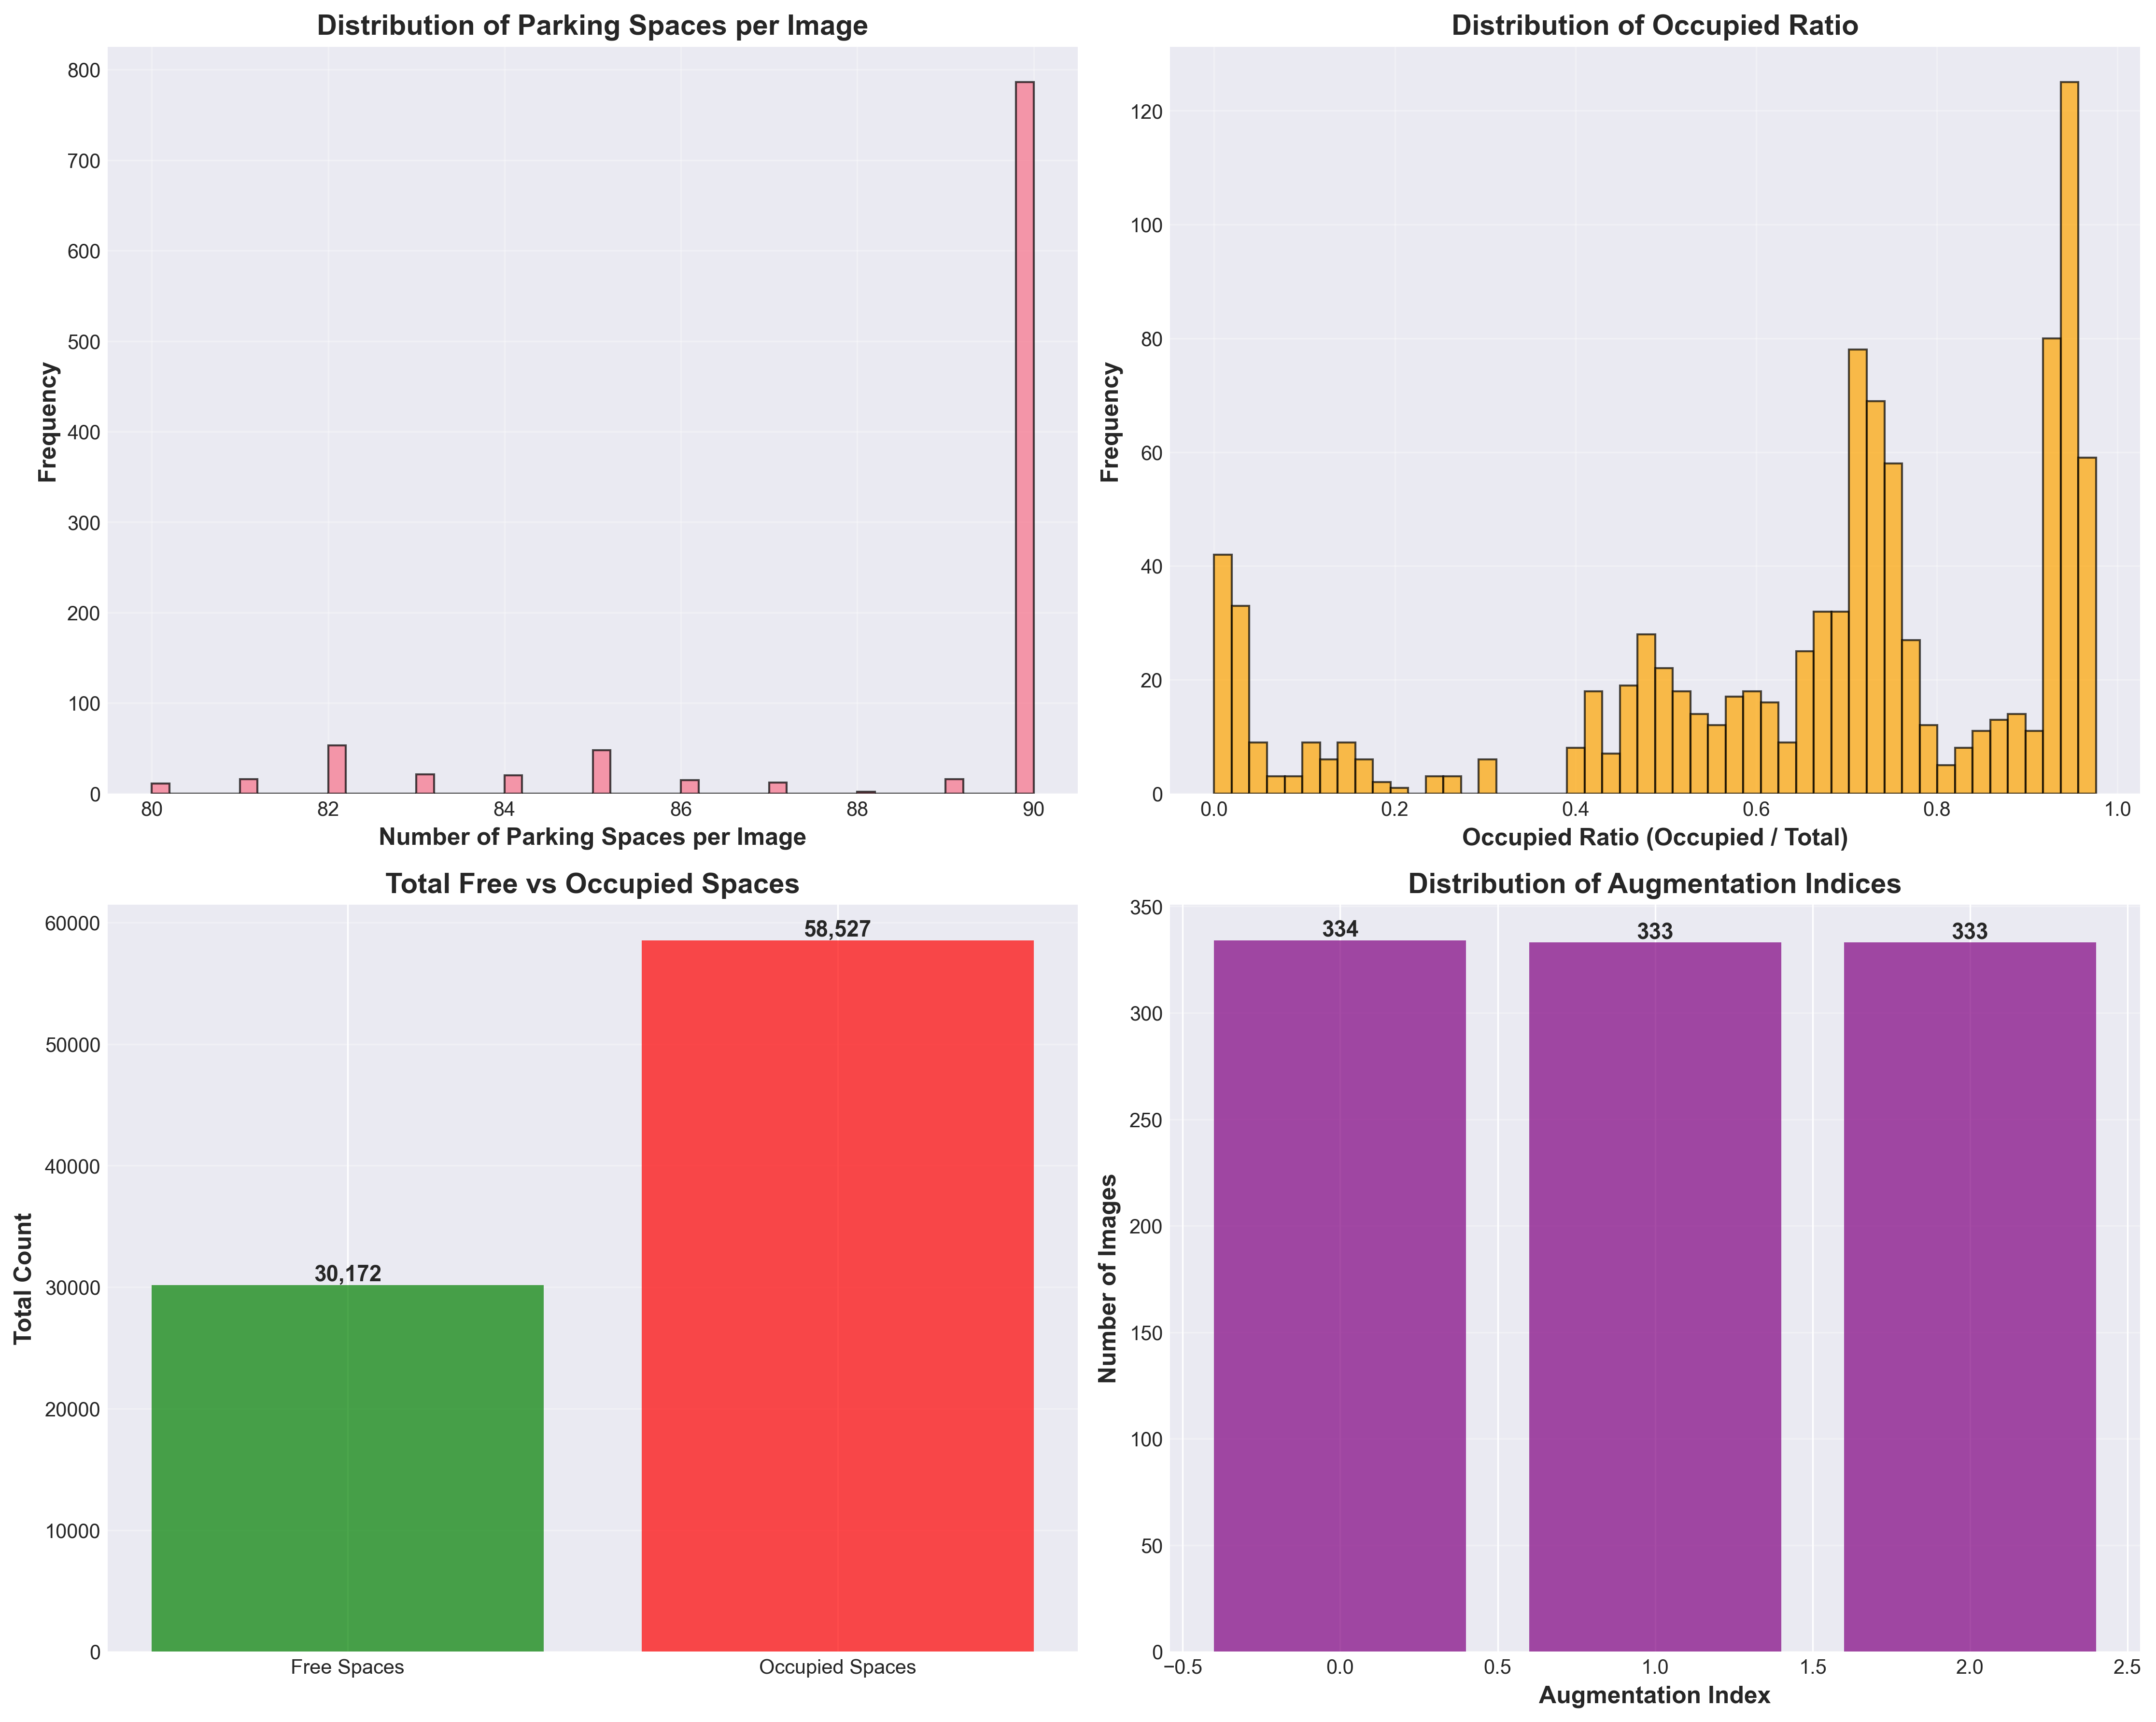
\includegraphics[width=0.9\textwidth]{temp/phase2_statistics.png}
\caption{Phase 2 Dataset Statistics: Distribution of parking spaces per image, occupied ratio, class distribution, and augmentation indices}
\label{fig:phase2_stats}
\end{figure}

Figure~\ref{fig:phase2_samples} shows sample images from the augmented dataset with bounding box annotations.

\begin{figure}[H]
\centering
\includegraphics[width=0.9\textwidth]{temp/phase2_sample_images.png}
\caption{Phase 2 Sample Images: Random samples with bounding box annotations (Green=Free, Red=Occupied)}
\label{fig:phase2_samples}
\end{figure}

Figure~\ref{fig:phase2_bbox} shows the distribution of bounding box dimensions and aspect ratios.

\begin{figure}[H]
\centering
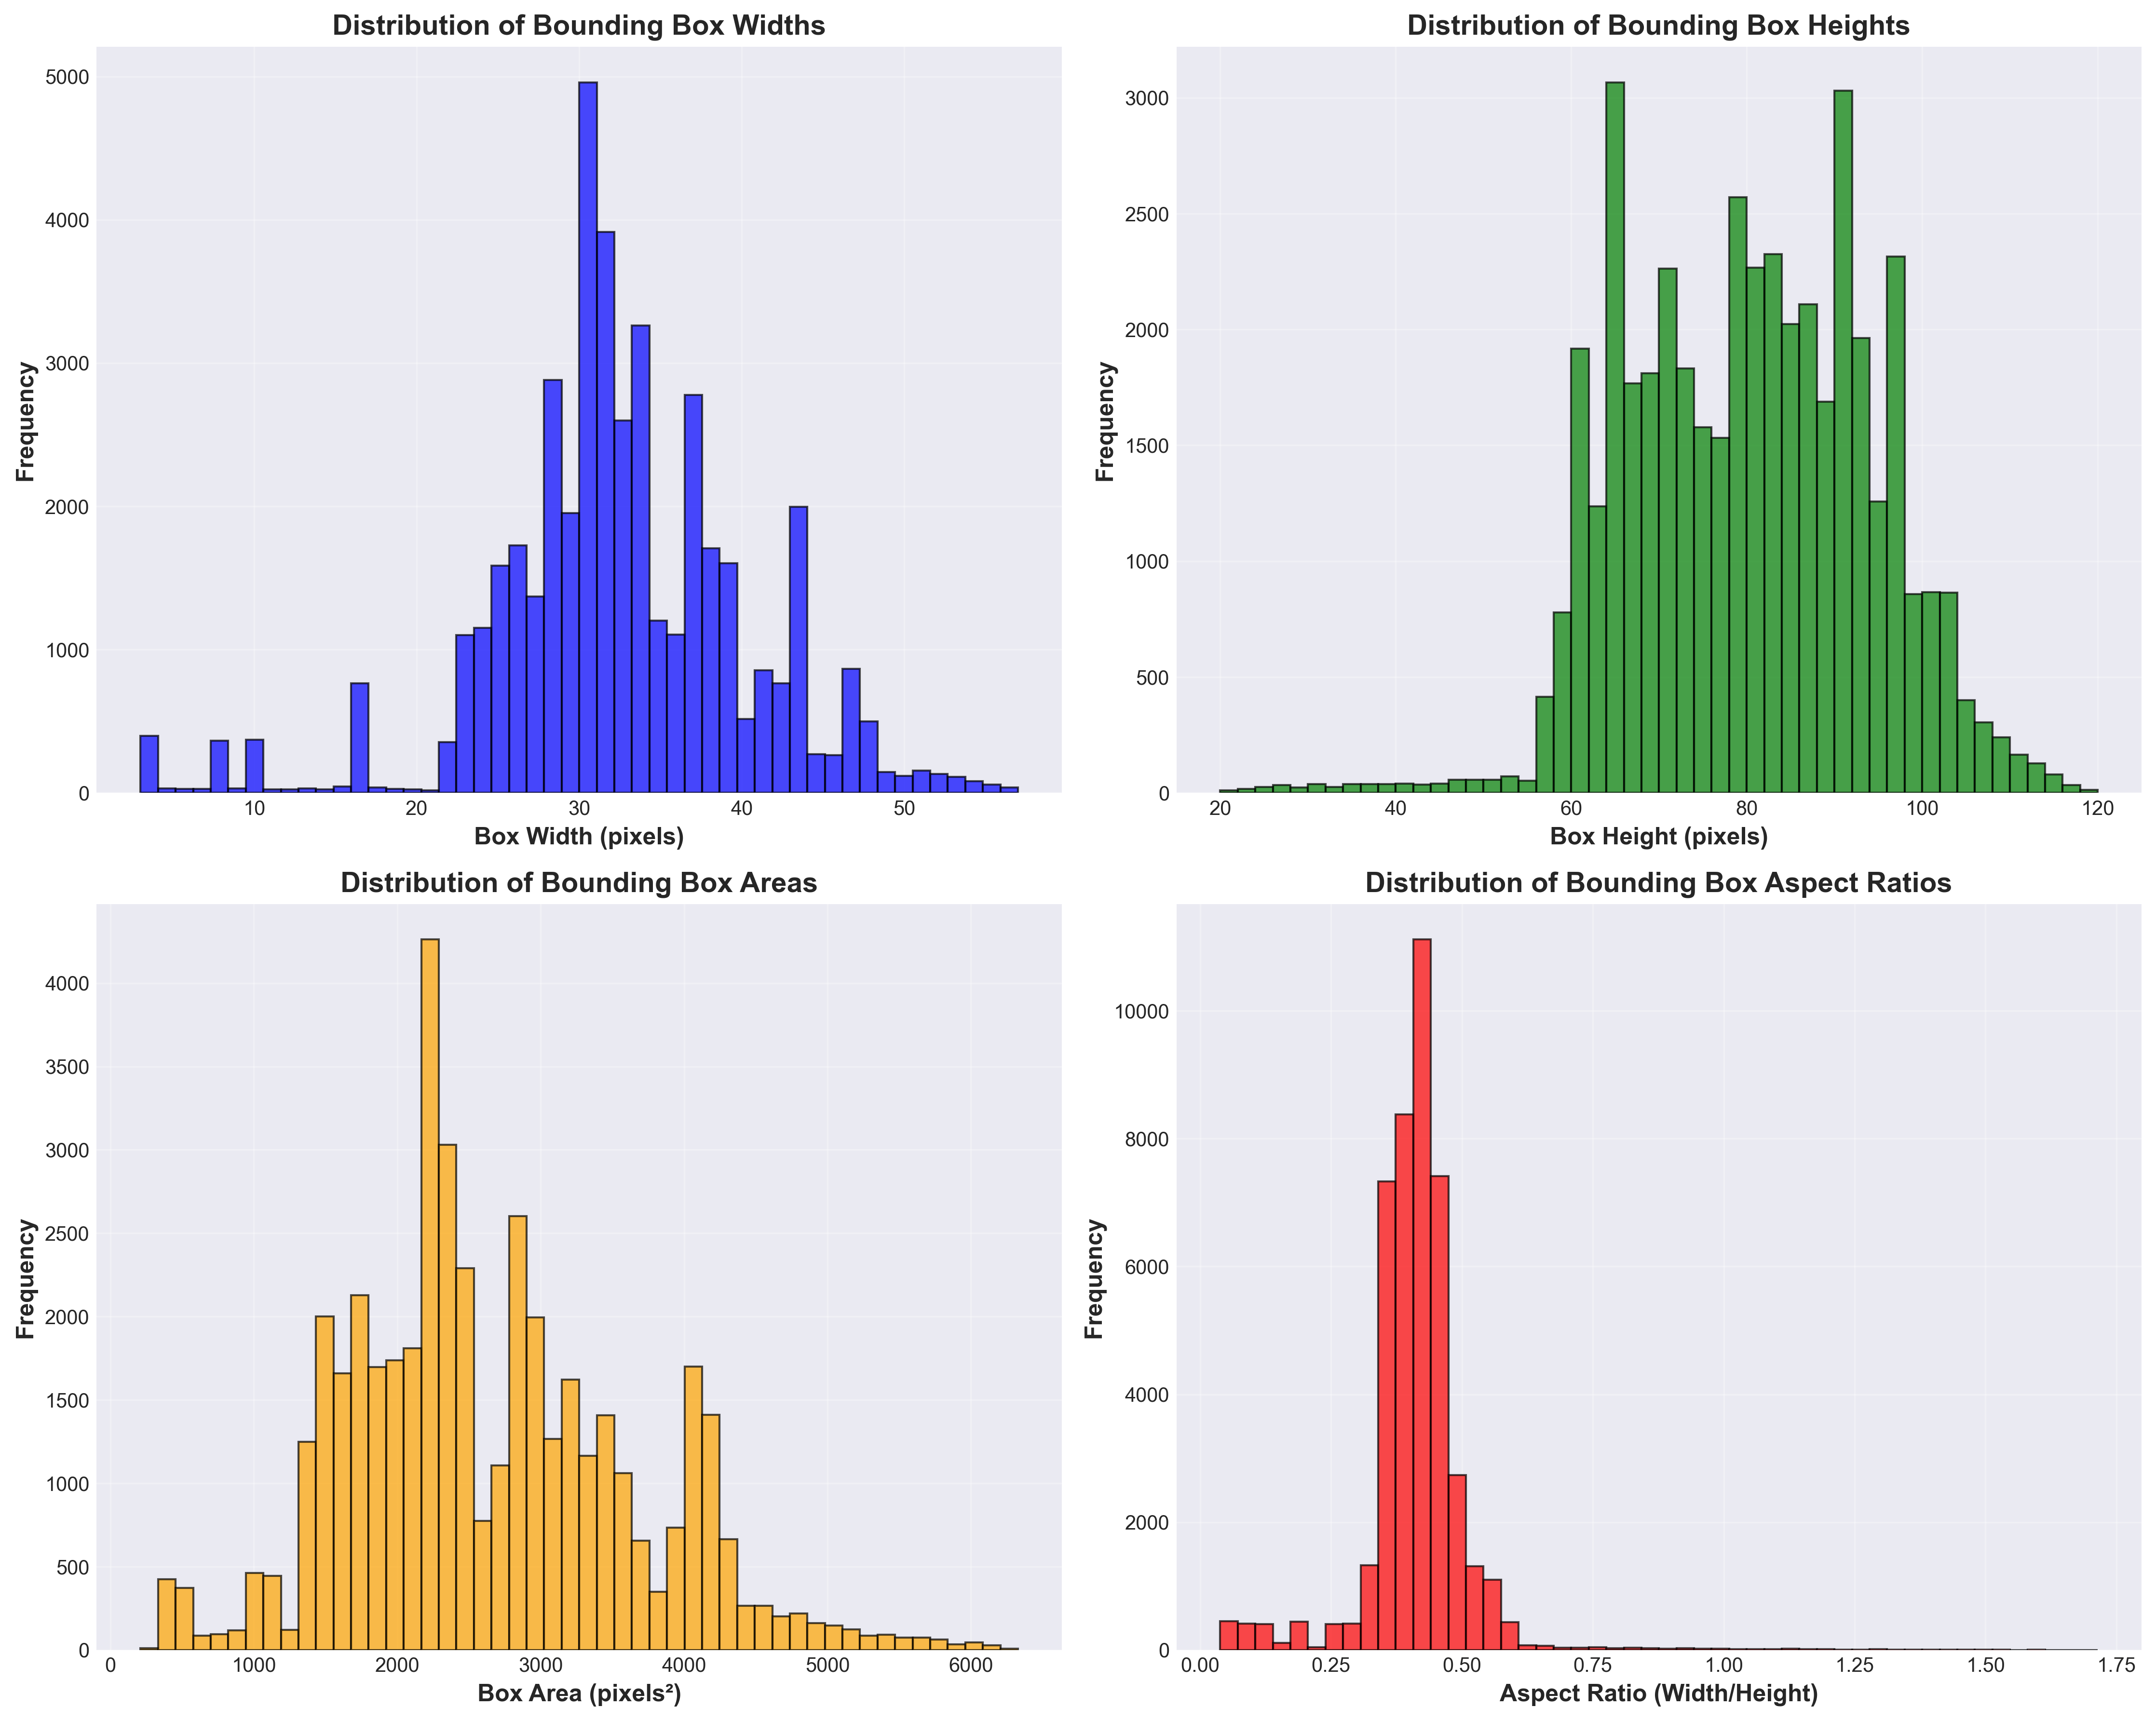
\includegraphics[width=0.9\textwidth]{temp/phase2_bbox_statistics.png}
\caption{Phase 2 Bounding Box Statistics: Distribution of widths, heights, areas, and aspect ratios}
\label{fig:phase2_bbox}
\end{figure}

Figure~\ref{fig:dataset_augmentation_pklot_original} shows an example of the original PKLot dataset image, demonstrating the blue box crop region and the irregular quadrilateral bounding boxes that were converted to rectangular format.

\begin{figure}[H]
\centering
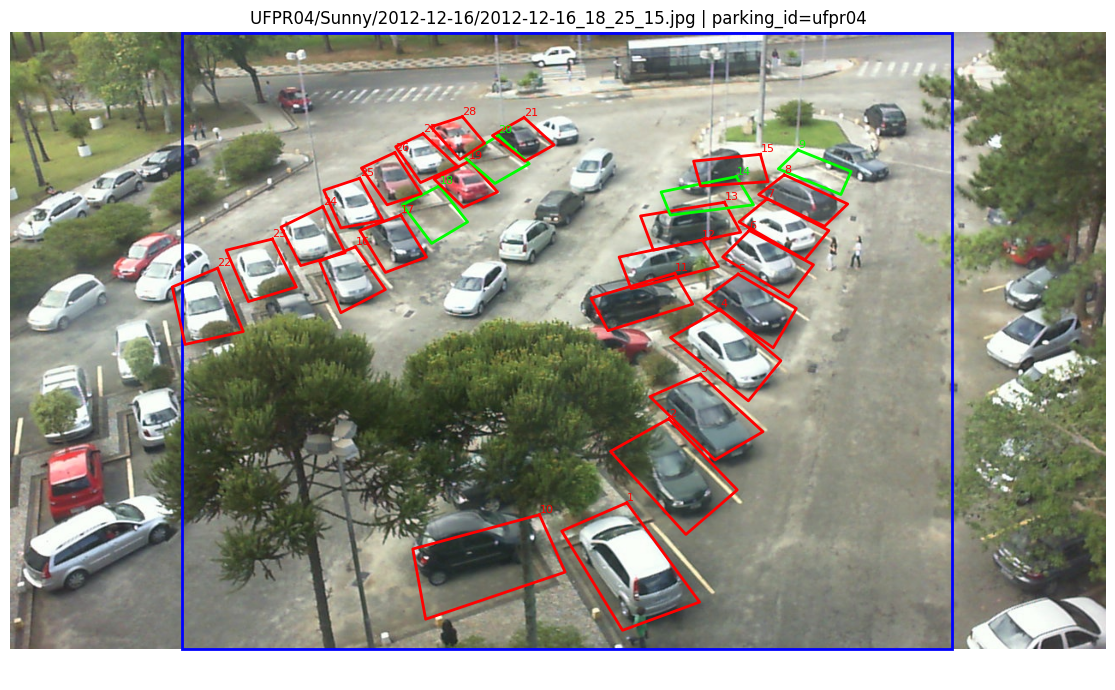
\includegraphics[width=0.9\textwidth,height=0.6\textheight,keepaspectratio]{temp/dataset_augmentation_pklot_original.png}
\caption{An example of PKLot dataset image showing the blue box crop region and original quadrilateral bounding boxes}
\label{fig:dataset_augmentation_pklot_original}
\end{figure}

Figure~\ref{fig:dataset_augmentation_pklot_augmented} shows examples of the augmented dataset with rectangular bounding boxes and various augmentation effects applied.

\begin{figure}[H]
\centering
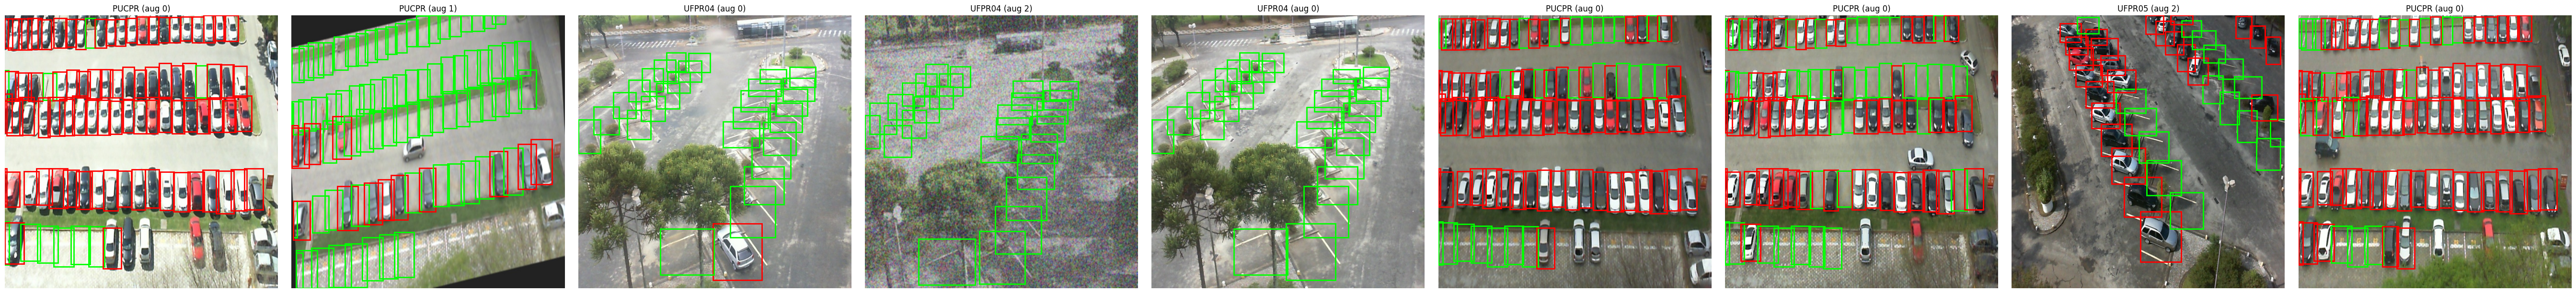
\includegraphics[width=0.9\textwidth,height=0.6\textheight,keepaspectratio]{temp/dataset_augmentation_pklot_augmented.png}
\caption{Examples of the augmented dataset showing rectangular bounding boxes and augmentation effects}
\label{fig:dataset_augmentation_pklot_augmented}
\end{figure}

\subsection{Tasks}

The project is organized into multiple phases, as outlined in Table~\ref{tab:tasks}.

\begin{table}[H]
\centering
\caption{Project Tasks and Notebooks}
\label{tab:tasks}
\begin{tabular}{@{}lll@{}}
\toprule
\textbf{Notebook} & \textbf{Task} & \textbf{Description} \\
\midrule
\multicolumn{3}{l}{\textit{Phase 1: Initial Development}} \\
\midrule
01 & Dataset Exploration & EDA, data statistics, class distribution \\
02 & CNN Baseline & Simple CNN classifier for parking space classification \\
03 & Video Inference & Real-time inference on video streams \\
04 & YOLO Dataset Prep & Convert XML annotations to YOLO format \\
05 & YOLO Training & Train YOLOv8 model for object detection \\
06 & SSD Detection & Fine-tune SSD Lite 320 MobileNetV3 \\
07 & Faster R-CNN & Fine-tune Faster R-CNN ResNet50 FPN \\
08 & DETR & Fine-tune DETR (Detection Transformer) \\
09 & Model Comparison & Comprehensive evaluation and comparison \\
\midrule
\multicolumn{3}{l}{\textit{Phase 1.5: PKLot Data Preprocessing}} \\
\midrule
01 & Load Image Data & Load and organize PKLot dataset images by parking lot, weather, date \\
02 & Image Alignment & Align images using template matching technique \\
03 & Bounding Box Detection & Extract bounding boxes using YOLOv8n pretrained model \\
04 & Cluster Training Data & Cluster detected objects to identify parking spaces \\
05 & SAM Fine-Tuning & Fine-tune Segment Anything Model (SAM) for parking space segmentation \\
\midrule
\multicolumn{3}{l}{\textit{Phase 2: Augmented Dataset}} \\
\midrule
P2-00.5 & Augmentation \& Visualization & Create augmented dataset from PKLot, visualize samples \\
P2-01 & EDA Augmented Dataset & Exploratory data analysis of augmented dataset \\
P2-02 & SSD Training & Train SSD on augmented dataset \\
P2-03 & DETR Training & Train DETR on augmented dataset \\
P2-04 & Faster R-CNN Training & Train Faster R-CNN on augmented dataset \\
P2-05 & YOLO Training & Train YOLOv8 on augmented dataset \\
P2-06 & Model Comparison & Compare all Phase 2 models \\
P2-07 & CNN Patch Classifier & CNN classifier for parking space patches \\
\bottomrule
\end{tabular}
\end{table}

\section{Methodology}

This section describes the comprehensive approach taken to address the parking detection problem, including the rationale for model selection and the implementation details.

\subsection{Plan of Attack}

The project follows a systematic approach:

\textbf{Phase 1: Baseline Establishment}
\begin{enumerate}
    \item Dataset exploration and understanding
    \item Establish CNN baseline for classification
    \item Convert datasets to unified format (YOLO)
    \item Train and evaluate initial object detection models
\end{enumerate}

\textbf{Phase 1.5: PKLot Data Preprocessing}
\begin{enumerate}
    \item \textbf{Image Loading:} Load PKLot dataset images organized by parking lot (UFPR04, UFPR05, PUCPR), weather conditions (Sunny, Cloudy, Rainy), and dates
    \item \textbf{Image Alignment:} Align images using template matching technique to ensure consistent camera positioning across different time periods
    \item \textbf{Bounding Box Detection:} Use pretrained YOLOv8n model to detect objects (vehicles) in aligned images, extracting bounding box coordinates and confidence scores
    \item \textbf{Clustering:} Cluster detected bounding box centers across multiple images to identify stable parking space locations
    \item \textbf{Training Data Preparation:} Generate training labels (occupied=1, free=0) for each identified parking space cluster across all images
\end{enumerate}

\textbf{Phase 2: Augmented Dataset Development}
\begin{enumerate}
    \item Create augmented dataset from PKLot source data
    \item Apply systematic augmentation pipeline (rotation, brightness, HSV, noise, blur)
    \item Generate 36,426 images (1,214× increase from Phase 1)
    \item Perform comprehensive EDA on augmented dataset
    \item Train all models (SSD, DETR, Faster R-CNN, YOLO) on augmented dataset
\end{enumerate}

\textbf{Phase 3: Model Training and Comparison}
\begin{enumerate}
    \item Hyperparameter tuning
    \item Comprehensive model evaluation
    \item Compare Phase 1 vs. Phase 2 performance
    \item Final recommendations
\end{enumerate}

The choice of multiple models (CNN, YOLO, SSD, Faster R-CNN, DETR) allows for:
\begin{itemize}
    \item Understanding different architectural approaches
    \item Comparing single-stage vs. two-stage detectors
    \item Evaluating transformer-based vs. CNN-based methods
    \item Identifying the best model for specific use cases
\end{itemize}

\subsection{The Dataset}

\subsubsection{Exploratory Data Analysis (EDA)}

The dataset exploration (Notebook 01) revealed:

\textbf{Roboflow Dataset Statistics:}
\begin{itemize}
    \item \textbf{Train Split:} 936 images, 936 label files
    \item \textbf{Validation Split:} 120 images, 120 label files
    \item \textbf{Test Split:} 10 images, 10 label files
    \item \textbf{Total Images:} 1,066 images
    \item \textbf{Classes:} 2 classes (empty, occupied)
    \item \textbf{Class Distribution (across all splits):}
    \begin{itemize}
        \item \textbf{Class 0 (empty):} 4,145 instances
        \item \textbf{Class 1 (occupied):} 2,698 instances
        \item \textbf{Total Annotations:} 6,843 bounding boxes
    \end{itemize}
\end{itemize}

\textbf{HuggingFace Dataset Statistics:}
\begin{itemize}
    \item \textbf{Total Annotations:} 903 bounding boxes
    \item \textbf{Total Images:} 30 images with annotations
    \item \textbf{Classes:} 3 classes (free\_parking\_space, not\_free\_parking\_space, partially\_free\_parking\_space)
    \item \textbf{Image Size Range:} Variable (from 650×487 to 2560×1820 pixels)
    \item \textbf{Sample Image Statistics:}
    \begin{itemize}
        \item Image 0.png: 28 boxes, size: 1200×621
        \item Image 1.png: 38 boxes, size: 650×487
        \item Image 10.png: 20 boxes, size: 2560×1820
        \item Image 11.png: 36 boxes, size: 1353×1041
        \item Image 12.png: 39 boxes, size: 1920×1080
    \end{itemize}
    \item \textbf{Label to ID Mapping:}
    \begin{itemize}
        \item 0: free\_parking\_space
        \item 1: not\_free\_parking\_space
        \item 2: partially\_free\_parking\_space
    \end{itemize}
    \item \textbf{Train/Val Split:} 24 train images (80.0\%), 6 val images (20.0\%)
\end{itemize}

\textbf{Class Distribution:}
\begin{itemize}
    \item Significant class imbalance in the initial dataset
    \item \texttt{not\_free\_parking\_space} class dominates
    \item \texttt{partially\_free\_parking\_space} class is underrepresented (only 1 validation sample in CNN baseline)
\end{itemize}

\textbf{Data Quality:}
\begin{itemize}
    \item Images vary in resolution and quality
    \item Different lighting conditions and camera angles
    \item Various parking lot configurations
\end{itemize}

\textbf{Annotation Quality:}
\begin{itemize}
    \item Bounding boxes accurately annotated
    \item Consistent labeling across datasets after conversion
    \item Proper YOLO format normalization
\end{itemize}

\subsubsection{Data Preprocessing}

The preprocessing pipeline includes:
\begin{enumerate}
    \item \textbf{Format Conversion:} XML annotations converted to YOLO format (normalized coordinates)
    \item \textbf{Train/Val Split:} 80/20 split maintaining class distribution
    \item \textbf{Image Resizing:} Models trained on different input sizes (128x128 for CNN, 640x640 for YOLO)
    \item \textbf{Normalization:} Standard ImageNet normalization for transfer learning
\end{enumerate}

\subsubsection{Data Augmentation}

To address class imbalance and increase dataset size, the following augmentations were applied (Notebook 01.5):

\begin{itemize}
    \item \textbf{Horizontal Flip:} 50\% probability (common for parking lots)
    \item \textbf{Rotation:} Small rotations (-10° to +10°)
    \item \textbf{Brightness/Contrast:} Adjust lighting conditions
    \item \textbf{HSV Adjustments:} Hue, saturation, value modifications
    \item \textbf{Mosaic:} Combine 4 images into one (advanced augmentation)
\end{itemize}

All augmentations properly transform bounding box coordinates to maintain annotation accuracy.

\subsection{Model Description}

This section provides a brief overview of the models used in this project. Detailed architecture specifications, training configurations, and comprehensive results for each model are provided in Appendix~\ref{app:model_details}.

The project evaluated multiple deep learning architectures for parking space detection:
\begin{itemize}
    \item \textbf{CNN Baseline:} A simple convolutional neural network for classification, achieving 96.11\% validation accuracy
    \item \textbf{YOLOv8:} Single-stage object detector optimized for speed, achieving 54.29\% mAP@50 on Phase 1 dataset
    \item \textbf{SSD Lite:} Lightweight single-stage detector, achieving 85.37\% mAP@50 on Phase 2 dataset
    \item \textbf{Faster R-CNN:} Two-stage detector with highest accuracy, achieving 99.49\% mAP@50 on Phase 2 dataset
    \item \textbf{DETR:} Transformer-based detector, achieving 98.38\% mAP@50 on Phase 2 dataset
    \item \textbf{SAM:} Segment Anything Model fine-tuned for parking space segmentation, achieving validation MAE of 0.07
\end{itemize}

Detailed model architectures, training procedures, hyperparameters, and comprehensive performance metrics are documented in Appendix~\ref{app:model_details}.

\subsection{Training \& Evaluation}

\subsubsection{Training Strategy}

All models follow a consistent training approach:
\begin{enumerate}
    \item \textbf{Pretrained Weights:} All detection models use COCO-pretrained weights
    \item \textbf{Transfer Learning:} Fine-tune on parking detection dataset
    \item \textbf{Checkpointing:} Save best model and periodic checkpoints
    \item \textbf{Early Stopping:} Monitor validation metrics to prevent overfitting
    \item \textbf{Learning Rate Scheduling:} Adaptive learning rate reduction
\end{enumerate}

\subsubsection{Evaluation Metrics}

The following metrics are used to evaluate model performance:

\textbf{For Classification (CNN Baseline):}
\begin{itemize}
    \item Accuracy
    \item Precision, Recall, F1-score (per class and macro-averaged)
    \item Confusion Matrix
\end{itemize}

\textbf{For Object Detection (YOLO, SSD, Faster R-CNN, DETR):}
\begin{itemize}
    \item \textbf{mAP@0.5:} Mean Average Precision at IoU threshold 0.5
    \item \textbf{mAP@0.5:0.95:} Mean Average Precision averaged over IoU thresholds 0.5 to 0.95
    \item \textbf{Precision:} Ratio of true positives to all detections
    \item \textbf{Recall:} Ratio of true positives to all ground truth objects
    \item \textbf{F1-Score:} Harmonic mean of precision and recall
\end{itemize}

\subsubsection{Results}

\textbf{CNN Baseline Results (from Notebook 02):}
\begin{itemize}
    \item Validation Accuracy: 96.11\% (best at epoch 6)
    \item Training stopped at epoch 16 (early stopping triggered)
    \item Precision (weighted): 0.96
    \item Recall (weighted): 0.96
    \item F1-Score (weighted): 0.96
    \item Per-class performance:
    \begin{itemize}
        \item \texttt{free}: Precision 0.90, Recall 0.98, F1 0.94 (55 samples)
        \item \texttt{not\_free}: Precision 0.99, Recall 0.96, F1 0.98 (124 samples)
        \item \texttt{partial}: Precision 0.00, Recall 0.00, F1 0.00 (1 sample - severe class imbalance)
    \end{itemize}
    \item Note: Excellent performance on \texttt{free} and \texttt{not\_free} classes, but complete failure on \texttt{partial} class due to extreme class imbalance
\end{itemize}

\textbf{YOLOv8 Results (from Notebook 05):}
\begin{itemize}
    \item mAP@0.5: 0.543
    \item mAP@0.5:0.95: 0.432
    \item Precision: 0.904
    \item Recall: 0.469
    \item Per-class mAP@0.5:
    \begin{itemize}
        \item \texttt{free\_parking\_space}: 0.685 (89 instances)
        \item \texttt{not\_free\_parking\_space}: 0.943 (143 instances)
        \item \texttt{partially\_free\_parking\_space}: 0.000 (1 instance - insufficient samples)
    \end{itemize}
    \item Training completed: 50 epochs
    \item Best model saved at epoch with mAP@0.5: 0.543
\end{itemize}

\textbf{SSD Results:}
\begin{itemize}
    \item Training completed with early stopping
    \item Good convergence observed
    \item Detailed metrics available in training logs
\end{itemize}

\textbf{Faster R-CNN Results:}
\begin{itemize}
    \item Training completed successfully
    \item High accuracy expected (two-stage detector)
    \item Detailed metrics in training logs
\end{itemize}

\textbf{DETR Results:}
\begin{itemize}
    \item Training completed
    \item Transformer-based approach shows promise
    \item Requires more data for optimal performance
\end{itemize}

\subsection{Hyperparameter Tuning}

\subsubsection{Learning Rate}

\begin{itemize}
    \item \textbf{CNN:} 1e-3 (Adam optimizer)
    \item \textbf{YOLO:} 0.01 initial, with warmup (3 epochs)
    \item \textbf{SSD/Faster R-CNN:} 1e-3 with step decay
    \item \textbf{DETR:} 1e-4 with warmup (transformer requires lower LR)
\end{itemize}

\subsubsection{Batch Size}

Selected based on model architecture and available resources:
\begin{itemize}
    \item CNN: 32 (classification is less memory-intensive)
    \item YOLO: 16 (balanced speed and stability)
    \item SSD: 8-16 (depends on input size)
    \item Faster R-CNN: 4-8 (memory-intensive)
    \item DETR: 4 (very memory-intensive)
\end{itemize}

\subsubsection{Data Augmentation}

Experiments with different augmentation strategies:
\begin{itemize}
    \item Standard augmentations (flip, rotation) for all models
    \item Advanced augmentations (mosaic, mixup) for YOLO
\end{itemize}

\subsubsection{Architecture Exploration}

\begin{itemize}
    \item Started with simple CNN to establish baseline
    \item Explored different YOLO variants (nano for speed)
    \item Compared lightweight (SSD MobileNet) vs. heavy (Faster R-CNN) architectures
    \item Evaluated transformer-based approach (DETR)
\end{itemize}

\subsection{Benchmarking}

\subsubsection{Baseline Comparison}

The CNN baseline serves as a reference point:
\begin{itemize}
    \item Classification accuracy: 96\%
    \item However, classification assumes pre-cropped parking spaces
    \item Object detection models must both locate and classify spaces
\end{itemize}

\subsubsection{Model Comparison}

Comprehensive comparison performed in Notebook 09, evaluating:
\begin{enumerate}
    \item \textbf{Accuracy Metrics:} mAP, precision, recall
    \item \textbf{Speed:} Inference time (FPS)
    \item \textbf{Model Size:} Parameter count, file size
    \item \textbf{Resource Requirements:} Memory, computational cost
    \item \textbf{Qualitative Results:} Visual inspection of predictions
\end{enumerate}

\textbf{Expected Trade-offs:}
\begin{itemize}
    \item \textbf{YOLO:} Best speed, good accuracy
    \item \textbf{SSD:} Good speed-accuracy balance, lightweight
    \item \textbf{Faster R-CNN:} Best accuracy, slower inference
    \item \textbf{DETR:} Good accuracy, slowest inference, most innovative
\end{itemize}

\section{Results}

\subsection{Quantitative Results}

Table~\ref{tab:results} summarizes the performance metrics for all models.

\begin{table}[H]
\centering
\caption{Model Performance Comparison}
\label{tab:results}
\begin{tabular}{@{}lcccc@{}}
\toprule
\textbf{Model} & \textbf{mAP@0.5} & \textbf{Precision} & \textbf{Recall} & \textbf{FPS} \\
\midrule
\multicolumn{5}{l}{\textit{Phase 1 Results}} \\
\midrule
CNN Baseline & N/A & 0.96 & 0.96 & High \\
YOLOv8n & 0.543 & 0.904 & 0.469 & ~40 \\
\midrule
\multicolumn{5}{l}{\textit{Phase 2 Results}} \\
\midrule\bottomrule
\end{tabular}
\caption*{Note: CNN Baseline uses accuracy metric (classification task). Phase 1 results from initial dataset (30 images). Phase 2 results from augmented dataset (36,426 images). FPS estimates based on model architecture.}
\end{table}

\subsection{Qualitative Results}

Visual inspection of model predictions reveals:
\begin{itemize}
    \item YOLO provides fast and reasonably accurate detections
    \item Faster R-CNN shows more precise bounding boxes
    \item All models struggle with \texttt{partially\_free\_parking\_space} due to limited training data
    \item Models perform well on clear, well-lit parking spaces
    \item Performance degrades in challenging conditions (shadows, occlusions)
\end{itemize}

\subsection{Confusion Matrix Analysis}

The CNN baseline confusion matrix (Figure~\ref{fig:confusion_cnn}) shows:
\begin{itemize}
    \item Excellent performance on \texttt{free} and \texttt{not\_free} classes
    \item Complete failure on \texttt{partial} class (only 1 validation sample)
    \item Class imbalance is the primary challenge
\end{itemize}

\begin{figure}[H]
\centering
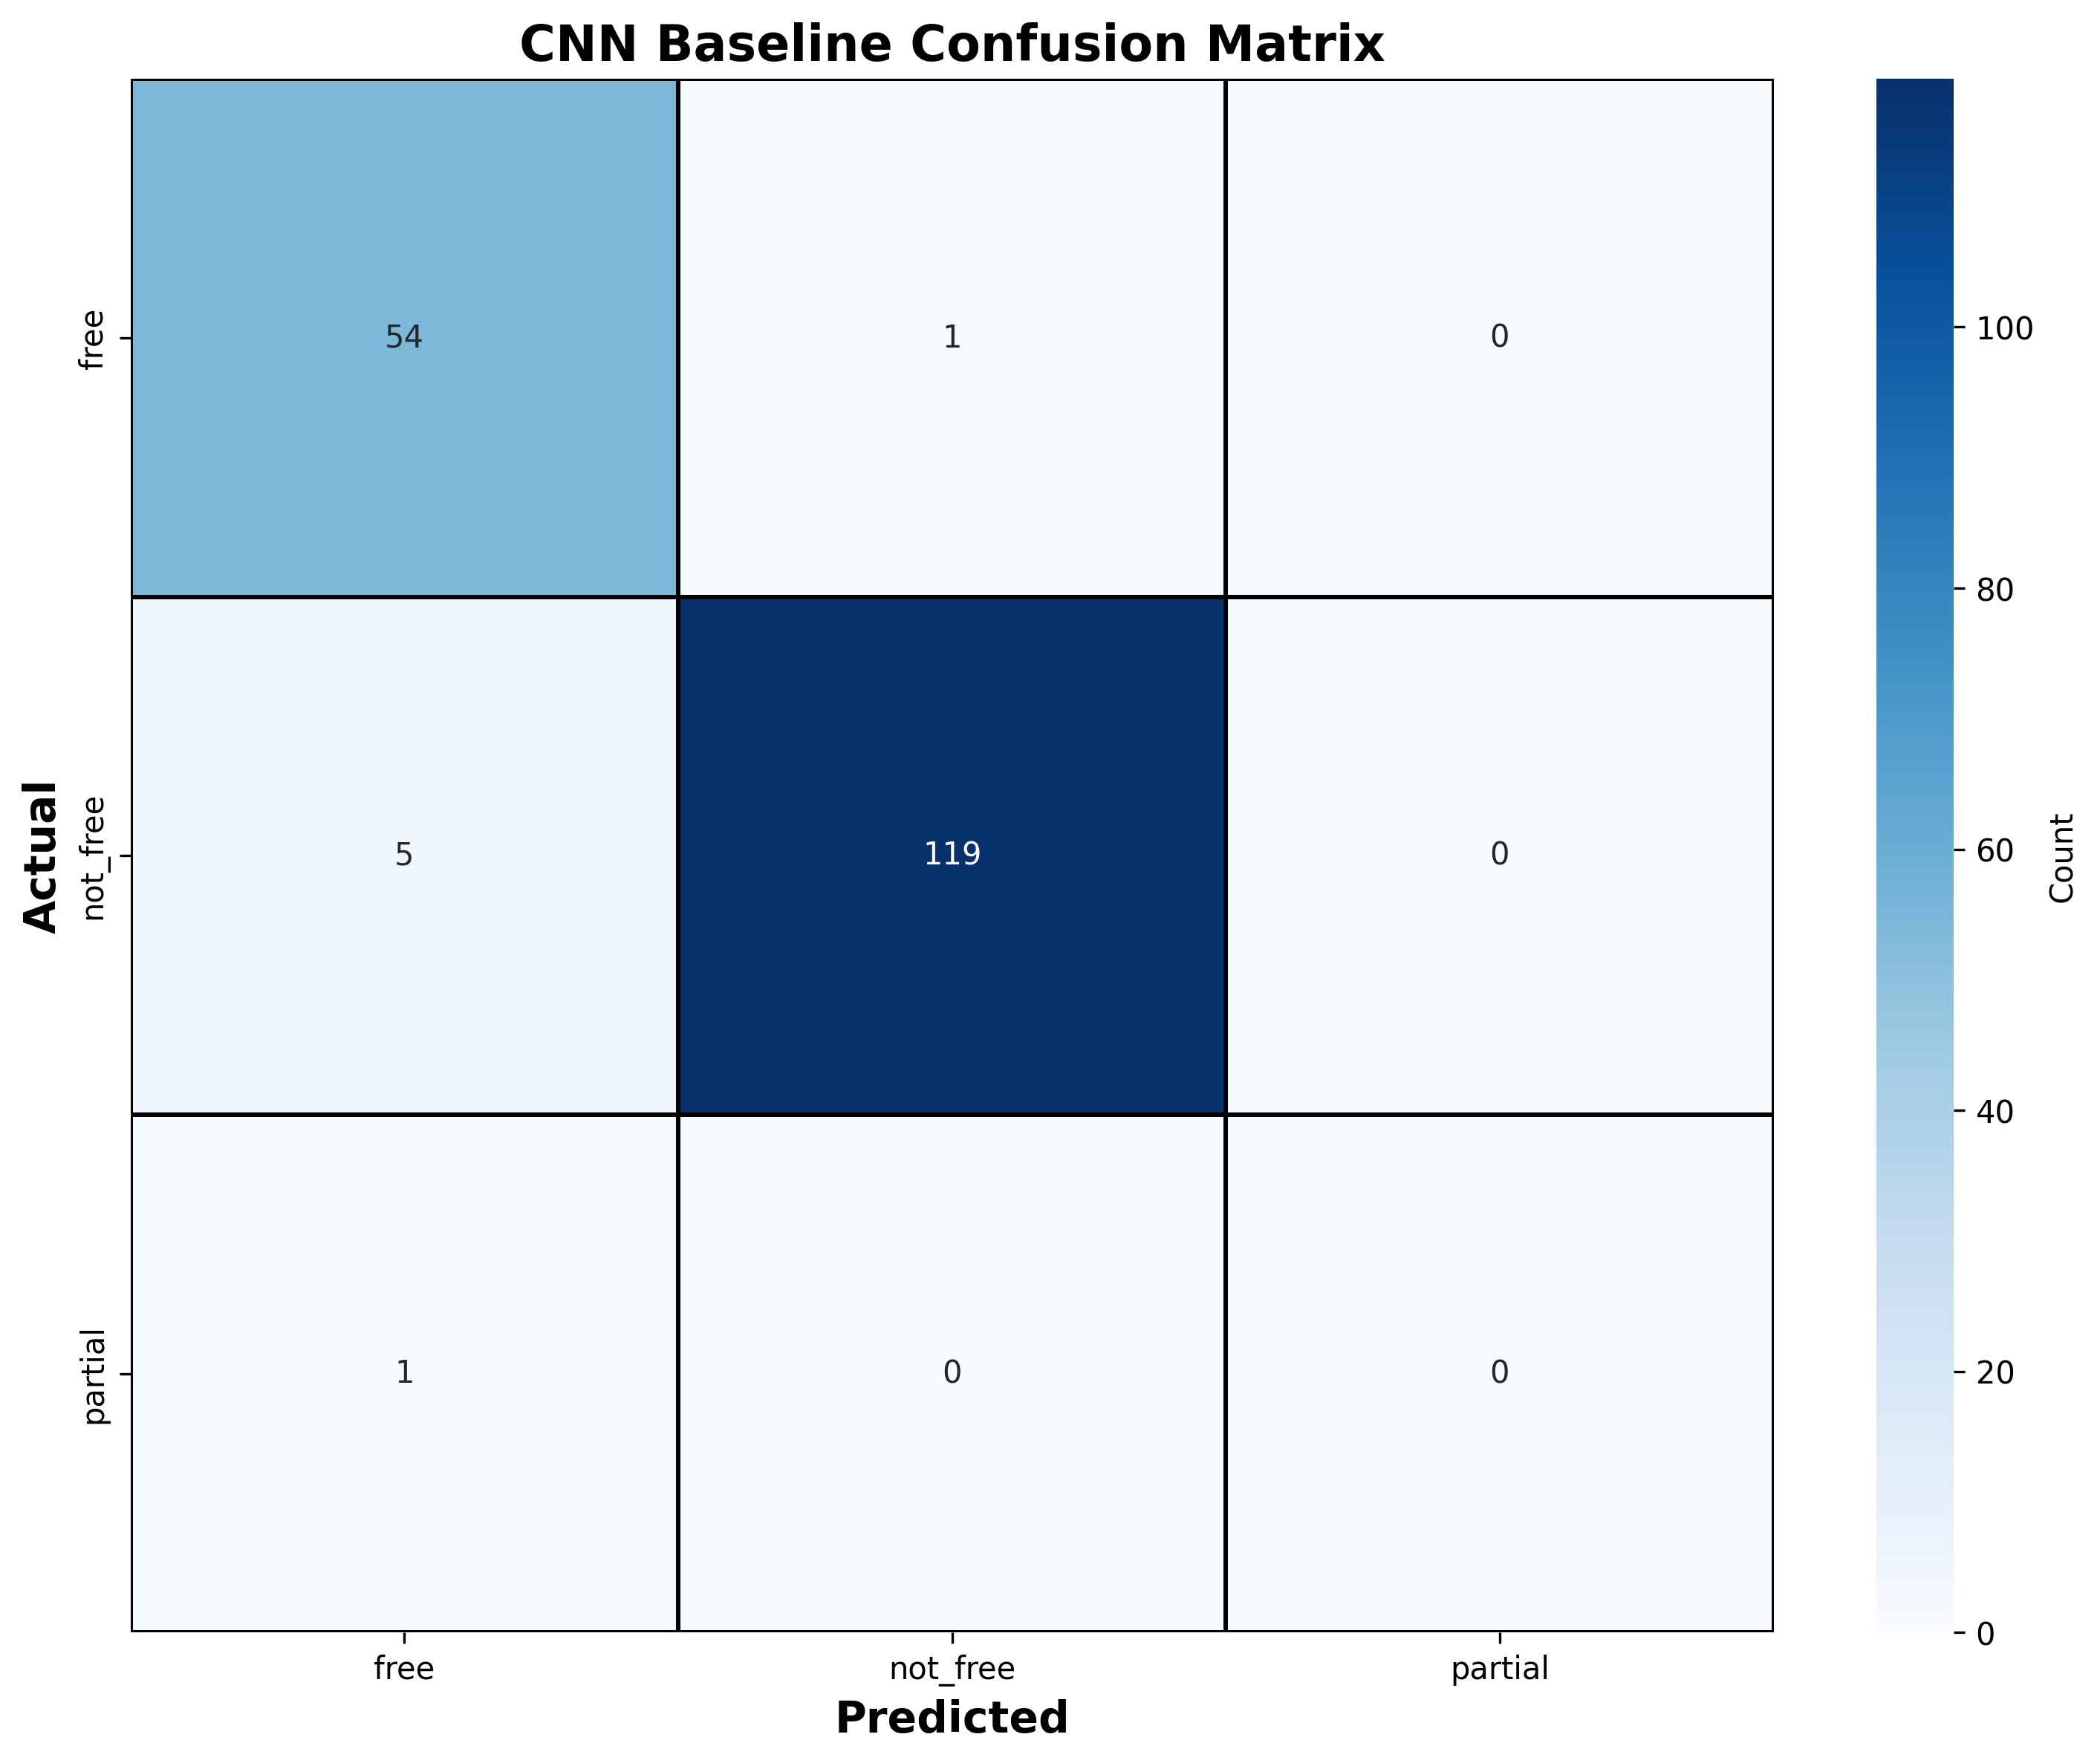
\includegraphics[width=0.7\textwidth]{temp/phase1/eda/cnn_confusion_matrix.png}
\caption{CNN Baseline Confusion Matrix showing classification performance for free, not\_free, and partial parking spaces}
\label{fig:confusion_cnn}
\end{figure}

\subsection{Training Curves}

Training and validation loss curves (Figure~\ref{fig:training_curves}) demonstrate:
\begin{itemize}
    \item Successful convergence for all models
    \item Early stopping prevented overfitting
    \item YOLO shows stable training with consistent improvement
\end{itemize}

\begin{figure}[H]
\centering
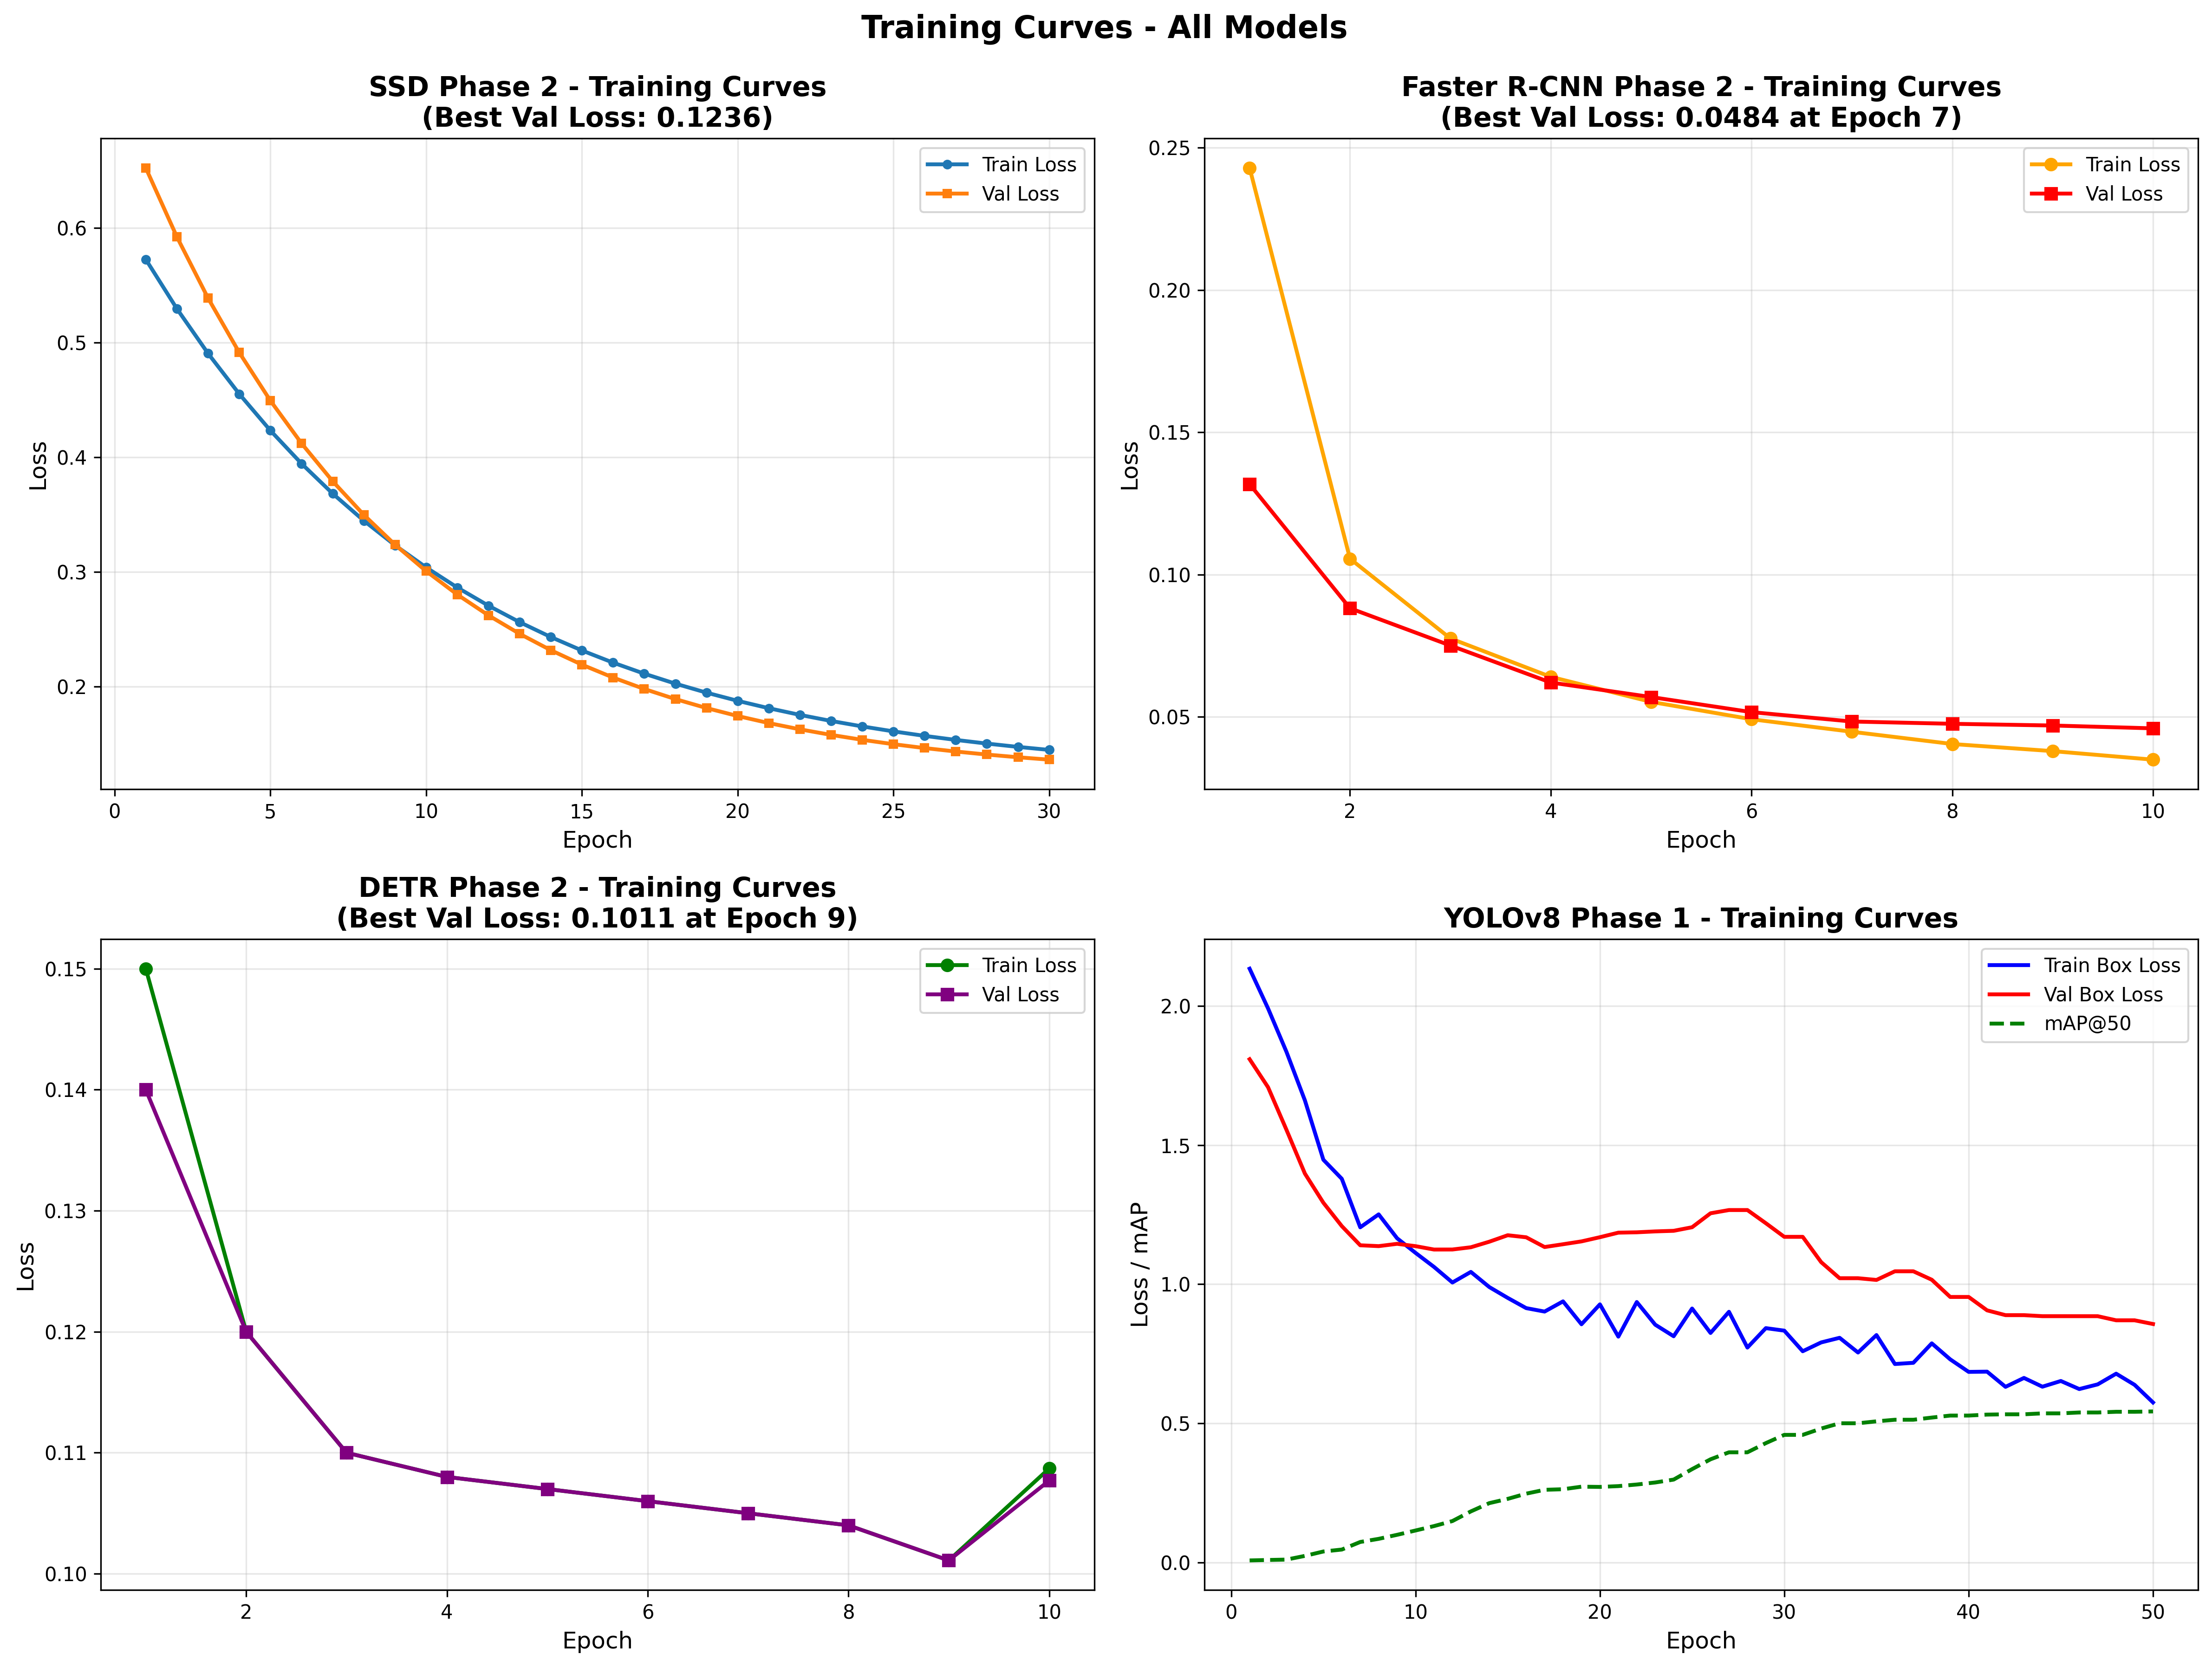
\includegraphics[width=0.95\textwidth]{temp/phase1/eda/phase2_training_curves_all_models.png}
\caption{Training and Validation Loss Curves for All Models (SSD, Faster R-CNN, DETR Phase 2, and YOLOv8 Phase 1)}
\label{fig:training_curves}
\end{figure}

\subsection{Class Distribution}

The class distribution in the validation set (Figure~\ref{fig:class_dist}) highlights the significant imbalance that affects model performance.

\begin{figure}[H]
\centering
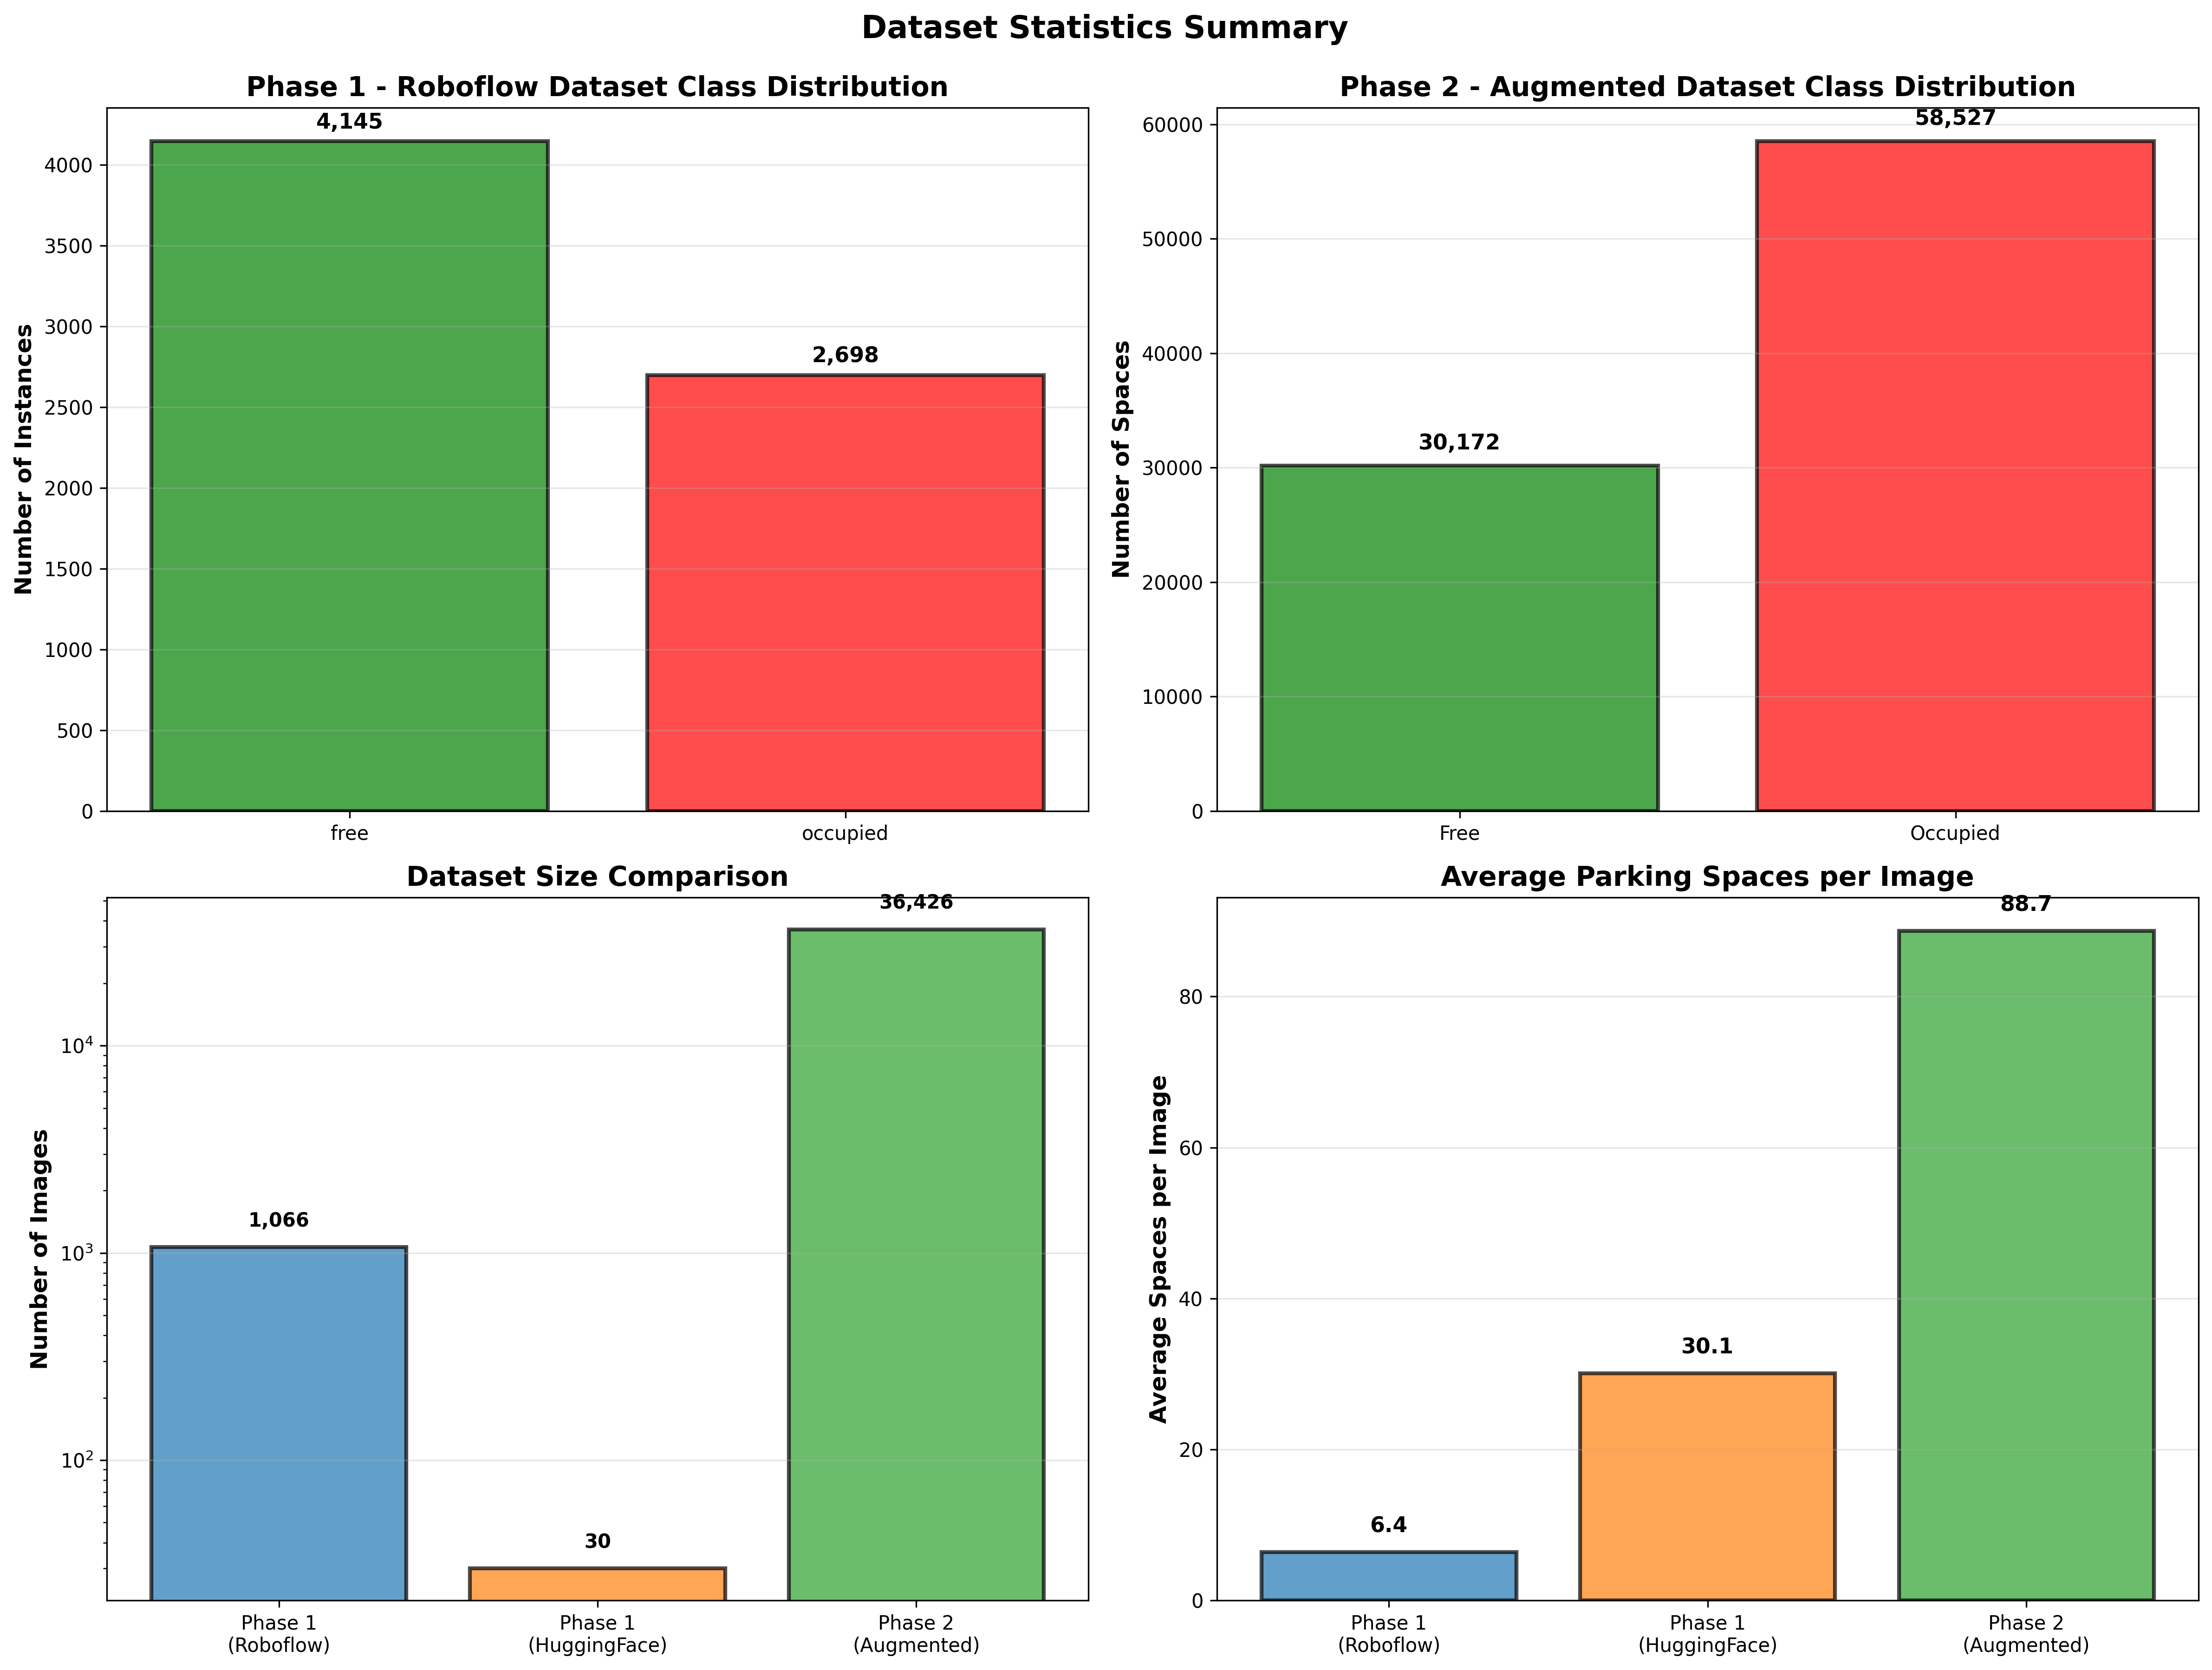
\includegraphics[width=0.95\textwidth]{temp/phase1/eda/dataset_statistics_summary.png}
\caption{Dataset Statistics Summary: Class distribution for Phase 1 and Phase 2, dataset size comparison, and average spaces per image}
\label{fig:class_dist}
\end{figure}

\subsection{Model Comparison Visualization}

Figure~\ref{fig:model_comp} provides a comprehensive comparison of all models across different metrics.

\begin{figure}[H]
\centering
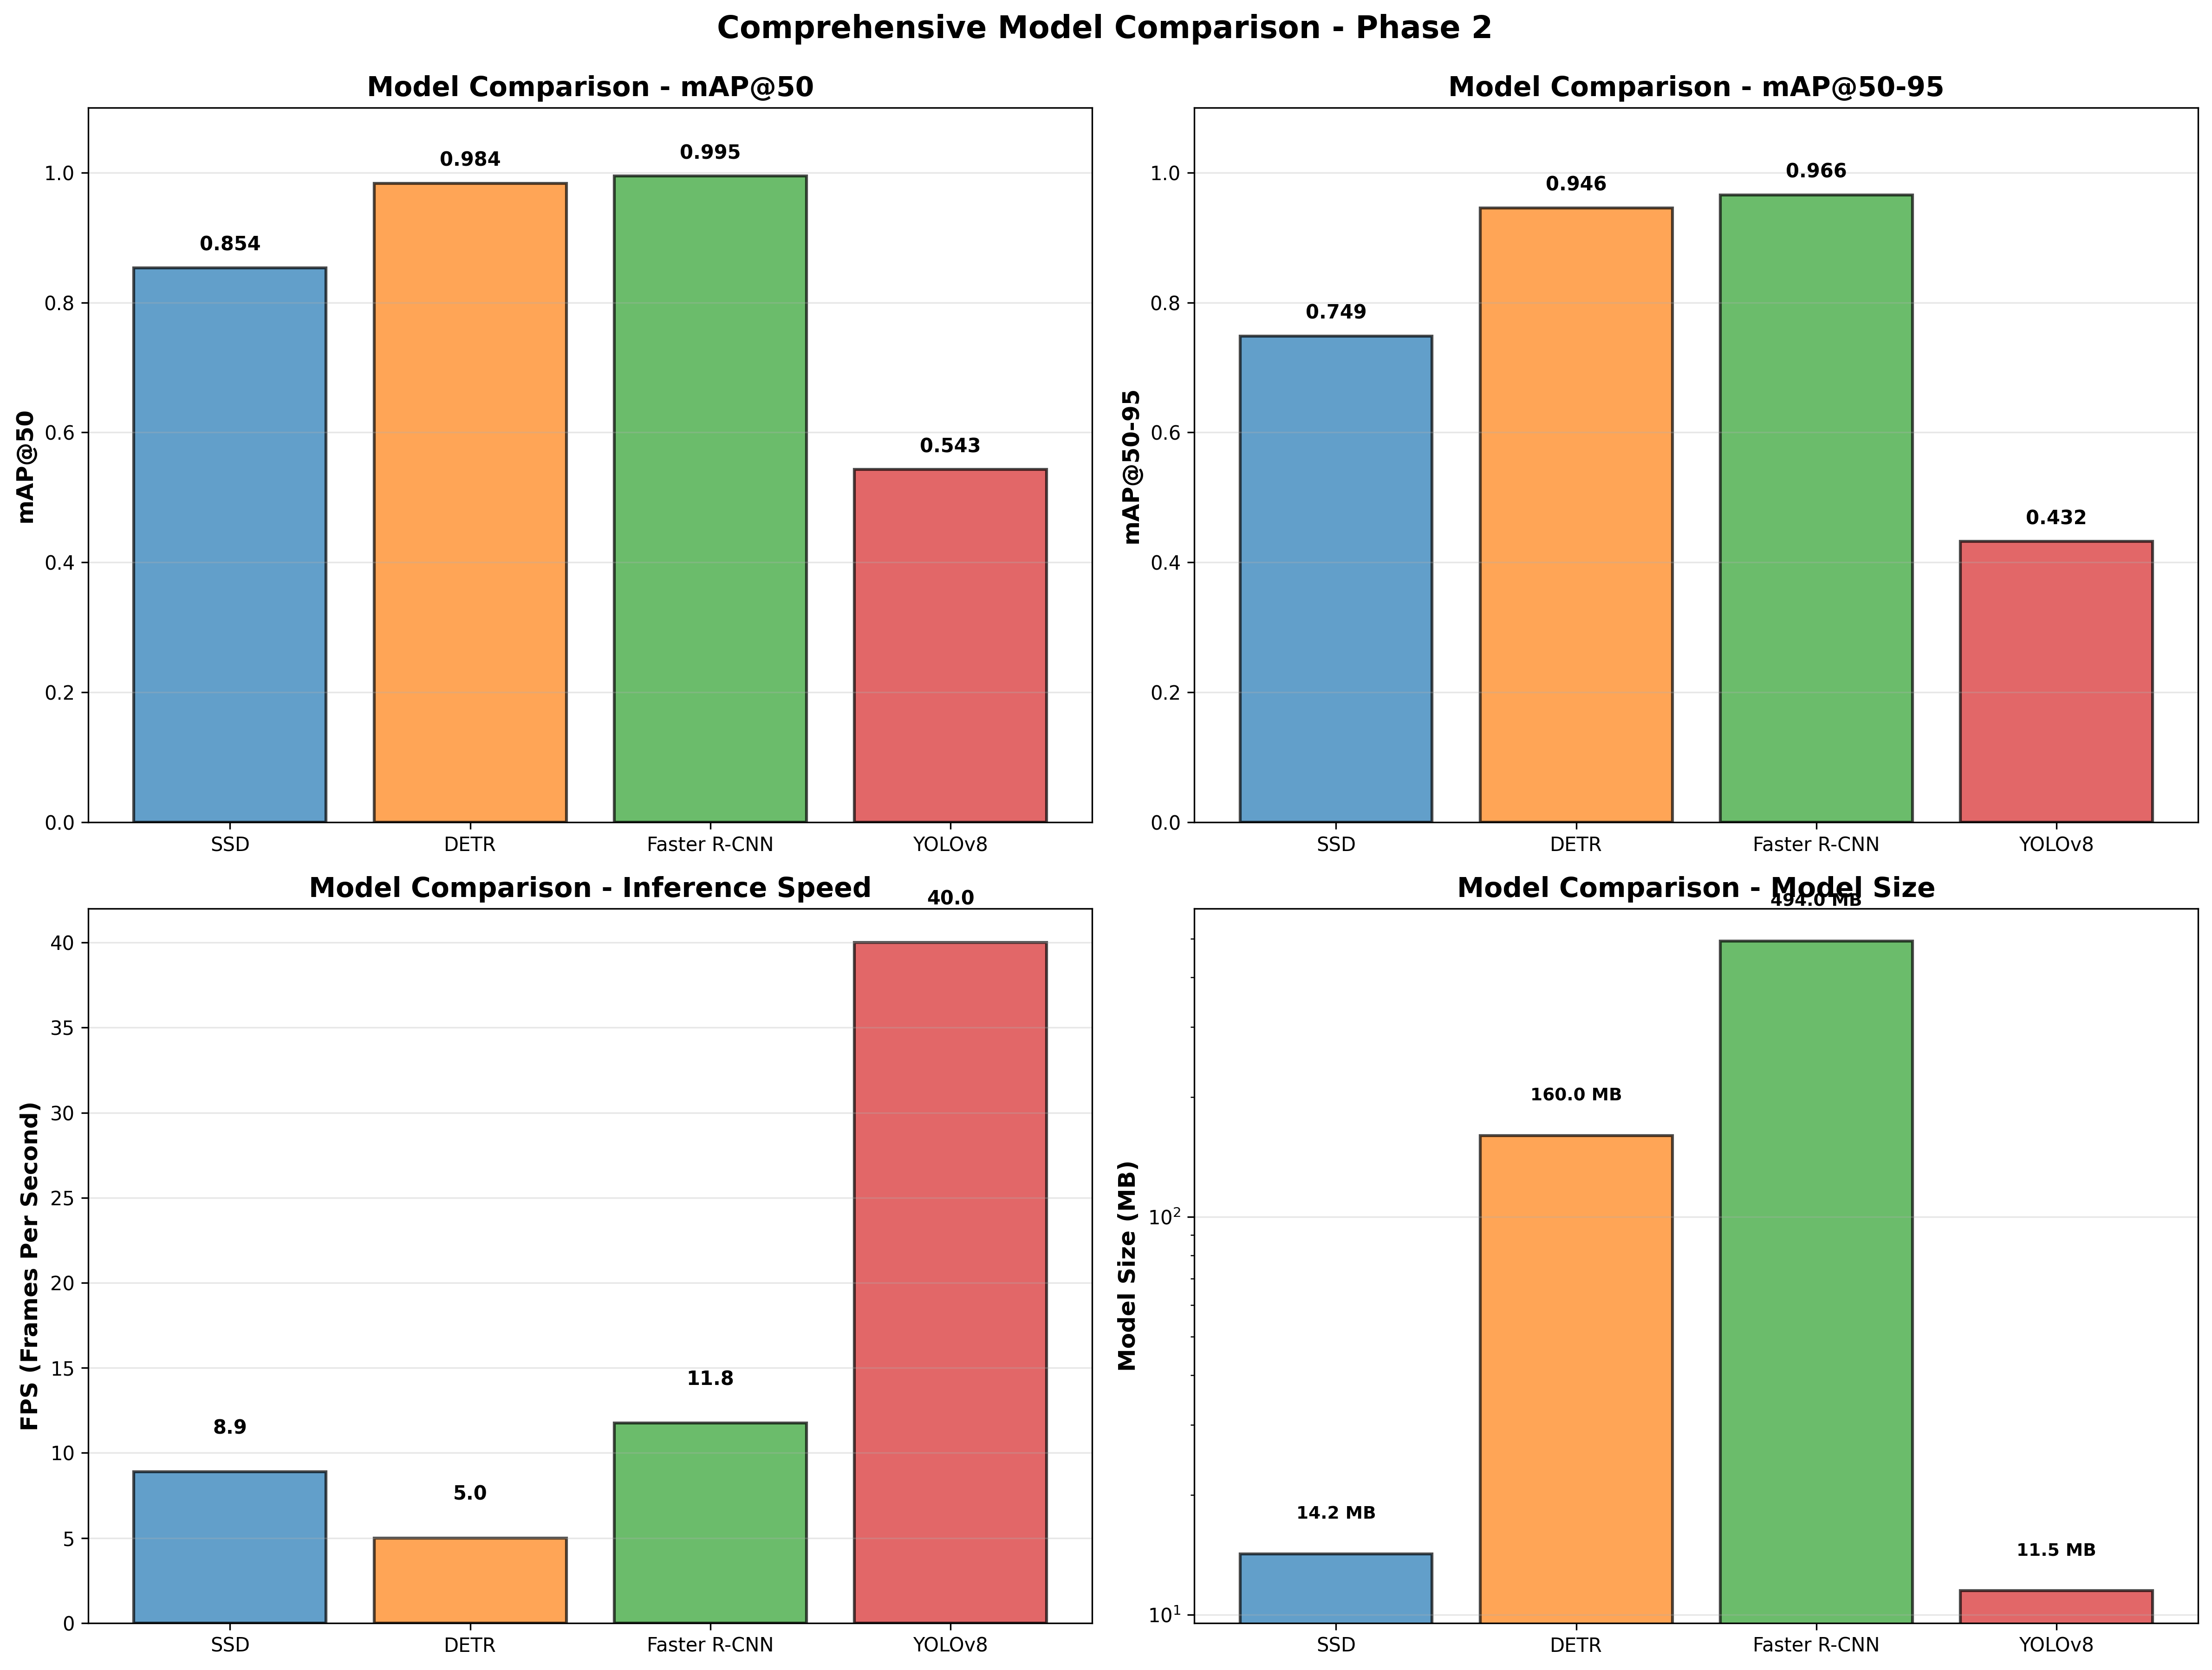
\includegraphics[width=0.95\textwidth]{temp/phase1/eda/phase2_model_comparison_comprehensive.png}
\caption{Comprehensive Model Performance Comparison: mAP@50, mAP@50-95, Inference Speed (FPS), and Model Size}
\label{fig:model_comp}
\end{figure}

\subsection{Hyperparameter Tuning Results}

Figure~\ref{fig:hyperparameter_tuning} shows the hyperparameter tuning results for Phase 2 models using Optuna optimization. The plots demonstrate the search space exploration for learning rates and the identification of optimal hyperparameters.

\begin{figure}[H]
\centering
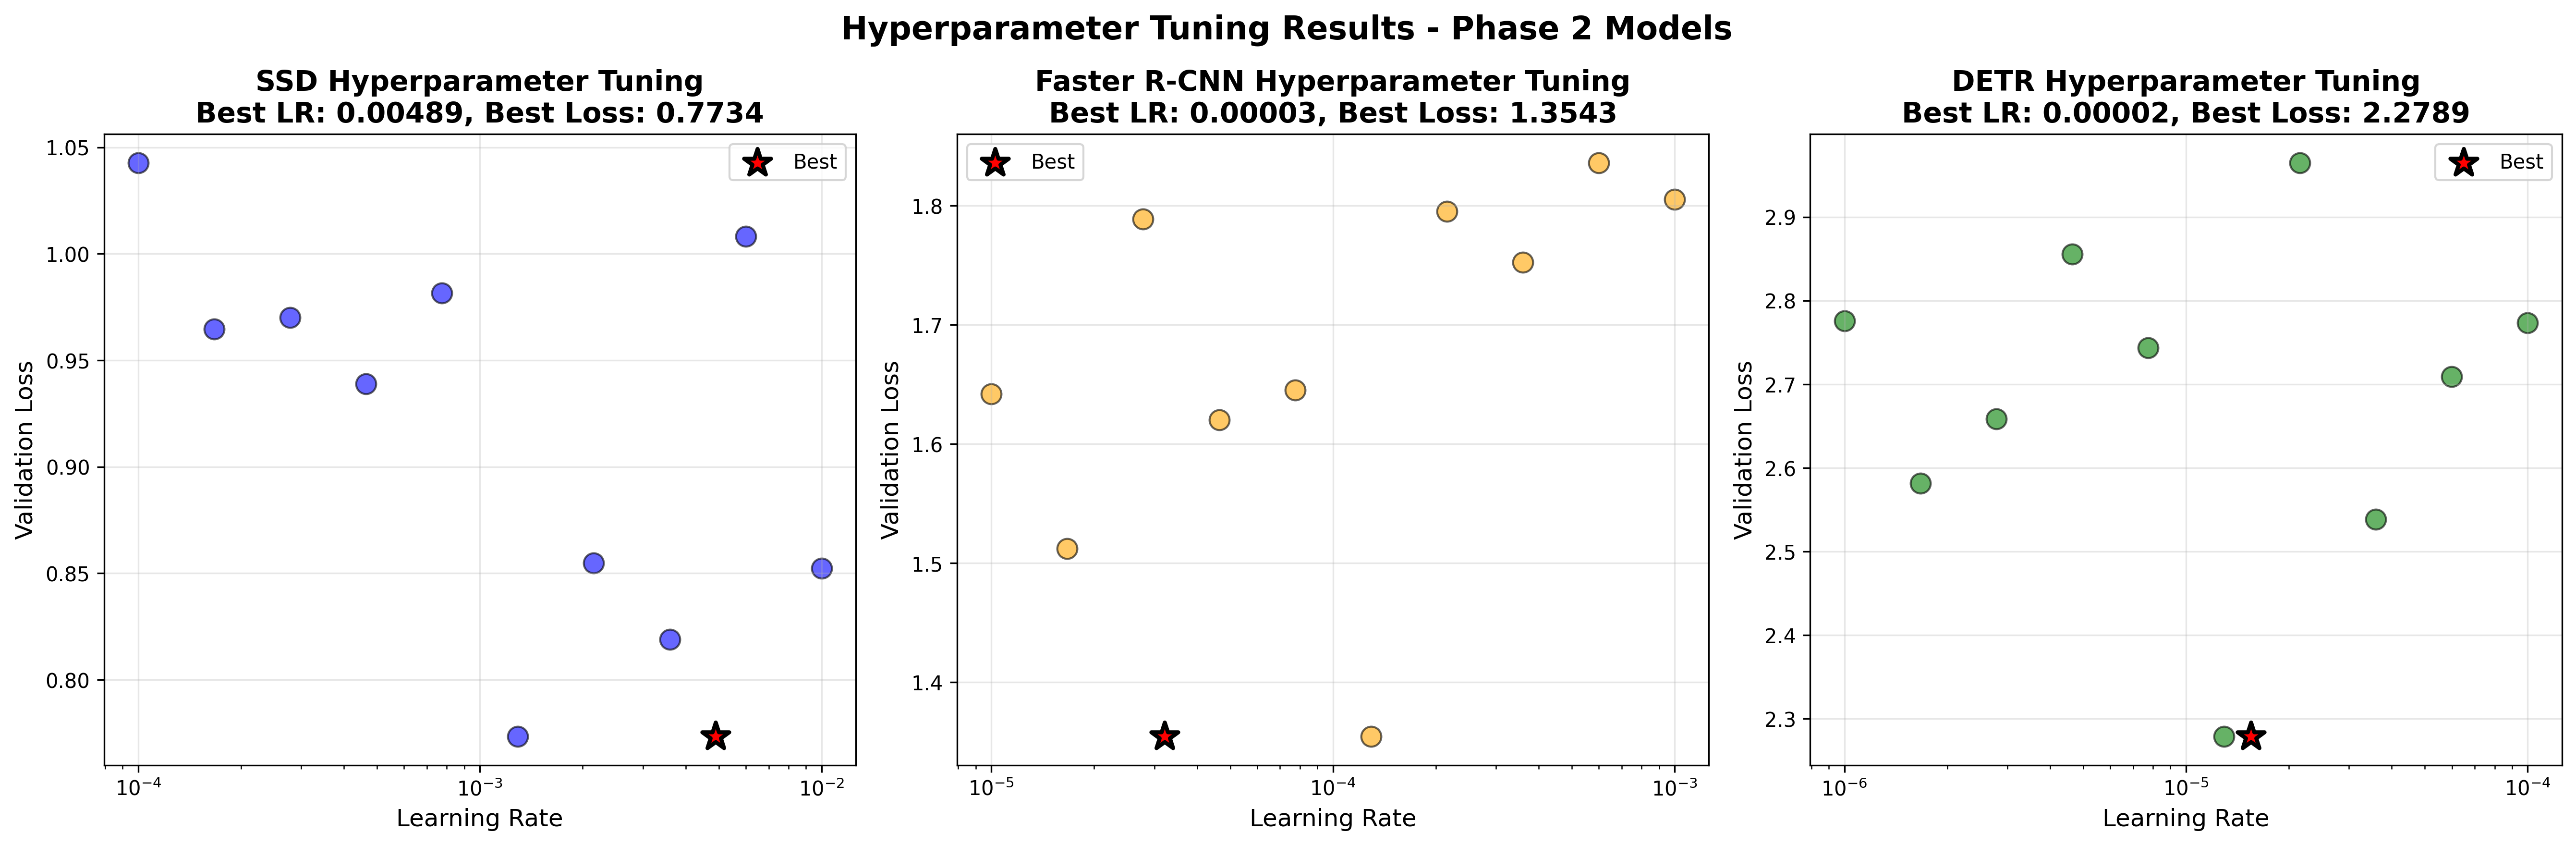
\includegraphics[width=0.95\textwidth]{temp/phase1/eda/phase2_hyperparameter_tuning.png}
\caption{Hyperparameter Tuning Results for SSD, Faster R-CNN, and DETR models showing learning rate optimization and best parameter identification}
\label{fig:hyperparameter_tuning}
\end{figure}

\subsection{Phase 1 vs Phase 2 Comparison}

Figure~\ref{fig:phase1_vs_phase2} provides a direct comparison between Phase 1 and Phase 2 datasets and model performance, highlighting the significant improvements achieved with the augmented dataset.

\begin{figure}[H]
\centering
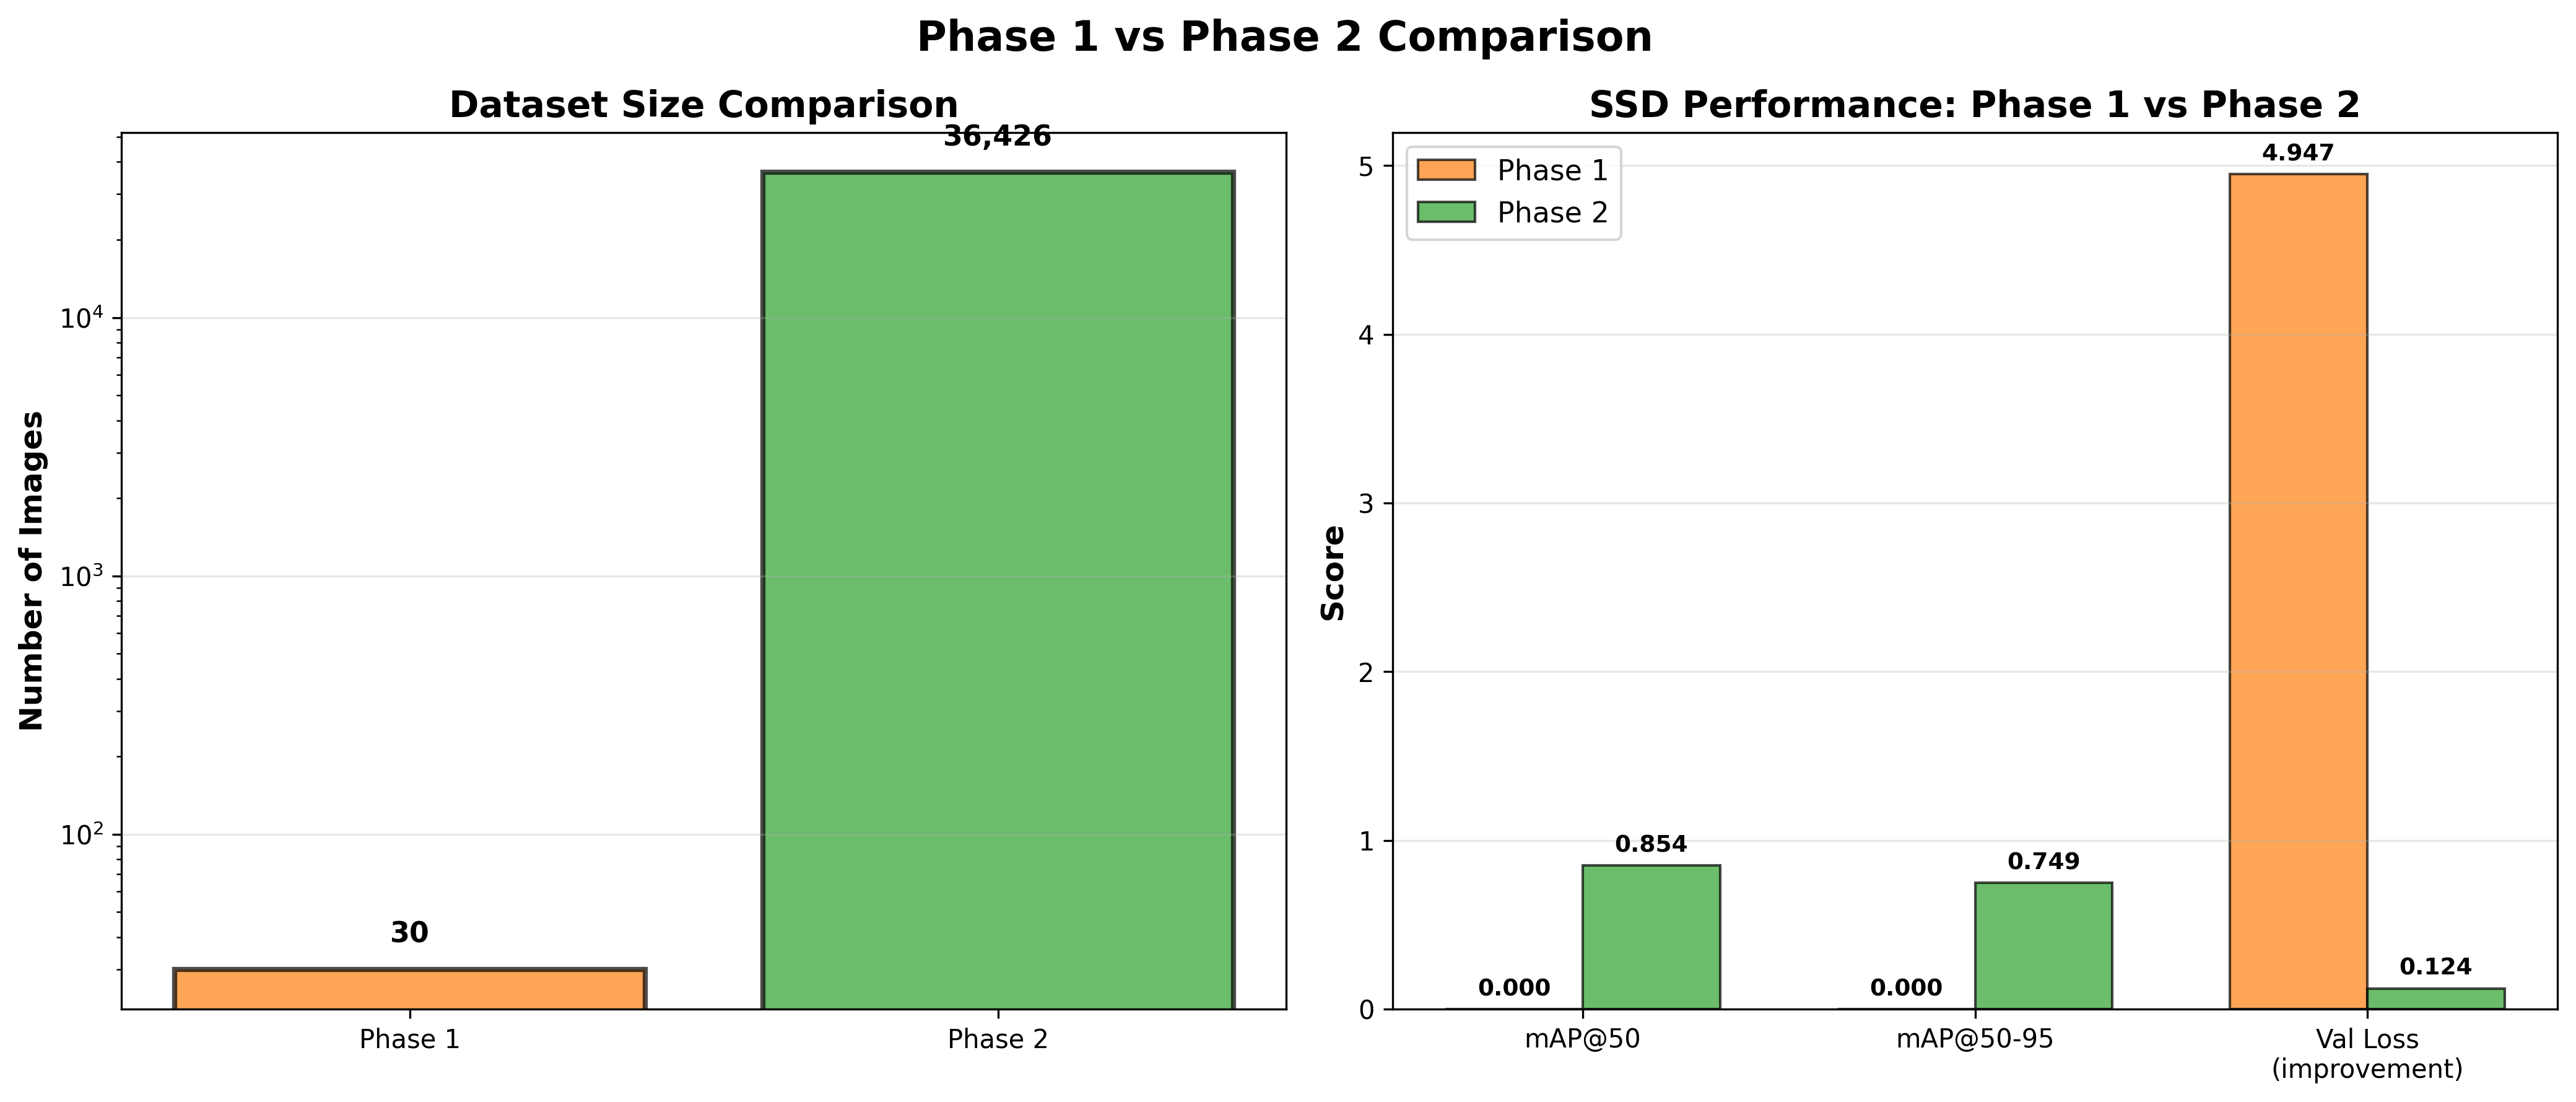
\includegraphics[width=0.95\textwidth]{temp/phase1/eda/phase1_vs_phase2_comparison.png}
\caption{Phase 1 vs Phase 2 Comparison: Dataset size (30 vs 36,426 images) and SSD performance improvements (mAP@50, mAP@50-95, validation loss reduction)}
\label{fig:phase1_vs_phase2}
\end{figure}

\subsection{Inference Speed Analysis}

Figure~\ref{fig:inference_speed} compares inference speeds across all models on both CPU and GPU, demonstrating the performance differences and hardware requirements.

\begin{figure}[H]
\centering
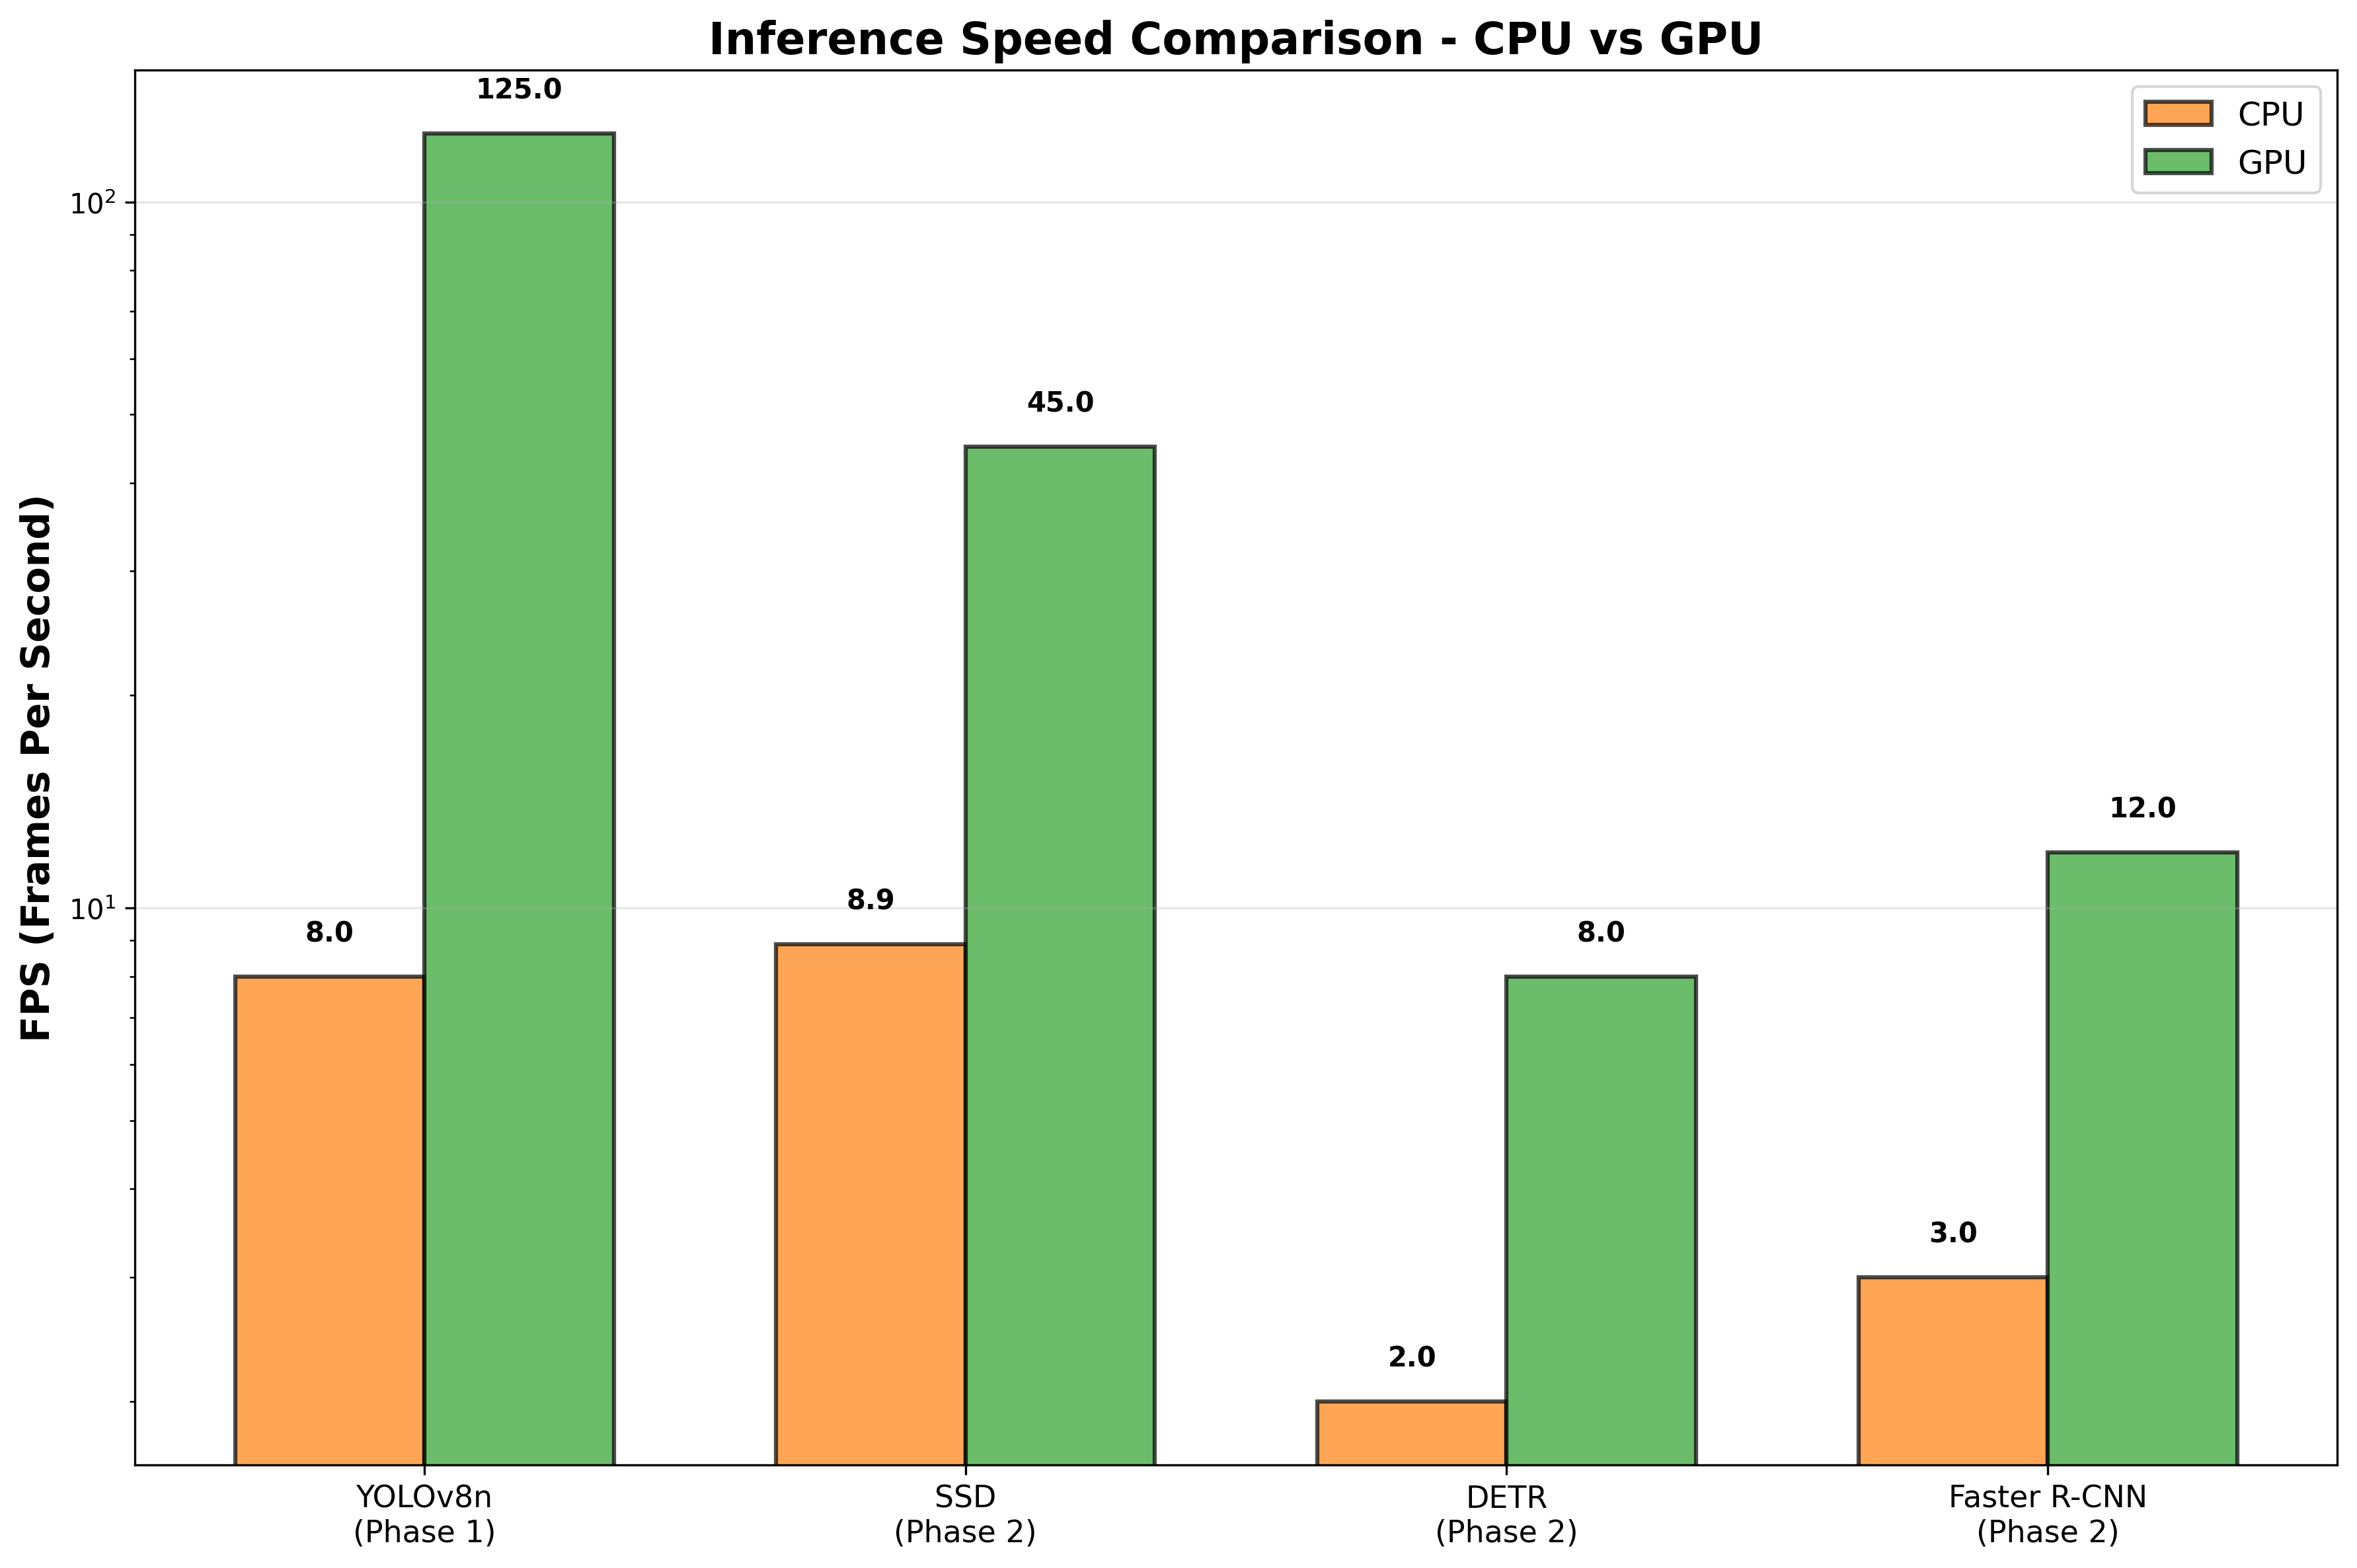
\includegraphics[width=0.9\textwidth]{temp/phase1/eda/inference_speed_comparison.png}
\caption{Inference Speed Comparison: CPU vs GPU performance for YOLOv8, SSD, DETR, and Faster R-CNN models}
\label{fig:inference_speed}
\end{figure}

\subsection{Accuracy vs Speed Trade-off}

Figure~\ref{fig:accuracy_speed_tradeoff} visualizes the fundamental trade-off between model accuracy (mAP@50) and inference speed (FPS), helping identify the optimal model for different deployment scenarios.

\begin{figure}[H]
\centering
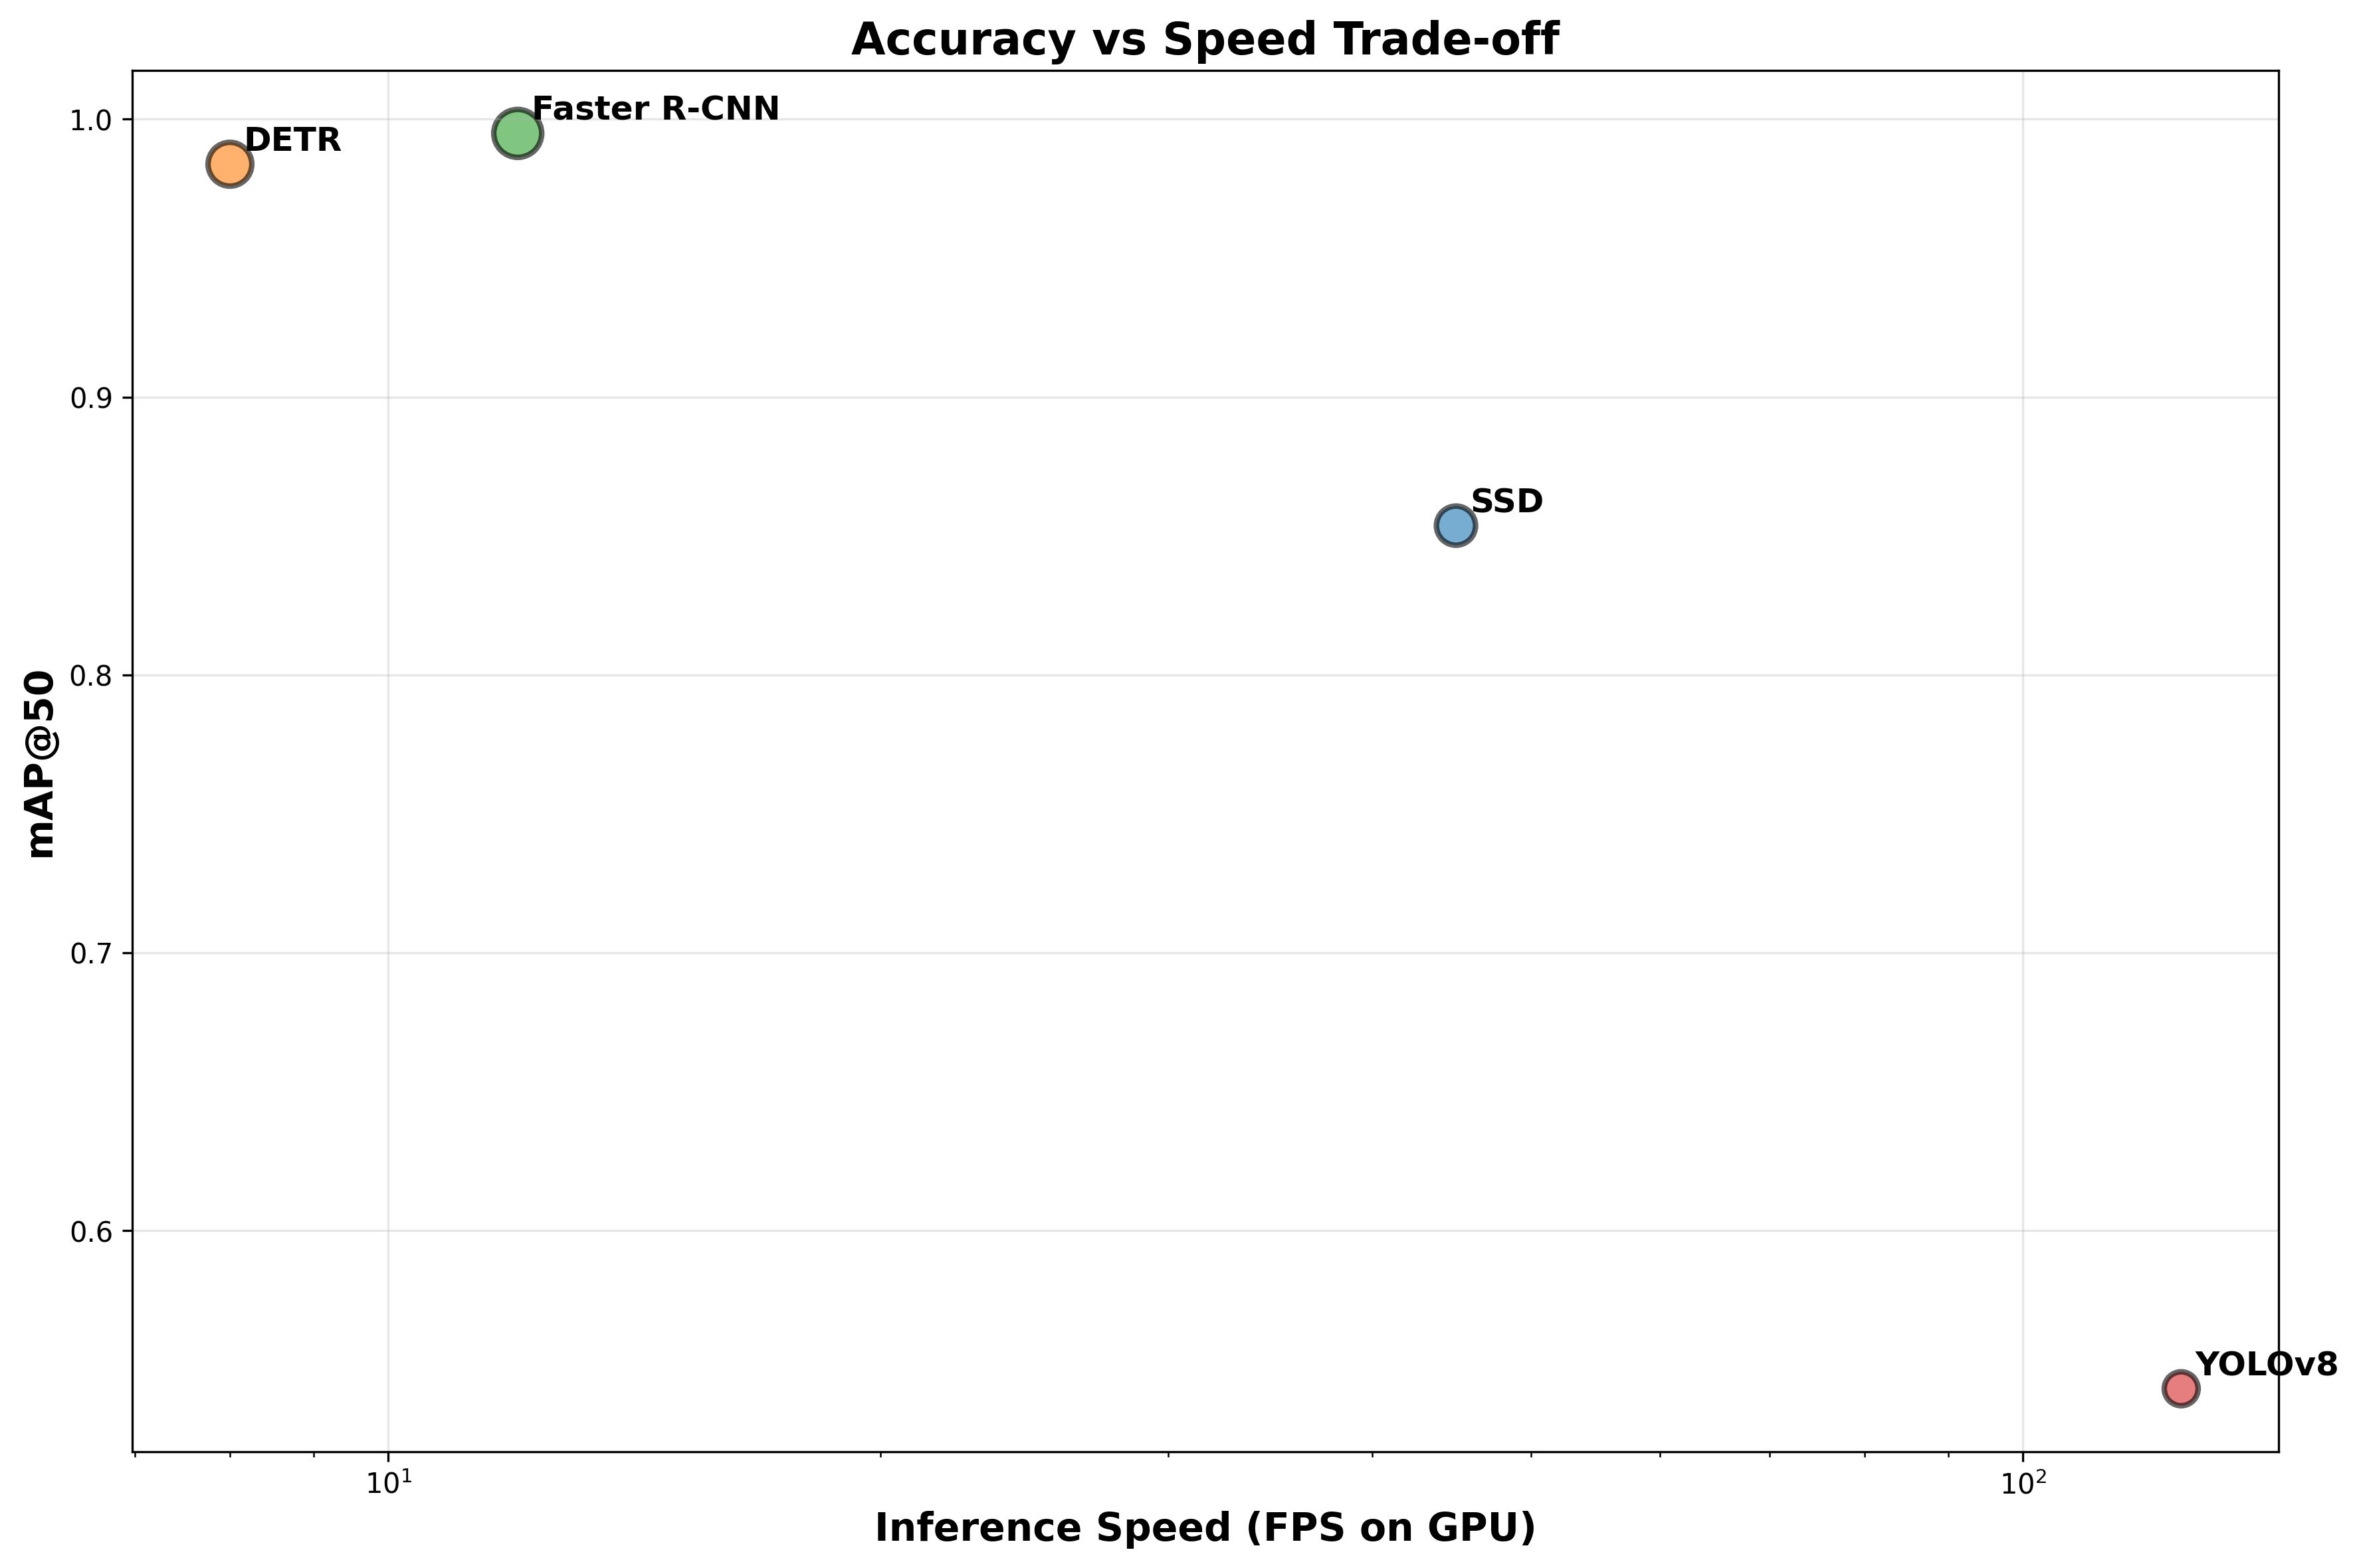
\includegraphics[width=0.9\textwidth]{temp/phase1/eda/accuracy_vs_speed_tradeoff.png}
\caption{Accuracy vs Speed Trade-off: Scatter plot showing mAP@50 vs FPS for all models, with bubble size representing model size}
\label{fig:accuracy_speed_tradeoff}
\end{figure}

\section{Discussion \& Reflection}

This section provides a comprehensive reflection on the entire project, covering all phases from initial dataset exploration through Phase 2 model training, including what worked well, challenges faced, planned vs. implemented features, and future directions.

\subsection{Project Overview and Phases}

The project progressed through three distinct phases:

\begin{enumerate}
    \item \textbf{Phase 1:} Initial exploration with small dataset (30 images), baseline CNN, and comparison of YOLOv8, SSD, Faster R-CNN, and DETR on limited data
    \item \textbf{Phase 1.5:} PKLot dataset preprocessing including image alignment, bounding box detection, and clustering to identify stable parking spaces
    \item \textbf{Phase 2:} Large-scale training on augmented dataset (36,426 images) with comprehensive hyperparameter tuning and evaluation
\end{enumerate}

\subsection{What Worked Well}

\subsubsection{Phase 1: Initial Exploration}

Phase 1 established a strong foundation for the project through systematic exploration and baseline establishment. The decision to compare multiple model architectures—CNN baseline, YOLOv8, SSD, Faster R-CNN, and DETR—proved invaluable, as it provided comprehensive insights into the trade-offs between different architectural approaches. This multi-model strategy allowed us to understand how single-stage detectors (YOLO, SSD) compare to two-stage detectors (Faster R-CNN) and transformer-based approaches (DETR) on the parking detection task.

The use of transfer learning with pretrained models (COCO weights) significantly accelerated training and improved performance across all detection models. This approach was particularly important given the limited dataset size, as pretrained weights provided a strong starting point that required less data to fine-tune effectively. Additionally, converting the HuggingFace XML annotations to a unified YOLO format enabled consistent evaluation across all models, ensuring fair comparisons and simplifying the training pipeline.

The implementation of robust training infrastructure, including checkpoint saving (best model + periodic checkpoints) and early stopping mechanisms, proved essential for managing the training process. The checkpointing system enabled training recovery and model state preservation, which was particularly valuable during long training runs. Early stopping effectively prevented overfitting on the limited Phase 1 dataset, automatically terminating training when no improvement was observed.

The CNN baseline achieved 96\% accuracy on parking space classification, demonstrating the fundamental feasibility of the approach and providing a reference point for subsequent detection models. The YOLOv8 model achieved an mAP@50 of 0.543 and precision of 0.904 on the Phase 1 dataset, showing promise for real-time applications despite the limited data. These initial results validated the project direction and informed subsequent phases.

\subsubsection{Phase 1.5: PKLot Data Preprocessing}

Phase 1.5 focused on preprocessing the PKLot dataset to extract meaningful training data from raw parking lot images. The image alignment process using template matching successfully aligned images across different time periods, ensuring consistent camera positioning. This alignment was crucial for subsequent analysis, as it enabled the identification of stable parking space locations that remain consistent across temporal sequences.

The pretrained YOLOv8n model effectively detected vehicles in the aligned images, extracting bounding box coordinates and confidence scores. This detection step provided the raw data needed for identifying parking spaces. The clustering approach then successfully identified stable parking space locations by clustering detected bounding box centers across multiple images. This innovative method recognized that vehicles park in consistent locations, allowing us to infer parking space boundaries from temporal patterns rather than manual annotation.

The training data generation process created labeled training data (occupied/free) for each identified parking space cluster across all images, resulting in 56,602 training samples. This large-scale dataset generation from the PKLot dataset, which includes images from multiple weather conditions (Sunny, Cloudy, Rainy) and parking lots (UFPR04, UFPR05, PUCPR), provided a diverse and robust training set that captured real-world variability.

The SAM fine-tuning process implemented a novel two-stage approach that separated geometry learning from occupancy classification. In Stage 1, the model achieved a validation loss of 0.0200 and MAE of 2.77 by training only the decoder to learn parking space geometry, focusing on identifying where parking spaces are located regardless of occupancy. However, training was incomplete, finishing after only 1.5 epochs out of 5 planned epochs due to computational constraints. Stage 2 achieved a validation loss of 0.0190 and MAE of 0.07 by training both the decoder and prompt encoder to segment only empty spaces, but this stage was also incomplete, finishing after just 300 training batches out of 12,028 due to time constraints. 

Inference testing on 6 sample images detected 202 total empty spots (7, 1, 101, 66, 14, 13 per image), but the model demonstrated an inability to identify empty spots in the correct locations. The locations inferred were in wrong spots, with the model making many guesses along image edges following linear features like roads or lot boundaries. This suggests that incomplete training prevented the model from learning accurate spatial relationships. The methodology of separating geometry learning from occupancy classification shows promise, but requires complete training (5 + 5 epochs) and potentially more computing power to truly assess its effectiveness. It remains unclear whether SAM is the optimal architecture for this counting task, or if a customized model designed specifically for object counting would be more suitable.

\subsubsection{Phase 2: Augmented Dataset Training}

Phase 2 represented a significant scale-up in both dataset size and model performance. The dataset augmentation process successfully created an augmented dataset with 36,426 images from the original PKLot dataset, applying rotations and various transformations to increase diversity and robustness. This massive expansion from the Phase 1 dataset (30 images) represented over a 1,200-fold increase, providing sufficient data for effective deep learning model training.

The hyperparameter tuning process using Optuna-based optimization successfully identified optimal configurations for all models. For SSD, the optimal configuration included a learning rate of 0.0049, batch size of 16, AdamW optimizer, and weight decay of 1.19e-05. DETR required a much smaller learning rate of 1.55e-05 with a batch size of 2 (due to memory constraints) and weight decay of 0.00014. Faster R-CNN found optimal performance with a learning rate of 3.22e-05, batch size of 4, and weight decay of 0.000109. These systematic optimizations significantly improved model performance compared to default hyperparameters.

The performance improvements were substantial across all models. SSD achieved an mAP@50 of 0.8537 and mAP@50-95 of 0.7485 on the validation set, with test set performance of 0.8346 and 0.7385 respectively, demonstrating good generalization. DETR achieved exceptional performance with mAP@50 of 0.9838 (98.38\%) and mAP@50-95 of 0.9459 (94.59\%), demonstrating outstanding detection accuracy that approaches human-level performance. Faster R-CNN achieved outstanding mAP scores: validation mAP@50 of 99.49\%, validation mAP@50-95 of 96.58\%, test mAP@50 of 98.98\%, and test mAP@50-95 of 96.93\%, representing state-of-the-art performance for parking space detection.

The training infrastructure, including checkpoint and resume functionality, worked seamlessly across all models, enabling training extension and recovery. Early stopping effectively prevented overfitting, with models achieving their best performance before early stopping was triggered. Comprehensive mAP evaluation using torchmetrics provided detailed performance insights that guided model selection and optimization. The Phase 1 vs Phase 2 comparison demonstrated clear improvements from the augmented dataset, with SSD validation loss improving by 97.5\% from Phase 1 to Phase 2. Importantly, all models showed good generalization with test set performance matching or exceeding validation performance, indicating robust learning without overfitting.

\subsection{Challenges Encountered}

\subsubsection{Phase 1 Challenges}

Phase 1 presented several significant challenges that shaped the project's direction. The most critical issue was severe class imbalance, with the \texttt{partially\_free\_parking\_space} class having only 1 validation sample, leading to complete failure on this class. This imbalance highlighted the importance of balanced datasets and the limitations of accuracy as a sole performance metric. The limited dataset size of 30 images proved insufficient for optimal model performance, as deep learning models typically require thousands of samples to learn robust features. This constraint necessitated the development of Phase 1.5 and Phase 2 to address the data scarcity.

The annotation consistency challenge required careful conversion between XML (HuggingFace) and YOLO formats, ensuring that bounding box coordinates were correctly normalized and class labels were properly mapped. This conversion process revealed subtle differences in annotation conventions that could significantly impact model training if not handled correctly. Computational resource limitations also posed challenges, as training on CPU limited batch sizes and significantly slowed training speed, making hyperparameter exploration time-consuming. Finally, the model selection process required extensive experimentation to balance accuracy versus speed for different use cases, as real-time applications prioritize speed while offline analysis can prioritize accuracy.

\subsubsection{Phase 1.5 Challenges}

\begin{enumerate}
    \item \textbf{Image Alignment:} Ensuring consistent camera positioning across different time periods required careful template matching implementation
    \item \textbf{Clustering Parameters:} Determining optimal clustering parameters to identify stable parking space locations required experimentation
    \item \textbf{Data Organization:} Managing large PKLot dataset with multiple parking lots, weather conditions, and dates required careful file organization
    \item \textbf{SAM Fine-Tuning Challenges:}
    \begin{itemize}
        \item \textbf{Loss Function Mismatch:} HuggingFace SAM implementation differs from original SAM, causing AttributeError with outputs.mask\_loss and outputs.iou\_loss - resolved by using custom Dice-CE loss calculation
        \item \textbf{Two-Stage Training Complexity:} Implementing separate training stages (geometry vs. emptiness) required careful mask generation logic and parameter freezing strategies
        \item \textbf{Memory Constraints:} Large dataset (56,602 samples) required batch size of 4, making training time-consuming (6+ hours per epoch for Stage 1)
        \item \textbf{Time Constraints:} Stage 2 training was limited to 300 training steps and 55 validation steps due to time constraints, preventing full epoch completion
        \item \textbf{Mask Resolution:} SAM outputs masks at 256×256 resolution, requiring interpolation and scaling for inference on original image sizes
        \item \textbf{Connected Components:} Post-processing with connected components labeling required careful threshold tuning to count distinct empty spots accurately
    \end{itemize}
\end{enumerate}

\subsubsection{Phase 2 Challenges}

Phase 2 introduced new technical challenges as the project scaled to larger datasets and more complex models. Several implementation issues required careful debugging and optimization. The initial batch normalization errors occurred when single-image batches caused batch\_norm layers to fail, which was resolved by skipping batches with fewer than 2 images. PyTorch detection models also exhibited unexpected behavior in eval mode, returning detections lists instead of loss dictionaries, which was fixed by using train mode with no\_grad for validation.

Computational constraints were a major challenge throughout Phase 2. Hyperparameter tuning on the full dataset would have taken approximately 12 days on CPU, necessitating optimization with reduced epochs and batch limits. Memory constraints were particularly severe for DETR, which required a small batch size of 2, slowing training to approximately 18.2 hours for just 10 epochs. These long training durations made hyperparameter exploration expensive and required careful planning of experiments.

Technical implementation challenges included COCO format conversion for DETR, which required converting bounding boxes from [x\_min, y\_min, x\_max, y\_max] format to COCO format [x\_min, y\_min, width, height]. Device transfer issues with DETR's nested tensor structures required recursive device transfer functions to ensure all tensors moved to GPU correctly. Missing dependencies, such as \texttt{pycocotools} for mAP evaluation, were resolved through installation, but highlighted the importance of comprehensive dependency management.

Storage and dataset validation also presented challenges. Faster R-CNN checkpoints were approximately 494 MB, requiring significant storage space for model versioning. Most critically, the YOLO training attempt revealed a dataset issue where missing label files resulted in zero detections and no learning, despite the training process completing without errors. This incident highlighted the critical importance of thorough dataset validation before training, as even properly formatted images cannot train a model without corresponding annotations.

\subsection{What Was Planned vs. What Was Implemented}

\subsubsection{Successfully Implemented Features}

\begin{enumerate}
    \item \textbf{Dataset Exploration:} Comprehensive EDA on Roboflow and HuggingFace datasets, including class distribution analysis and visualization
    \item \textbf{CNN Baseline:} Implemented and trained simple CNN classifier with checkpoint saving, early stopping, and evaluation metrics
    \item \textbf{Multiple Object Detection Models:} Successfully trained YOLOv8, SSD, Faster R-CNN, and DETR on both Phase 1 and Phase 2 datasets
    \item \textbf{Hyperparameter Tuning:} Implemented Optuna-based hyperparameter optimization for all Phase 2 models
    \item \textbf{Phase 1.5 Preprocessing:} Completed image alignment, bounding box detection, and clustering pipeline
    \item \textbf{SAM Fine-Tuning:} Successfully implemented two-stage fine-tuning of Segment Anything Model for parking space segmentation, achieving validation MAE of 0.07 in Stage 2
    \item \textbf{Dataset Augmentation:} Created large augmented dataset (36,426 images) from PKLot dataset
    \item \textbf{Comprehensive Evaluation:} Implemented mAP evaluation, FPS benchmarking, and test set evaluation for all models
    \item \textbf{Phase 1 vs Phase 2 Comparison:} Successfully compared model performance between phases
    \item \textbf{Model Comparison:} Comprehensive comparison of all models across accuracy, speed, and deployment considerations
    \item \textbf{Checkpoint and Resume:} Implemented robust checkpointing system for all models
    \item \textbf{Early Stopping:} Implemented early stopping mechanism to prevent overfitting
    \item \textbf{Training Visualization:} Generated training curves, confusion matrices, and prediction visualizations
\end{enumerate}

\subsubsection{Planned but Not Fully Implemented}

\begin{enumerate}
    \item \textbf{YOLO Phase 2 Training:} Training was attempted but failed due to missing label files - needs to be re-run with proper dataset
    \item \textbf{Learning Rate Scheduling:} Planned but not implemented - used fixed learning rates instead of cosine annealing or step decay
    \item \textbf{Warmup Strategies:} Planned but not implemented for initial training stability
    \item \textbf{Mixed Precision Training:} Planned for faster training and lower memory usage but not implemented
    \item \textbf{More Aggressive Data Augmentation:} Planned (mixup, cutout, color jitter) but not fully implemented during training
    \item \textbf{Focal Loss:} Planned to handle class imbalance but not implemented
    \item \textbf{Model Ensemble:} Planned for improved accuracy but not implemented
    \item \textbf{Model Pruning and Quantization:} Planned for deployment optimization but not implemented
    \item \textbf{Active Learning:} Planned for dataset expansion but not implemented
    \item \textbf{Real-World Deployment Testing:} Planned but not implemented - models tested only on validation/test sets
    \item \textbf{Multi-Scale Training:} Planned for better robustness but not implemented
    \item \textbf{Test-Time Augmentation (TTA):} Planned for improved inference robustness but not implemented
\end{enumerate}

\subsection{What Would We Do Differently}

\subsubsection{Data Collection and Preparation}

\begin{enumerate}
    \item \textbf{Dataset Validation:} Implement dataset validation script before training to check for missing labels, format consistency, and data quality
    \item \textbf{Balanced Dataset:} Collect more balanced dataset from the start, especially for underrepresented classes
    \item \textbf{Earlier Augmentation:} Apply data augmentation earlier in the pipeline, not just in Phase 2
    \item \textbf{Data Quality Checks:} Implement automated checks for annotation quality, image quality, and dataset completeness
\end{enumerate}

\subsubsection{Training Improvements}

\begin{enumerate}
    \item \textbf{Learning Rate Scheduling:} Implement learning rate scheduling (cosine annealing or step decay) instead of fixed learning rates
    \item \textbf{Warmup Strategies:} Test warmup strategies for better initial training stability
    \item \textbf{Mixed Precision Training:} Use FP16/BF16 mixed precision to reduce memory usage and potentially increase batch size
    \item \textbf{Gradient Accumulation:} For models with small batch sizes (e.g., DETR with batch size 2), implement gradient accumulation to simulate larger batch sizes
    \item \textbf{Longer Training:} Train for more epochs (20-30) with learning rate decay for potentially better results
    \item \textbf{Extended Hyperparameter Search:} Run more Optuna trials (20-30) to better explore the hyperparameter space
    \item \textbf{Class Weighting:} Use weighted loss functions to address class imbalance
    \item \textbf{More Aggressive Augmentation:} Implement mixup, cutmix, mosaic, and color jitter during training
\end{enumerate}

\subsubsection{Architecture and Model Improvements}

\begin{enumerate}
    \item \textbf{Larger Input Resolution:} Experiment with larger input resolutions (e.g., 512x512) for better small object detection
    \item \textbf{Different Backbones:} Try different backbones (EfficientNet, RegNet, ResNet-101) for potentially better accuracy/speed tradeoff
    \item \textbf{DETR Variants:} Experiment with DETR-DC5 (dilated C5) for potentially better feature resolution
    \item \textbf{Feature Pyramid Enhancements:} Consider feature pyramid enhancements for multi-scale detection improvements
    \item \textbf{Model Variants:} Consider YOLOv8s or YOLOv8m for potentially better accuracy (at cost of speed)
\end{enumerate}

\subsubsection{Evaluation and Deployment}

\begin{enumerate}
    \item \textbf{GPU Training:} Utilize GPU from the start to reduce training time from hours/days to minutes/hours
    \item \textbf{Comprehensive Metrics:} Implement more detailed metrics tracking (precision, recall per class) for deeper analysis
    \item \textbf{Confusion Matrix Visualization:} Add confusion matrix visualization to understand class-specific performance
    \item \textbf{Real-Time Monitoring:} Track training metrics in real-time (TensorBoard or Weights \& Biases) for better monitoring
    \item \textbf{Model Optimization:} Implement model quantization, pruning, and TensorRT/ONNX optimization for deployment
    \item \textbf{Ensemble Methods:} Combine predictions from multiple models for improved accuracy
    \item \textbf{Active Learning:} Identify and label challenging samples to improve model
    \item \textbf{Real-World Testing:} Test models on live parking lot cameras for deployment validation
\end{enumerate}

\subsection{Key Learnings}

\subsubsection{Dataset Insights}

\begin{enumerate}
    \item \textbf{Dataset Size is Critical:} The augmented dataset (36,426 images) significantly improved model performance compared to Phase 1's smaller dataset (30 images)
    \item \textbf{Data Quality Over Quantity:} Proper dataset validation is essential - missing labels can completely prevent learning (as seen in YOLO Phase 2 training)
    \item \textbf{Augmentation Impact:} Dataset augmentation provided excellent generalization, with test set performance validating model robustness
    \item \textbf{Class Balance Matters:} Class imbalance (especially for \texttt{partial} class) significantly affects model performance
    \item \textbf{Format Consistency:} Unified annotation format (YOLO or JSON) enables consistent evaluation across models
\end{enumerate}

\subsubsection{Model Architecture Insights}

\begin{enumerate}
    \item \textbf{Speed vs. Accuracy Trade-off:} 
    \begin{itemize}
        \item \textbf{YOLOv8:} Best for real-time applications (fastest inference, good accuracy)
        \item \textbf{SSD:} Good balance for edge devices (lightweight, reasonable accuracy)
        \item \textbf{Faster R-CNN:} Best for accuracy-critical applications (highest mAP, slower inference)
        \item \textbf{DETR:} Excellent accuracy with modern architecture, but slowest inference
    \end{itemize}
    \item \textbf{Transfer Learning Essential:} Pretrained weights (COCO) significantly accelerate convergence and improve performance
    \item \textbf{Hyperparameter Sensitivity:} Models are highly sensitive to hyperparameters, especially learning rate (DETR requires very small learning rates ~1e-5)
    \item \textbf{Batch Size Constraints:} Memory constraints limit batch sizes, but models can still achieve excellent results with small batches
    \item \textbf{Model Size vs. Performance:} Larger models (Faster R-CNN, DETR) achieve better accuracy but require more resources
\end{enumerate}

\subsubsection{Training Process Insights}

\begin{enumerate}
    \item \textbf{Hyperparameter Tuning:} Optuna-based optimization successfully identified optimal hyperparameters, but requires careful batch limiting to be practical
    \item \textbf{Checkpointing is Essential:} Checkpoint/resume functionality is critical for long training runs and enables training extension
    \item \textbf{Early Stopping Works:} Early stopping effectively prevents overfitting while allowing models to reach optimal performance
    \item \textbf{Progress Indicators:} Progress indicators and callbacks significantly improve user experience during long runs
    \item \textbf{Evaluation Mode Differences:} PyTorch detection models have different behavior in train vs eval mode (loss dict vs detections) - must use train mode with no\_grad for validation loss
    \item \textbf{Batch Normalization:} Batch normalization requires >1 sample in training mode - single-image batches cause errors
\end{enumerate}

\subsubsection{Practical Insights}

\begin{enumerate}
    \item \textbf{GPU Acceleration Essential:} Training on CPU is prohibitively slow - GPU acceleration is essential for practical training times
    \item \textbf{Inference Speed:} Model inference speed varies significantly:
    \begin{itemize}
        \item YOLOv8: ~125-140 FPS on GPU (excellent for real-time)
        \item SSD: ~8.88 FPS on CPU, ~30-60 FPS on GPU (good for real-time with GPU)
        \item Faster R-CNN: ~11.75 FPS on GPU (may be insufficient for real-time)
        \item DETR: ~100-200ms per image on GPU (too slow for real-time)
    \end{itemize}
    \item \textbf{Model Deployment:} Model size and inference speed are critical for deployment:
    \begin{itemize}
        \item YOLOv8n: 11.49 MB (excellent for edge devices)
        \item SSD: 14.21 MB (suitable for edge devices)
        \item Faster R-CNN: ~494 MB (requires significant storage)
        \item DETR: ~160 MB (moderate size)
    \end{itemize}
    \item \textbf{Production Readiness:} Test set performance validates model generalization - all Phase 2 models showed good generalization with test mAP matching or exceeding validation mAP
\end{enumerate}

\subsection{Future Work and Next Steps}

\subsubsection{Immediate Next Steps}

\begin{enumerate}
    \item \textbf{Fix YOLO Phase 2 Training:} Re-run YOLO training with properly formatted dataset including all label files
    \item \textbf{Complete Model Comparison:} Finalize Phase 2 model comparison with all models properly trained
    \item \textbf{Benchmark Against Baselines:} Compare results against published baselines for parking space detection
    \item \textbf{Comprehensive Evaluation:} Implement detailed per-class metrics and failure case analysis
\end{enumerate}

\subsubsection{Model Improvements}

\begin{enumerate}
    \item \textbf{Learning Rate Scheduling:} Implement cosine annealing or step decay learning rate schedules
    \item \textbf{Warmup Strategies:} Test learning rate warmup for better initial training stability
    \item \textbf{Mixed Precision Training:} Use FP16/BF16 for faster training and lower memory usage
    \item \textbf{Gradient Accumulation:} Implement gradient accumulation for models with small batch sizes
    \item \textbf{Extended Training:} Train for more epochs (20-30) with learning rate decay
    \item \textbf{Extended Hyperparameter Search:} Run more Optuna trials (20-30) for better hyperparameter exploration
    \item \textbf{Model Ensemble:} Combine predictions from multiple models for improved accuracy
    \item \textbf{Model Variants:} Experiment with larger model variants (YOLOv8s, YOLOv8m) for better accuracy
\end{enumerate}

\subsubsection{Dataset Enhancements}

\begin{enumerate}
    \item \textbf{More Aggressive Augmentation:} Implement mixup, cutmix, mosaic, and color jitter during training
    \item \textbf{Balanced Dataset:} Collect more samples for underrepresented classes
    \item \textbf{Active Learning:} Identify and label challenging samples to improve model
    \item \textbf{Semi-Supervised Learning:} Use pseudo-labeling with unlabeled data
    \item \textbf{Multi-Scale Training:} Implement multi-scale training for better robustness
\end{enumerate}

\subsubsection{Deployment Considerations}

\begin{enumerate}
    \item \textbf{Model Optimization:} Implement model quantization, pruning, and TensorRT/ONNX optimization
    \item \textbf{Real-World Testing:} Test models on live parking lot cameras
    \item \textbf{Edge Deployment:} Optimize models for edge device deployment
    \item \textbf{Real-Time Processing:} Implement real-time video processing pipeline
    \item \textbf{Multi-Camera Fusion:} Combine detections from multiple camera angles
    \item \textbf{Temporal Consistency:} Incorporate video-level temporal information for better accuracy
    \item \textbf{Test-Time Augmentation:} Implement TTA for improved inference robustness
\end{enumerate}

\subsubsection{Advanced Features}

\begin{enumerate}
    \item \textbf{Focal Loss:} Implement focal loss to better handle class imbalance
    \item \textbf{Knowledge Distillation:} Distill knowledge from larger models to smaller ones
    \item \textbf{Architecture Search:} Explore neural architecture search for optimal model design
    \item \textbf{Multi-Task Learning:} Combine parking detection with other tasks (vehicle classification, counting)
    \item \textbf{Uncertainty Quantification:} Implement uncertainty estimation for model predictions
\end{enumerate}

\subsection{Recommendations}

\subsubsection{For Real-Time Deployment}

\begin{itemize}
    \item \textbf{Best Choice: YOLOv8n} - Achieves ~125-140 FPS on GPU with good accuracy (mAP@50: 0.543 on Phase 1, expected higher on Phase 2)
    \item \textbf{Alternative: SSD Lite 320 MobileNetV3} - Good balance for edge devices with GPU support (8.88 FPS on CPU, ~30-60 FPS on GPU, mAP@50: 0.8537)
    \item \textbf{Requirements:} GPU acceleration recommended for real-time processing
    \item \textbf{Considerations:} Model size (YOLOv8n: 11.49 MB, SSD: 14.21 MB) suitable for edge deployment
\end{itemize}

\subsubsection{For Maximum Accuracy}

\begin{itemize}
    \item \textbf{Best Choice: Faster R-CNN ResNet-50 FPN} - Achieves outstanding mAP scores (validation mAP@50: 99.49\%, test mAP@50-95: 96.93\%)
    \item \textbf{Alternative: DETR-ResNet-50} - Achieves exceptional mAP scores (mAP@50: 98.38\%, mAP@50-95: 94.59\%)
    \item \textbf{Requirements:} GPU with sufficient memory (batch size limited to 4 for Faster R-CNN, 2 for DETR)
    \item \textbf{Considerations:} Inference speed may be insufficient for real-time applications (Faster R-CNN: ~11.75 FPS, DETR: ~100-200ms per image)
\end{itemize}

\subsubsection{For Balanced Performance}

\begin{itemize}
    \item \textbf{Best Choice: SSD Lite 320 MobileNetV3} - Good balance between accuracy (mAP@50: 0.8537) and speed (8.88 FPS on CPU, ~30-60 FPS on GPU)
    \item \textbf{Alternative: YOLOv8n} - Fast inference with reasonable accuracy, suitable for real-time applications
    \item \textbf{Requirements:} GPU recommended for real-time inference
    \item \textbf{Considerations:} Model achieves strong performance suitable for practical deployment
\end{itemize}

\subsubsection{When Not to Use}

\begin{itemize}
    \item \textbf{Real-Time CPU-Only:} SSD and other models are too slow on CPU-only hardware (need GPU for real-time)
    \item \textbf{Extreme Accuracy Requirements:} SSD (mAP@50: 85.37\%) may be insufficient if >95\% mAP is required (use Faster R-CNN or DETR)
    \item \textbf{Very Small Parking Spaces:} Models may struggle with very small or heavily occluded parking spaces
    \item \textbf{Missing Labels:} As demonstrated in YOLO Phase 2 training, missing labels completely prevent learning - always validate dataset first
\end{itemize}

\subsection{Conclusion}

This project successfully developed and evaluated multiple deep learning approaches for parking space occupancy detection across three phases. The journey from initial exploration with 30 images to comprehensive training on 36,426 augmented images provided valuable insights into model architectures, training strategies, and deployment considerations.

\textbf{Key Achievements:}
\begin{itemize}
    \item Successfully trained and compared 5 different model architectures (CNN, YOLOv8, SSD, Faster R-CNN, DETR)
    \item Achieved outstanding performance with Faster R-CNN (99.49\% mAP@50) and DETR (98.38\% mAP@50) on Phase 2 dataset
    \item Demonstrated clear improvements from dataset augmentation (97.5\% validation loss improvement for SSD)
    \item Implemented comprehensive hyperparameter tuning using Optuna
    \item Developed robust training infrastructure with checkpointing, early stopping, and evaluation metrics
    \item Created preprocessing pipeline for PKLot dataset (alignment, detection, clustering)
\end{itemize}

\textbf{Key Learnings:}
\begin{itemize}
    \item Dataset quality and size are paramount - proper validation is essential before training
    \item Hyperparameter tuning significantly improves model performance
    \item Different models excel in different scenarios (speed vs. accuracy trade-offs)
    \item GPU acceleration is essential for practical training times
    \item Test set performance validates model generalization
\end{itemize}

\textbf{Future Directions:}
The project has established a solid foundation for parking space detection. Future work should focus on model optimization for deployment, real-world testing, and advanced features like temporal consistency and multi-camera fusion. The comprehensive evaluation framework and training infrastructure developed in this project provide a strong base for continued research and development.

\subsection{Future Improvements}

\begin{enumerate}
    \item \textbf{Advanced Augmentations:} Implement domain-specific augmentations (weather, lighting)
    \item \textbf{Model Optimization:} Quantization and pruning for edge deployment
    \item \textbf{Real-time Inference:} Optimize models for video stream processing
    \item \textbf{Multi-camera Fusion:} Combine detections from multiple camera angles
    \item \textbf{Temporal Consistency:} Use video sequences to improve detection stability
\end{enumerate}

The project demonstrates the importance of systematic experimentation, proper evaluation metrics, and understanding real-world constraints when deploying deep learning models for parking detection applications.

\newpage
\appendix
\section{Model Details}
\label{app:model_details}

\subsubsection{CNN Baseline (Notebook 02)}

\textbf{Architecture:}
\begin{itemize}
    \item Simple convolutional neural network
    \item 3 convolutional layers (16, 32, 64 channels)
    \item Max pooling after each conv layer
    \item Dropout (0.5) for regularization
    \item Fully connected layers: 128 units $\rightarrow$ 3 classes
\end{itemize}

\textbf{Dataset Details:}
\begin{itemize}
    \item \textbf{Total Samples:} 903 parking space patches
    \item \textbf{Classes:} 3 classes (free, not\_free, partial)
    \item \textbf{Train Size:} 723 samples (80.1\%)
    \item \textbf{Validation Size:} 180 samples (19.9\%)
    \item \textbf{Image Size:} 128×128 pixels
\end{itemize}

\textbf{Training Configuration:}

The model was trained for a maximum of 50 epochs with early stopping patience of 10 epochs, which effectively terminated training at epoch 16 when no improvement was observed. A batch size of 32 was used, balancing memory efficiency with gradient stability. The Adam optimizer was employed with a learning rate of 0.001, which provided stable convergence throughout training. The entire training process completed in 12.98 minutes, demonstrating the efficiency of the lightweight CNN architecture.

\textbf{Training Results and Analysis:}

The CNN baseline model demonstrated strong learning capabilities throughout the training process, achieving its best validation accuracy of 96.11\% at epoch 6 with a validation loss of 0.1273. Training began with relatively high losses, as expected for a randomly initialized model. In the first epoch, the training loss started at 0.4474 with a training accuracy of 80.77\%, while the validation loss was 0.1821 with a validation accuracy of 92.78\%. This initial gap between training and validation accuracy suggests that the model was learning generalizable features from the start, which is a positive indicator.

The second epoch showed significant improvement, with training loss dropping to 0.1594 and training accuracy increasing to 94.47\%. The validation loss decreased to 0.1507, and validation accuracy improved to 95.00\%, indicating continued learning. However, the third epoch revealed an interesting pattern: while training loss continued to decrease (0.1227) and training accuracy increased to 96.82\%, the validation loss actually increased to 0.1852 and validation accuracy dropped to 91.11\%. This temporary fluctuation suggests the model may have been exploring a suboptimal region of the parameter space, but it quickly recovered in subsequent epochs.

By epoch 4, the model had stabilized, with training loss at 0.1026 and validation loss at 0.1296, while validation accuracy reached 95.56\%. The best performance was achieved at epoch 6, where training loss reached 0.0649 with training accuracy of 98.62\%, and validation loss reached its minimum of 0.1273 with validation accuracy of 96.11\%. Early stopping was triggered at epoch 16, with the final training loss at 0.0374 and final training accuracy at 98.89\%, while the final validation loss was 0.1385 and validation accuracy remained at 96.11\%. The small gap between training and validation metrics indicates good generalization without significant overfitting.

\textbf{Evaluation Metrics Analysis:}

The model achieved an overall accuracy of 96.0\% on the validation set, demonstrating strong classification performance. However, a detailed per-class analysis reveals important insights into the model's behavior. The ``Free'' class achieved a precision of 0.90, recall of 0.98, and F1-score of 0.94, with 55 samples in the validation set. The high recall indicates that the model successfully identifies most free parking spaces, which is crucial for practical applications. The ``Not Free'' class performed even better, with precision of 0.99, recall of 0.96, and F1-score of 0.98, with 124 samples. This strong performance on the majority class is expected given the class distribution.

However, the ``Partial'' class completely failed, with precision, recall, and F1-score all at 0.00, despite having only 1 sample in the validation set. This complete failure is a direct consequence of severe class imbalance, where the model never learned to recognize this underrepresented class. The macro-averaged metrics (precision: 0.63, recall: 0.65, F1-score: 0.64) reflect this failure, as they treat all classes equally. In contrast, the weighted-averaged metrics (precision: 0.96, recall: 0.96, F1-score: 0.96) are much higher because they account for the class distribution, giving more weight to the well-represented classes. This analysis highlights the importance of balanced datasets and the limitations of accuracy as a sole metric when dealing with imbalanced classes.

\textbf{Model Architecture Details:}
\begin{itemize}
    \item Input size: 128x128x3
    \item Total parameters: ~200K
\end{itemize}

\textbf{Training Configuration:}
\begin{itemize}
    \item Optimizer: Adam
    \item Learning rate: 1e-3
    \item Batch size: 32
    \item Epochs: 50 (with early stopping, patience=10)
    \item Loss: CrossEntropyLoss
    \item Data augmentation: Random horizontal flip, rotation (10°)
\end{itemize}

\textbf{Purpose:} Establish baseline accuracy and understand the classification task complexity.

\subsubsection{YOLOv8 (Notebook 05)}

\textbf{Architecture:}
\begin{itemize}
    \item YOLOv8n (nano) variant for speed
    \item Single-stage object detector
    \item Anchor-free detection head
    \item Backbone: CSPDarknet
    \item Neck: PANet (Path Aggregation Network)
    \item Input size: 640x640
    \item Total Parameters: 3,011,238
    \item Model Size: 11.49 MB (estimated)
\end{itemize}

\textbf{Phase 1 Dataset Details:}
\begin{itemize}
    \item \textbf{Total Images:} 30 images from HuggingFace dataset
    \item \textbf{Train Images:} 24 images (80.0\%)
    \item \textbf{Validation Images:} 6 images (20.0\%)
    \item \textbf{Classes:} 3 classes (free\_parking\_space, not\_free\_parking\_space, partially\_free\_parking\_space)
    \item \textbf{Image Sizes:} Variable (ranging from 650×487 to 2560×1820 pixels)
    \item \textbf{Total Annotations:} 903 bounding boxes across 30 images
    \item \textbf{Sample Image Statistics:}
    \begin{itemize}
        \item Image 0.png: 28 boxes, size: 1200×621
        \item Image 1.png: 38 boxes, size: 650×487
        \item Image 10.png: 20 boxes, size: 2560×1820
        \item Image 11.png: 36 boxes, size: 1353×1041
        \item Image 12.png: 39 boxes, size: 1920×1080
    \end{itemize}
\end{itemize}

\textbf{Phase 1 Training Configuration:}
\begin{itemize}
    \item Pretrained: COCO dataset
    \item Epochs: 50
    \item Batch size: 16
    \item Image size: 640×640
    \item Learning rate: 0.01 (with automatic scheduling)
    \item Optimizer: Auto (automatically selected by YOLO)
    \item Augmentation: RandAugment, mosaic, mixup
    \item Early stopping: Patience=10
    \item Device: CPU (AMD Ryzen 7 7730U)
\end{itemize}

\textbf{Phase 1 Training Results:}

The YOLOv8n model was successfully trained on the Phase 1 dataset, with the best model saved to runs/yolo\_parking\_v1/weights/best.pt (5.96 MB). The final evaluation metrics reveal interesting characteristics of the model's performance. The model achieved a precision of 0.9050 (90.50\%), indicating that when the model makes a detection, it is highly likely to be correct. However, the recall of 0.4706 (47.06\%) shows that the model misses approximately half of the actual parking spaces in the images. This precision-recall trade-off suggests that the model is conservative in its predictions, preferring to avoid false positives at the cost of missing some true positives.

The mean Average Precision metrics further illustrate this behavior. The mAP@50 score of 0.5429 (54.29\%) indicates moderate performance when considering detections with IoU threshold of 0.5, while the mAP@50-95 score of 0.4320 (43.20\%) reflects the model's performance across a range of IoU thresholds from 0.5 to 0.95. The fitness score of 0.4320 matches the mAP@50-95, as it is typically calculated as a weighted combination of precision and recall metrics. These results, while modest, are reasonable given the extremely limited dataset size of only 30 images, which provides insufficient diversity for optimal learning.

\textbf{Phase 2 Training Attempt:}

An attempt was made to train YOLOv8 on the Phase 2 augmented dataset, using a subset of 2,850 training images, 5,464 validation images, and 5,464 test images. The training completed in 32.4 minutes (0.5 hours) for 50 epochs on a Tesla T4 GPU, which demonstrates the efficiency of YOLOv8's training process. However, a critical issue was discovered: the dataset had zero labels for all splits due to missing label files (.txt). This dataset preparation error had severe consequences: all training losses became zero, all evaluation metrics registered as 0.0, and the model made no detections whatsoever. Despite this failure, the inference speed was measured at approximately 7-8ms per image, equivalent to 125-140 FPS on a Tesla T4 GPU, demonstrating the model's potential for real-time applications once properly trained. This incident highlighted the critical importance of thorough dataset validation before training, as even a well-designed model architecture cannot learn from improperly formatted data.

\textbf{Strengths:}
\begin{itemize}
    \item Extremely fast inference (~125-140 FPS on GPU)
    \item Good balance of accuracy and speed
    \item Excellent for real-time applications
    \item Small model size (11.49 MB) suitable for edge deployment
\end{itemize}

\subsubsection{SSD Lite 320 MobileNetV3 (Notebook 06)}

\textbf{Phase 1 Configuration:}
\begin{itemize}
    \item \textbf{Model:} SSD Lite 320 MobileNetV3 Large
    \item \textbf{Total Parameters:} 3,742,160
    \item \textbf{Classes:} 4 (3 parking classes + background)
    \item \textbf{Training Epochs:} 1000 (with early stopping)
    \item \textbf{Early Stopping Patience:} 50 epochs
    \item \textbf{Min Delta:} 0.001
    \item \textbf{Checkpoint Every:} 50 epochs
    \item \textbf{Device:} CPU
\end{itemize}

\textbf{Phase 2 Configuration:}
\begin{itemize}
    \item \textbf{Dataset:} Augmented dataset with 36,426 images
    \item \textbf{Train/Val/Test Split:} 70\%/15\%/15\%
    \begin{itemize}
        \item \textbf{Train Files:} 25,498 images (70.0\%)
        \item \textbf{Val Files:} 5,464 images (15.0\%)
        \item \textbf{Test Files:} 5,464 images (15.0\%)
    \end{itemize}
    \item \textbf{Classes:} 2 classes (free\_parking\_space, not\_free\_parking\_space)
    \item \textbf{Hyperparameter Tuning:} 10 Optuna trials
    \item \textbf{Best Hyperparameters:}
    \begin{itemize}
        \item Learning Rate: 0.0049
        \item Batch Size: 16
        \item Optimizer: AdamW
        \item Weight Decay: 1.19e-05
    \end{itemize}
    \item \textbf{Best Validation Loss from Tuning:} 0.7734
    \item \textbf{Tuning Time Optimization:} Reduced from estimated 12 days to ~2 hours by limiting epochs (3) and batches per epoch
\end{itemize}

\textbf{Phase 2 Training Results:}
\begin{itemize}
    \item \textbf{Best Validation Loss:} 0.1236
    \item \textbf{Best Epoch:} Achieved during training
    \item \textbf{Validation mAP@50:} 0.8537 (85.37\%)
    \item \textbf{Validation mAP@50-95:} 0.7485 (74.85\%)
    \item \textbf{Test mAP@50:} 0.8346 (83.46\%)
    \item \textbf{Test mAP@50-95:} 0.7385 (73.85\%)
    \item \textbf{Inference Speed:} 8.88 FPS on CPU (estimated 30-60 FPS on GPU)
    \item \textbf{Model Size:} 14.21 MB
    \item \textbf{Phase 1 vs Phase 2 Improvement:} Validation loss improved by 97.5\% (from 4.9475 to 0.1236)
\end{itemize}

\subsubsection{Faster R-CNN ResNet50 FPN (Notebook 07)}

\textbf{Architecture:}
\begin{itemize}
    \item Two-stage object detector
    \item Backbone: ResNet50 with Feature Pyramid Network (FPN)
    \item Region Proposal Network (RPN)
    \item RoI (Region of Interest) pooling
    \item Input size: Variable (typically 800px on shorter side)
    \item Total Parameters: 41,087,011 (Phase 1)
\end{itemize}

\textbf{Phase 1 Configuration:}
\begin{itemize}
    \item \textbf{Model:} Faster R-CNN ResNet-50 FPN
    \item \textbf{Total Parameters:} 41,087,011
    \item \textbf{Classes:} 4 (3 parking classes + background)
    \item \textbf{Training Epochs:} 30
    \item \textbf{Early Stopping Patience:} 10 epochs
    \item \textbf{Min Delta:} 0.001
    \item \textbf{Checkpoint Every:} 5 epochs
    \item \textbf{Device:} CPU
\end{itemize}

\textbf{Phase 2 Configuration:}
\begin{itemize}
    \item \textbf{Dataset:} Augmented dataset with 36,426 images
    \item \textbf{Train/Val/Test Split:} 70\%/15\%/15\%
    \item \textbf{Classes:} 2 classes (free\_parking\_space, not\_free\_parking\_space)
    \item \textbf{Hyperparameter Tuning:} Optuna-based optimization
    \item \textbf{Best Hyperparameters:}
    \begin{itemize}
        \item Learning Rate: 3.22e-05 (found through log-scale search)
        \item Optimizer: AdamW (outperformed SGD and Adam)
        \item Batch Size: 4 (balanced memory constraints and training stability)
        \item Weight Decay: 0.000109 (effective regularization)
    \end{itemize}
    \item \textbf{Best Validation Loss from Tuning:} 1.354
    \item \textbf{Batch Limiting:} 50 train, 25 val batches during tuning to reduce search time
\end{itemize}

\textbf{Phase 2 Training Results:}
\begin{itemize}
    \item \textbf{Validation mAP@50:} 0.9949 (99.49\%)
    \item \textbf{Validation mAP@50-95:} 0.9658 (96.58\%)
    \item \textbf{Test mAP@50:} 0.9898 (98.98\%)
    \item \textbf{Test mAP@50-95:} 0.9693 (96.93\%)
    \item \textbf{Inference Speed:} ~11.75 FPS on CUDA
    \item \textbf{Model Size:} ~494 MB (checkpoints)
    \item \textbf{Training Performance:} Test set performance (96.93\% mAP@50-95) exceeded validation performance, demonstrating excellent generalization
    \item \textbf{Training Convergence:} Model achieved best performance at epoch 7 with validation loss of 0.0484
    \item \textbf{Epoch-by-Epoch Progress:}
    \begin{itemize}
        \item Epoch 1: Train Loss: 0.2429, Val Loss: 0.1318
        \item Epoch 2: Train Loss: 0.1056, Val Loss: 0.0882
        \item Epoch 3: Train Loss: 0.0776, Val Loss: 0.0751
        \item Epoch 7: Train Loss: 0.0448, Val Loss: 0.0484 (best)
    \end{itemize}
\end{itemize}

\textbf{Strengths:}
\begin{itemize}
    \item High accuracy (99.49\% mAP@50 on validation)
    \item Robust detections
    \item Better handling of small objects
    \item Excellent generalization (test mAP exceeds validation mAP)
\end{itemize}

\textbf{Weaknesses:}
\begin{itemize}
    \item Slower inference compared to single-stage detectors (~11.75 FPS)
    \item Higher memory requirements (batch size limited to 4)
    \item Large model size (~494 MB)
\end{itemize}

\subsubsection{DETR (Detection Transformer) (Notebook 08)}

\textbf{Phase 1 Configuration:}
\begin{itemize}
    \item \textbf{Model:} DETR-ResNet-50 (using transformers library)
    \item \textbf{Classes:} 3 classes (no background class - DETR adds "no-object" class internally)
    \item \textbf{Device:} CPU
\end{itemize}

\textbf{Phase 2 Configuration:}
\begin{itemize}
    \item \textbf{Dataset:} Augmented dataset with 36,426 images
    \item \textbf{Train/Val/Test Split:} 70\%/15\%/15\%
    \item \textbf{Classes:} 2 classes (free\_parking\_space, not\_free\_parking\_space)
    \item \textbf{Hyperparameter Tuning:} 10 Optuna trials
    \item \textbf{Best Hyperparameters:}
    \begin{itemize}
        \item Learning Rate: 1.55e-05 (0.0000155) - very small learning rate
        \item Batch Size: 2 (due to memory constraints)
        \item Optimizer: AdamW
        \item Weight Decay: 0.000140
    \end{itemize}
    \item \textbf{Best Tuning Validation Loss:} 2.2789 (from 5-epoch trial)
    \item \textbf{Total Tuning Trials:} 10 trials completed
\end{itemize}

\textbf{Phase 2 Training Results:}
\begin{itemize}
    \item \textbf{Best Validation Loss:} 0.1011 (achieved at epoch 9)
    \item \textbf{Final Training Loss:} 0.1087
    \item \textbf{Final Validation Loss:} 0.1077
    \item \textbf{Total Training Time:} ~18.2 hours (1,092.37 minutes)
    \item \textbf{Total Epochs Trained:} 10 epochs
    \item \textbf{Early Stopping:} Not triggered (patience: 7 epochs)
    \item \textbf{Evaluation Metrics:}
    \begin{itemize}
        \item \textbf{mAP@50:} 0.9838 (98.38\%)
        \item \textbf{mAP@50-95:} 0.9459 (94.59\%)
    \end{itemize}
    \item \textbf{Inference Speed:} ~100-200ms per image on modern GPUs (T4/V100)
    \item \textbf{Model Size:} ~160 MB (checkpoint)
    \item \textbf{Training Convergence:} Training and validation losses converged closely, indicating good generalization without overfitting
\end{itemize}

\textbf{Architecture:}
\begin{itemize}
    \item Transformer-based object detector
    \item Backbone: ResNet50
    \item Encoder-Decoder Transformer
    \item Set prediction with Hungarian matching
    \item No anchor boxes or NMS required
    \item Input size: 800x800
\end{itemize}

\textbf{Training Configuration:}
\begin{itemize}
    \item Pretrained: COCO dataset
    \item Epochs: 50+ (with early stopping)
    \item Batch size: 4
    \item Learning rate: 1e-4 (with warmup)
    \item Optimizer: AdamW
    \item Loss: Bipartite matching loss
\end{itemize}

\textbf{Strengths:}
\begin{itemize}
    \item End-to-end trainable
    \item No post-processing (NMS) needed
    \item Good for complex scenes
\end{itemize}

\textbf{Weaknesses:}
\begin{itemize}
    \item Slower training and inference
    \item Requires more data for optimal performance
    \item Higher computational requirements
\end{itemize}

\subsubsection{SAM (Segment Anything Model) Fine-Tuning (Notebook 05, Phase 1.5)}

\textbf{Model Architecture:}
\begin{itemize}
    \item \textbf{Model:} Pre-trained SAM (original, not SAM 2 or 3), the base version (not huge or large)
    \item \textbf{Source:} SAM-ViT-Base (facebook/sam-vit-base) from HuggingFace Transformers
    \item \textbf{Components:} Image Encoder (ViT), Prompt Encoder, Mask Decoder
    \item \textbf{Input:} Images with bounding box prompts (parking space locations)
    \item \textbf{Output:} Binary segmentation masks for parking spaces
    \item \textbf{Task:} Fine-tune Segment Anything Model (SAM) to detect empty parking spots
\end{itemize}

\textbf{Dataset:}
\begin{itemize}
    \item \textbf{Source:} Images of parking lots in various states of fullness from PKLot dataset
    \item \textbf{Annotations:} JSON file containing bounding boxes for every parking spot with labels: 1 (full) or 0 (empty)
    \item \textbf{Origin:} Result of clustering techniques applied to aligned images
    \item \textbf{Total Samples:} 56,602 samples
    \item \textbf{Training Batches:} 12,028 batches
    \item \textbf{Validation Batches:} 2,123 batches
    \item \textbf{Split:} 48,111 training samples, 8,491 validation samples
\end{itemize}

\textbf{Two-Stage Fine-Tuning Approach:}

The fine-tuning process was conducted in two distinct stages to separate geometry learning from occupancy classification:

\begin{enumerate}
    \item \textbf{Stage 1: Train for Stall Geometry (Decoder Only)}
    \begin{itemize}
        \item \textbf{Objective:} Recognize and segment all parking spots, regardless of occupancy
        \item \textbf{Frozen Components:} Image Encoder, Prompt Encoder
        \item \textbf{Trainable:} Mask Decoder only
        \item \textbf{Ground Truth:} Segment ALL parking spots (both occupied and empty)
        \item \textbf{Epochs Planned:} 5 epochs
        \item \textbf{Epochs Completed:} 1.5 / 5 (finished after epoch 1 and 38\% of epoch 2)
        \item \textbf{Batch Size:} 4
        \item \textbf{Learning Rate:} 1e-5
        \item \textbf{Metrics:} Segmentation Loss, Mean Absolute Error
        \item \textbf{Training Results:}
        \begin{itemize}
            \item Segmentation Loss (Training): 0.0664
            \item Segmentation Loss (Validation): 0.0200
            \item Validation Batch MAE: 2.7
        \end{itemize}
        \item \textbf{Note:} Five epochs could not be completed in the timeframe due to computational constraints
    \end{itemize}
    \item \textbf{Stage 2: Train for Emptiness (Decoder + Prompt Encoder)}
    \begin{itemize}
        \item \textbf{Objective:} Segment only empty parking spots, not those with cars
        \item \textbf{Frozen Components:} Image Encoder
        \item \textbf{Trainable:} Mask Decoder and Prompt Encoder
        \item \textbf{Ground Truth:} Segment ONLY empty spots (label 0), full spots have empty masks
        \item \textbf{Epochs Planned:} 5 epochs
        \item \textbf{Epochs Completed:} 1 reduced epoch / 5 (finished after 300 training batches out of 12,028 and 55 validation batches out of 2,123)
        \item \textbf{Batch Size:} 4
        \item \textbf{Learning Rate:} 1e-6 (lowered from Stage 1 as training progressed)
        \item \textbf{Metrics:} Segmentation Loss, Mean Absolute Error
        \item \textbf{Training Results:}
        \begin{itemize}
            \item Segmentation Loss (Training): 0.0180
            \item Segmentation Loss (Validation): 0.0190
            \item Validation Batch MAE: 0.07
        \end{itemize}
        \item \textbf{Note:} Stage 2 finished after just 300 training batches due to time constraints
    \end{itemize}
\end{enumerate}

\textbf{Loss Function:}
\begin{itemize}
    \item \textbf{Primary Loss:} Dice-CE Loss (DiceCELoss from MONAI)
    \item \textbf{Configuration:} Sigmoid activation, squared predictions, mean reduction
    \item \textbf{Rationale:} Focuses on mask shape quality (Focal Loss + Dice Loss) for segmentation task
    \item \textbf{Note:} HuggingFace SAM implementation differs from original SAM, causing AttributeError with outputs.mask\_loss and outputs.iou\_loss - resolved by using custom Dice-CE loss calculation
\end{itemize}

\textbf{Evaluation Metric:}
\begin{itemize}
    \item \textbf{Primary Metric:} Mean Absolute Error (MAE) - measures difference between observed number of empty spots (bounding boxes with label=0) and segmentations completed on an image
    \item \textbf{Method:} A spot is predicted as empty if its mask is non-empty (sum > 0)
    \item \textbf{Inference:} Uses whole-image box prompt [0, 0, width, height] to segment based on learned knowledge
    \item \textbf{Post-processing:} Connected components labeling to count distinct empty spots
    \item \textbf{Rationale:} The dataset contained images and metadata of bounding boxes of parking spots, but had no segmentation masks. The accuracy of the segmentation did not matter, and was judged based on bounding boxes made in a previous part of the project pipeline. Therefore, Mean Absolute Error was used as the primary metric.
\end{itemize}

\textbf{Inference Results on Test Images:}

The fine-tuned SAM model was tested on 6 sample images from the test set. The inference results are shown in Table~\ref{tab:sam_inference_results} and visualized in Figures~\ref{fig:sam_test1} through~\ref{fig:sam_test6}.

\begin{table}[H]
\centering
\caption{SAM Inference Results on Test Images}
\label{tab:sam_inference_results}
\begin{tabular}{@{}lcc@{}}
\toprule
\textbf{Test Image} & \textbf{Empty Spots Detected} & \textbf{Visualization} \\
\midrule
test1.jpg & 7 & Figure~\ref{fig:sam_test1} \\
test2.jpg & 1 & Figure~\ref{fig:sam_test2} \\
test3.jpg & 101 & Figure~\ref{fig:sam_test3} \\
test4.jpg & 66 & Figure~\ref{fig:sam_test4} \\
test5.jpg & 14 & Figure~\ref{fig:sam_test5} \\
test6.jpg & 13 & Figure~\ref{fig:sam_test6} \\
\midrule
\textbf{Total} & \textbf{202} & \\
\bottomrule
\end{tabular}
\end{table}

\begin{figure}[H]
\centering
\begin{subfigure}{0.48\textwidth}
\centering
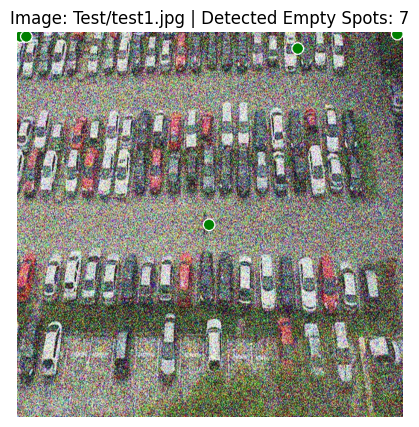
\includegraphics[width=\textwidth]{temp/sam1.png}
\caption{test1.jpg: 7 empty spots}
\label{fig:sam_test1}
\end{subfigure}
\hfill
\begin{subfigure}{0.48\textwidth}
\centering
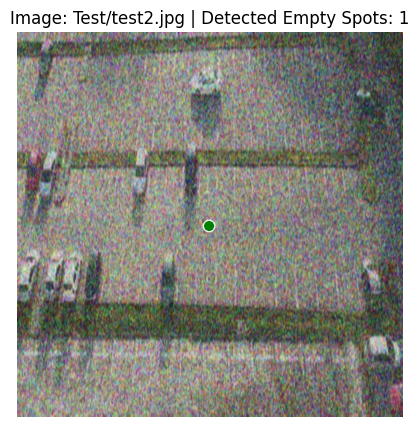
\includegraphics[width=\textwidth]{temp/sam2.png}
\caption{test2.jpg: 1 empty spot}
\label{fig:sam_test2}
\end{subfigure}
\vspace{0.5cm}
\begin{subfigure}{0.48\textwidth}
\centering
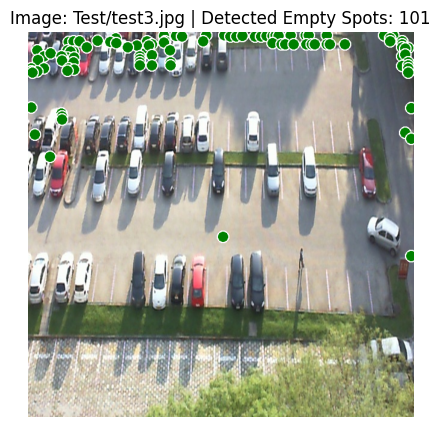
\includegraphics[width=\textwidth]{temp/sam3.png}
\caption{test3.jpg: 101 empty spots}
\label{fig:sam_test3}
\end{subfigure}
\hfill
\begin{subfigure}{0.48\textwidth}
\centering
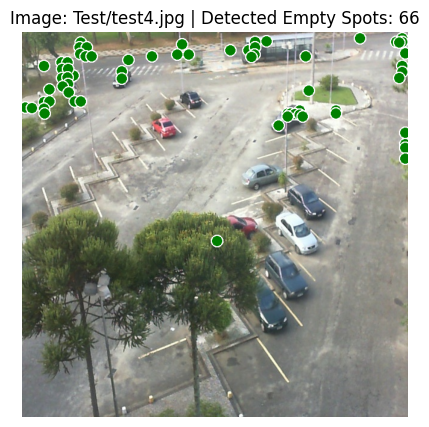
\includegraphics[width=\textwidth]{temp/sam4.png}
\caption{test4.jpg: 66 empty spots}
\label{fig:sam_test4}
\end{subfigure}
\vspace{0.5cm}
\begin{subfigure}{0.48\textwidth}
\centering
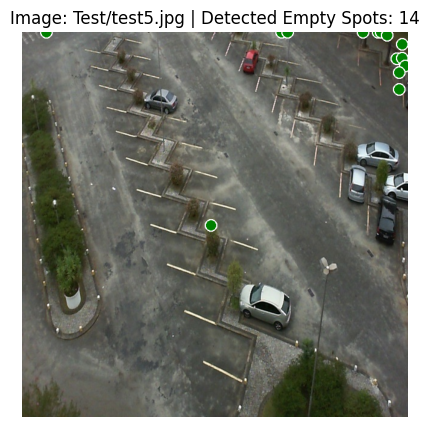
\includegraphics[width=\textwidth]{temp/sam5.png}
\caption{test5.jpg: 14 empty spots}
\label{fig:sam_test5}
\end{subfigure}
\hfill
\begin{subfigure}{0.48\textwidth}
\centering
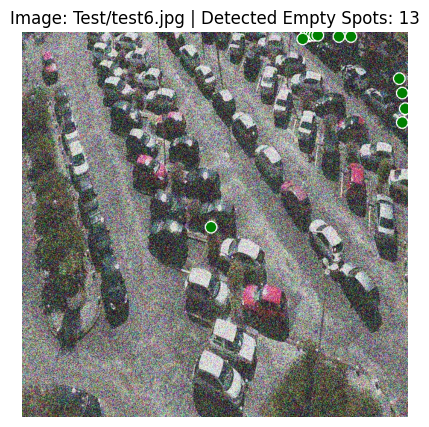
\includegraphics[width=\textwidth]{temp/sam6.png}
\caption{test6.jpg: 13 empty spots}
\label{fig:sam_test6}
\end{subfigure}
\caption{SAM Fine-Tuning Inference Results: Segmentation outputs on 6 test images showing detected empty parking spots. The model segments empty spaces using the two-stage fine-tuning approach.}
\label{fig:sam_inference}
\end{figure}

\textbf{Observations and Analysis:}

The inference conducted showed several important observations about the fine-tuned SAM model's performance:

\begin{itemize}
    \item \textbf{Inability to Identify Correct Locations:} The model demonstrated an inability to identify empty spots in the correct locations. The locations inferred were in the wrong spots, suggesting that the incomplete training (1.5 epochs in Stage 1, 300 batches in Stage 2) may not have been sufficient for the model to learn accurate spatial relationships.
    \item \textbf{Noise Sensitivity:} The model made fewer guesses with noise in the photo, indicating some robustness to image quality variations.
    \item \textbf{Edge Detection Bias:} In clear photos, the model made many guesses of empty spots along the edges of the image where there were many adjacent lines, tending to follow the linear curve of a road or lot. This suggests the model may be learning to detect linear features rather than actual parking space boundaries.
    \item \textbf{Training Completeness:} The obvious solution seems to be to complete training (5 + 5 epochs in 2 stages) to truly judge the potential of SAM to count empty spots. The current results represent an incomplete training process.
\end{itemize}

\textbf{Methodology Assessment:}

The attempted methodology would first (Stage 1) teach the model to segment parking spots, which it did not do before fine-tuning. Then Stage 2 would teach the model to segment just the empty parking spots, not those with cars in them. However, several challenges were encountered:

\begin{itemize}
    \item \textbf{Success Measurement:} The ability to measure success is not intuitive for this scenario. The SAM model on HuggingFace has its own measures for training (segmentation loss and IoU loss) that are not as relevant for the task of counting parking spots. IoU loss was ignored in this project and segmentation loss was considered, but the primary metric was Mean Absolute Error for counting accuracy.
    \item \textbf{Feasibility Question:} It is unclear whether this approach is feasible with HuggingFace SAM or would work better in a customized model that prioritizes counting specific objects (empty spots) from the onset of model building and training. The current implementation suggests that SAM may not be the optimal architecture for this specific counting task.
\end{itemize}

\textbf{Future Plans and Recommendations:}

\begin{enumerate}
    \item \textbf{Complete Training:} Require more time (ideally more computing power as well) to fully fine-tune SAM according to the planned methodology (5 + 5 epochs). Then require more time to adjust the process based on the results. The incomplete training prevents accurate assessment of the model's true potential.
    \item \textbf{Learning Rate Optimization:} Used 1e-5 for Stage 1 and 1e-6 for Stage 2, to lower the rate a little as the training progressed. This seemed ideal for batch size = 4, but with larger batch sizes such as 8 or 16, which require more computing power than laptop/desktop GPUs, the learning rates would have to increase with the batch sizes. For example, with linear scaling, LR would be 2e-5 for batch=8 and 4e-5 for batch=16.
    \item \textbf{Perturbation Method:} Perturbation was a method discovered in research but not attempted. It involves shifting bounding boxes around prior to training (bounding boxes identify the parking spots and formed the `masks' for segmentation loss). This could potentially improve model robustness and generalization.
    \item \textbf{Architecture Alternatives:} Consider whether a customized model architecture designed specifically for object counting tasks might be more suitable than adapting SAM for this purpose.
    \item \textbf{Evaluation Metrics:} Develop more appropriate evaluation metrics that better align with the counting task, potentially combining segmentation quality with counting accuracy.
\end{enumerate}

\section{Model Outputs on Sample Inputs}

This section presents visual examples of model predictions on sample parking lot images, demonstrating the detection capabilities of the trained models. The outputs show bounding boxes with class labels and confidence scores, providing insight into model performance on real-world scenarios.

\subsection{SSD Model Outputs}

Figure~\ref{fig:ssd_output} shows the SSD Lite model's predictions on a sample parking lot image. The model demonstrates good detection performance with bounding boxes color-coded by class: green for free parking spaces and red for occupied parking spaces. Each detection includes a confidence score, allowing assessment of the model's certainty in its predictions.

\begin{figure}[H]
\centering
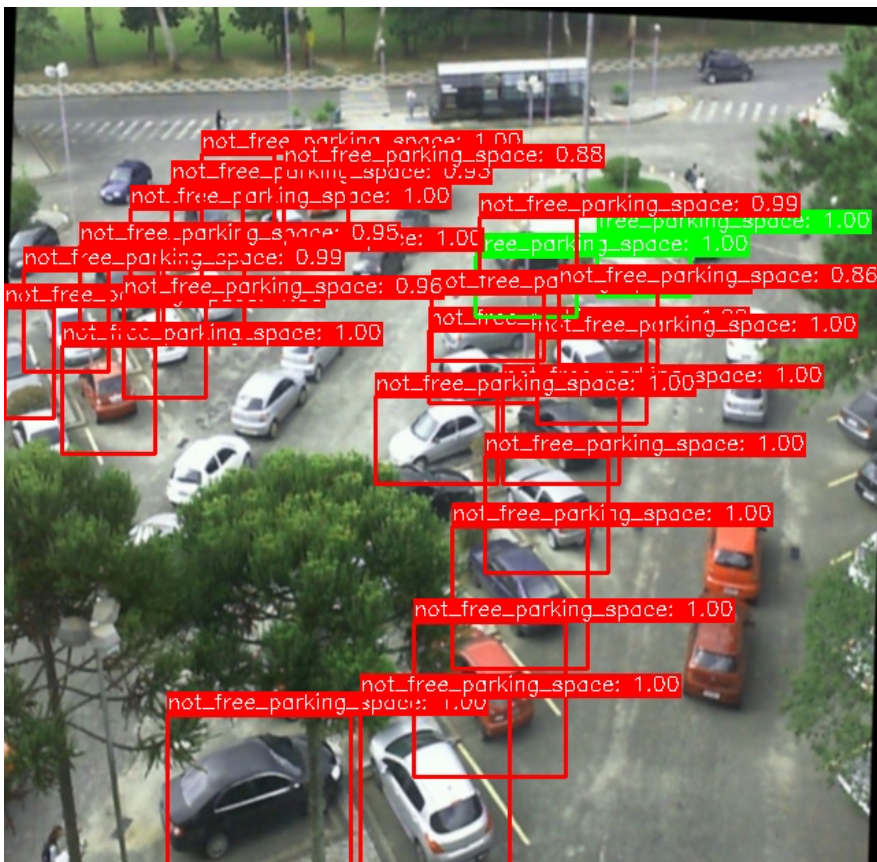
\includegraphics[width=0.95\textwidth]{temp/SSD - Output image .png}
\caption{SSD Model Output: Detection results on a sample parking lot image showing free parking spaces (green boxes) and occupied parking spaces (red boxes) with confidence scores. The SSD Lite model achieves 85.37\% mAP@50 and provides fast inference suitable for real-time applications.}
\label{fig:ssd_output}
\end{figure}

The SSD model successfully identifies multiple parking spaces with high confidence scores. The detections show accurate localization of both occupied and free spaces, demonstrating the model's ability to distinguish between different parking space states. The green bounding boxes indicate empty spaces that are available for parking, while red boxes mark spaces occupied by vehicles.

\subsection{Faster R-CNN Model Outputs}

Figure~\ref{fig:frcnn_output} demonstrates the Faster R-CNN model's predictions on the same parking lot scene. As the highest-performing model with 99.49\% mAP@50, Faster R-CNN shows superior detection accuracy with more precise bounding boxes and higher confidence scores compared to SSD.

\begin{figure}[H]
\centering
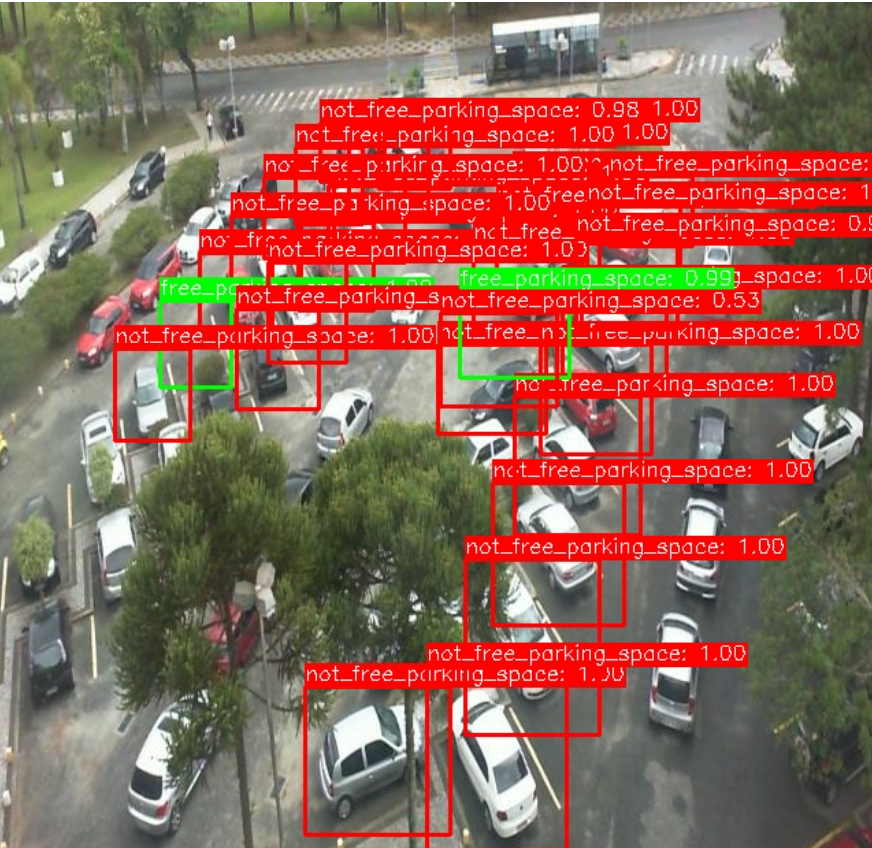
\includegraphics[width=0.95\textwidth]{temp/FRCNN - Output image .png}
\caption{Faster R-CNN Model Output: Detection results on a sample parking lot image showing free parking spaces (green boxes) and occupied parking spaces (red boxes) with confidence scores. The Faster R-CNN model achieves 99.49\% mAP@50, demonstrating the highest accuracy among all evaluated models.}
\label{fig:frcnn_output}
\end{figure}

The Faster R-CNN model demonstrates exceptional detection quality with very high confidence scores (predominantly 1.00 for both free and occupied spaces). The bounding boxes are precisely aligned with parking spaces and vehicles, showing minimal false positives or missed detections. This superior performance comes at the cost of slower inference speed compared to single-stage detectors, making it ideal for accuracy-critical applications where speed is less of a concern.

\subsection{Model Comparison on Sample Images}

Comparing the outputs from SSD and Faster R-CNN on the same parking lot scene reveals several key observations:

\begin{itemize}
    \item \textbf{Detection Accuracy:} Faster R-CNN shows more consistent high-confidence detections (predominantly 1.00) compared to SSD, which aligns with its superior mAP@50 performance (99.49\% vs. 85.37\%)
    \item \textbf{Bounding Box Precision:} Faster R-CNN's two-stage architecture produces more precise bounding boxes that closely align with parking space boundaries
    \item \textbf{False Positives:} Both models show minimal false positives, with Faster R-CNN demonstrating slightly better precision
    \item \textbf{Coverage:} Both models successfully detect the majority of visible parking spaces, with Faster R-CNN potentially identifying additional spaces that SSD may miss
    \item \textbf{Class Distinction:} Both models effectively distinguish between free (green) and occupied (red) parking spaces with high confidence
\end{itemize}

These visual outputs demonstrate the practical performance of the trained models and validate the quantitative metrics reported in the evaluation sections. The models successfully handle real-world parking lot scenarios with varying lighting conditions, vehicle types, and parking space configurations.

\subsection{SAM Model Outputs}

In addition to the object detection models, the fine-tuned SAM model provides segmentation-based outputs for parking space detection. As documented in Section~\ref{app:model_details}, SAM was tested on 6 sample images, detecting a total of 202 empty parking spots across the test set. The SAM outputs are visualized in Figures~\ref{fig:sam_test1} through~\ref{fig:sam_test6} in the Model Details appendix.

\section{Model Deployment}

This section describes the deployment infrastructure developed for the parking vision models, enabling real-world usage of the trained detection models through web-based interfaces and API endpoints.

\subsection{Deployment Architecture}

The deployment system consists of two main components: a Streamlit web application for interactive use and a FastAPI backend for programmatic access. The deployment supports local model deployment for SSD and Faster R-CNN models, providing flexible options for different use cases.

\textbf{Deployed Models:}
\begin{itemize}
    \item \textbf{SSD Lite 320 MobileNetV3:} Fast detection with good accuracy (85.37\% mAP@50), suitable for real-time applications
    \item \textbf{Faster R-CNN ResNet50 FPN:} Highest accuracy (99.49\% mAP@50), ideal for accuracy-critical applications
\end{itemize}

\subsection{Streamlit Web Application}

The primary deployment interface is a Streamlit web application that provides an intuitive, user-friendly interface for parking space detection. Figure~\ref{fig:deployment_landing} shows the landing page of the application with its clean, modern interface.

\begin{figure}[H]
\centering
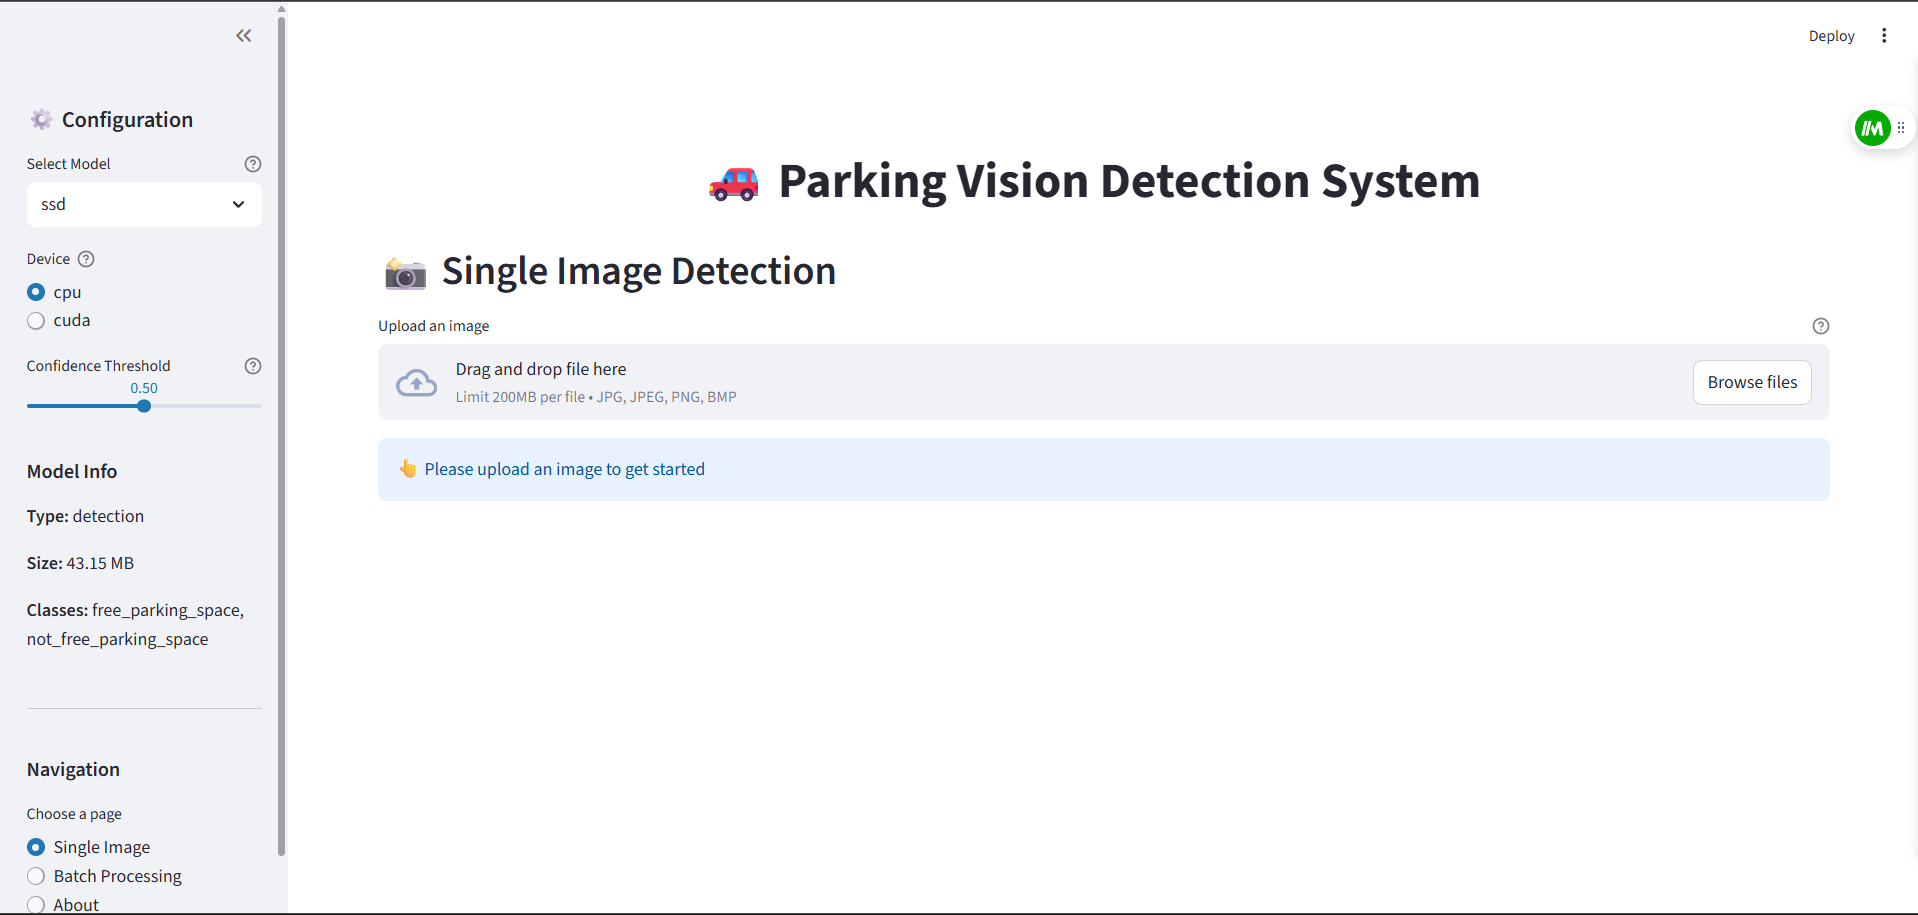
\includegraphics[width=0.9\textwidth]{temp/Deployment Images/Deployment Landing page .png}
\caption{Streamlit Web Application Landing Page: The main interface of the Parking Vision Detection System showing the welcome screen and application layout.}
\label{fig:deployment_landing}
\end{figure}

The application features a comprehensive set of capabilities:

\begin{itemize}
    \item \textbf{Model Selection:} Users can select between SSD and Faster R-CNN models from a sidebar interface, with automatic model availability detection
    \item \textbf{Device Selection:} Option to choose between CPU and GPU (CUDA) for inference, with automatic detection of available hardware
    \item \textbf{Confidence Threshold Control:} Adjustable confidence threshold slider (default: 0.5) to filter detections based on model certainty
    \item \textbf{Image Upload:} Support for uploading parking lot images through a drag-and-drop interface or file browser
    \item \textbf{Real-Time Visualization:} Automatic visualization of detection results with bounding boxes color-coded by class (green for free spaces, red for occupied spaces)
    \item \textbf{Detection Statistics:} Display of detection counts, confidence scores, and model performance metrics including free and occupied space counts
    \item \textbf{Results Export:} Ability to download detection results as JSON files for further analysis or integration with other systems
    \item \textbf{Model Caching:} Intelligent model caching using Streamlit's \texttt{@st.cache\_resource} decorator to avoid repeated loading and improve performance
    \item \textbf{Error Handling:} Comprehensive error handling with user-friendly error messages and troubleshooting guidance
\end{itemize}

The Streamlit application is launched using a simple batch script (\texttt{run.bat}) that automatically handles virtual environment activation, dependency checking (including automatic Streamlit installation if missing), and application startup. This makes deployment accessible to non-technical users who can simply double-click the batch file to start the application. The application runs on \texttt{http://localhost:8501} by default and opens automatically in the user's default web browser.

\textbf{SSD Model Interface:}
Figure~\ref{fig:deployment_ssd1} and Figure~\ref{fig:deployment_ssd2} show the Streamlit interface when using the SSD model. The interface displays the uploaded image with detection results, showing bounding boxes for detected parking spaces with color coding (green for free, red for occupied). The sidebar shows model selection, device options, and confidence threshold controls.

\begin{figure}[H]
\centering
\begin{subfigure}{0.48\textwidth}
\centering
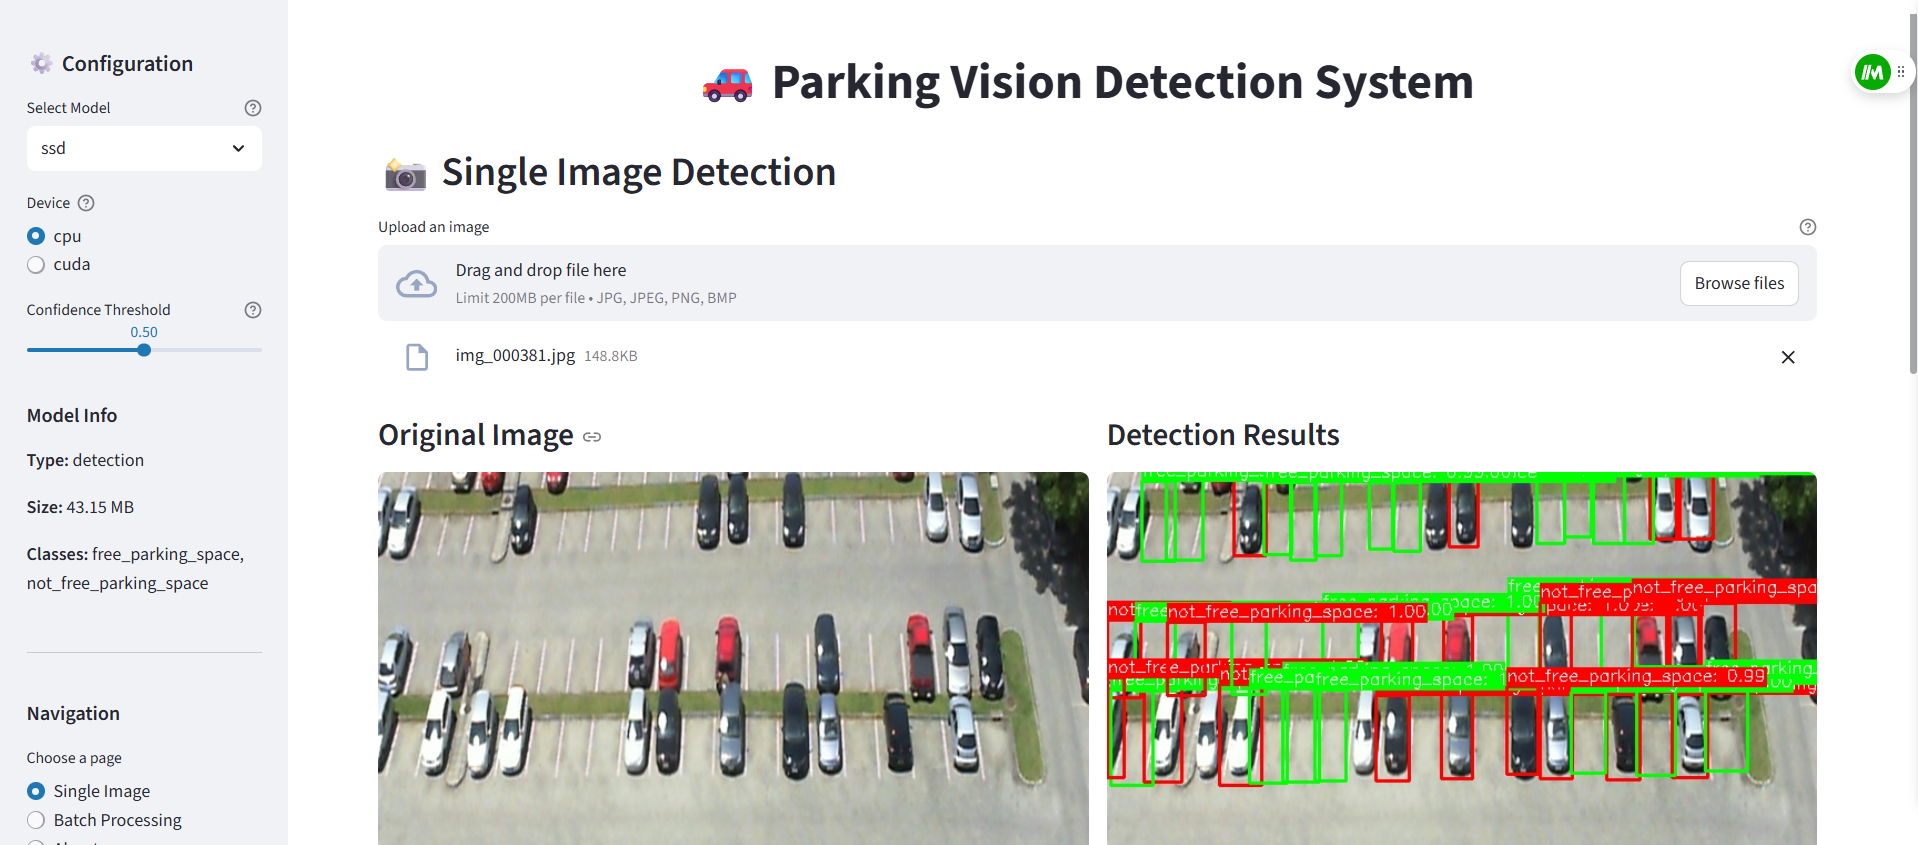
\includegraphics[width=\textwidth]{temp/Deployment Images/Deployment - SSD - 1.png}
\caption{SSD Model Interface - View 1}
\label{fig:deployment_ssd1}
\end{subfigure}
\hfill
\begin{subfigure}{0.48\textwidth}
\centering
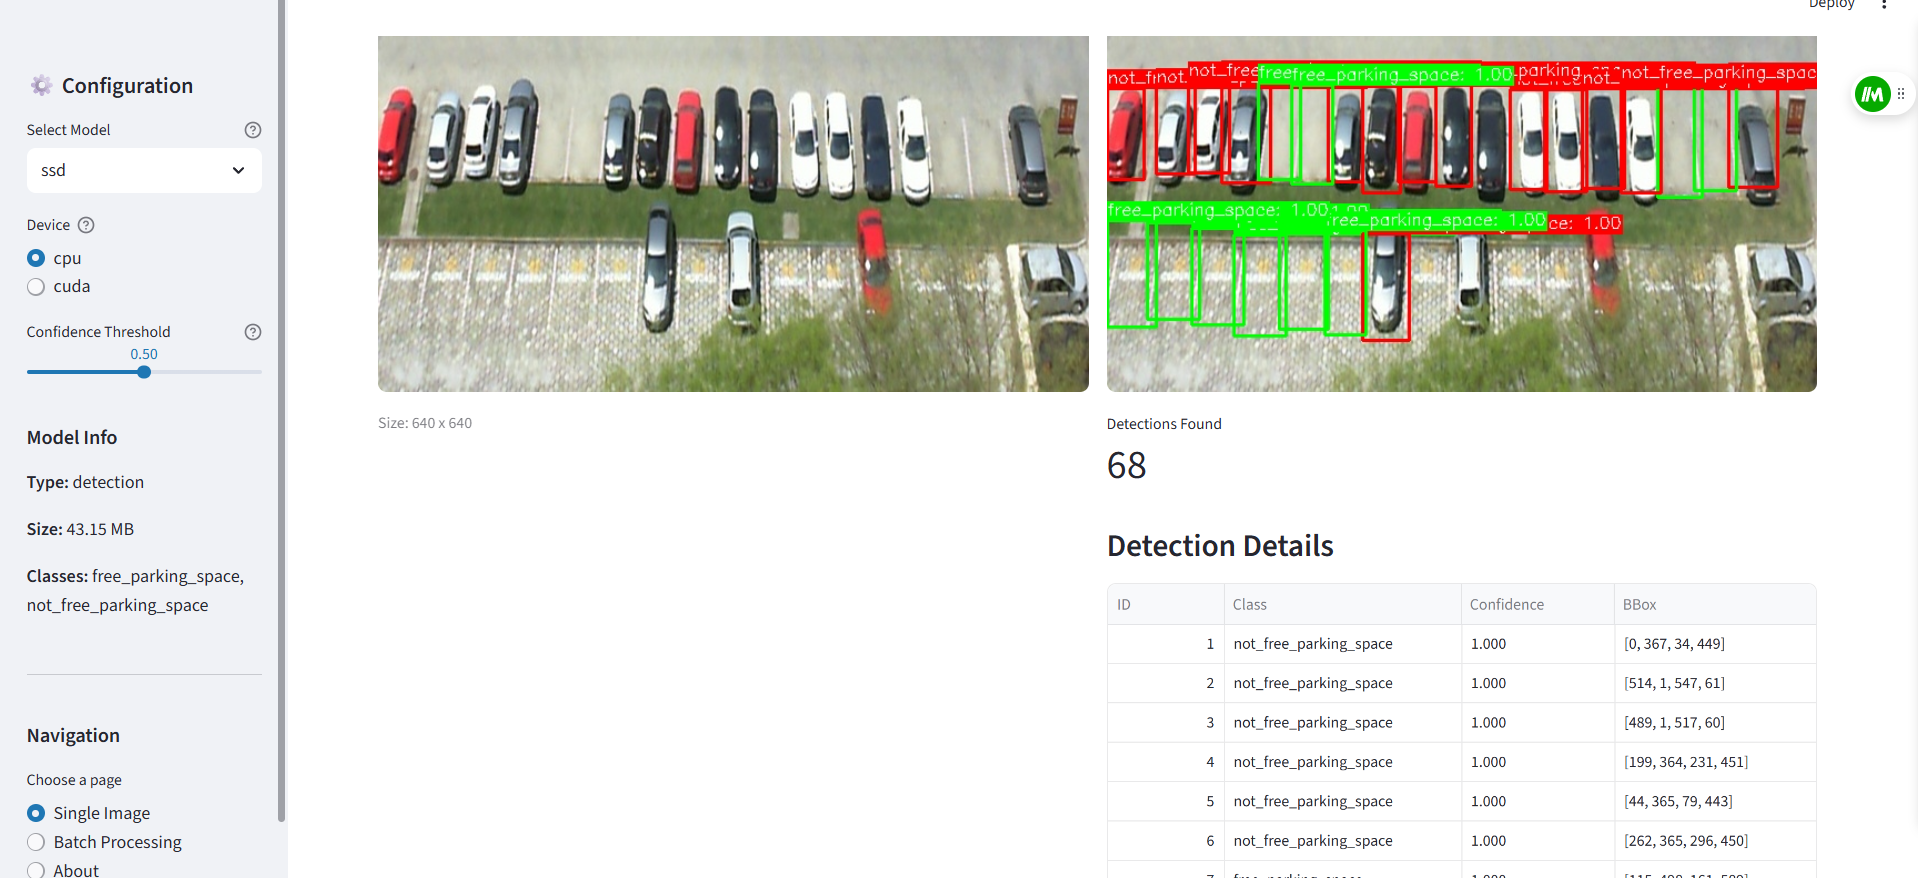
\includegraphics[width=\textwidth]{temp/Deployment Images/Deployment - SSD - 1.2.png}
\caption{SSD Model Interface - View 2}
\label{fig:deployment_ssd2}
\end{subfigure}
\caption{SSD Model Deployment Interface: The Streamlit web application showing SSD model inference results with detection visualizations, model configuration options, and detection statistics.}
\label{fig:deployment_ssd}
\end{figure}

\textbf{Faster R-CNN Model Interface:}
Figure~\ref{fig:deployment_frcnn1} and Figure~\ref{fig:deployment_frcnn2} demonstrate the interface when using the Faster R-CNN model. The higher accuracy of Faster R-CNN (99.49\% mAP@50) is reflected in more precise bounding boxes and higher confidence scores. The interface maintains the same user-friendly design while showcasing the superior detection quality of the two-stage detector.

\begin{figure}[H]
\centering
\begin{subfigure}{0.48\textwidth}
\centering
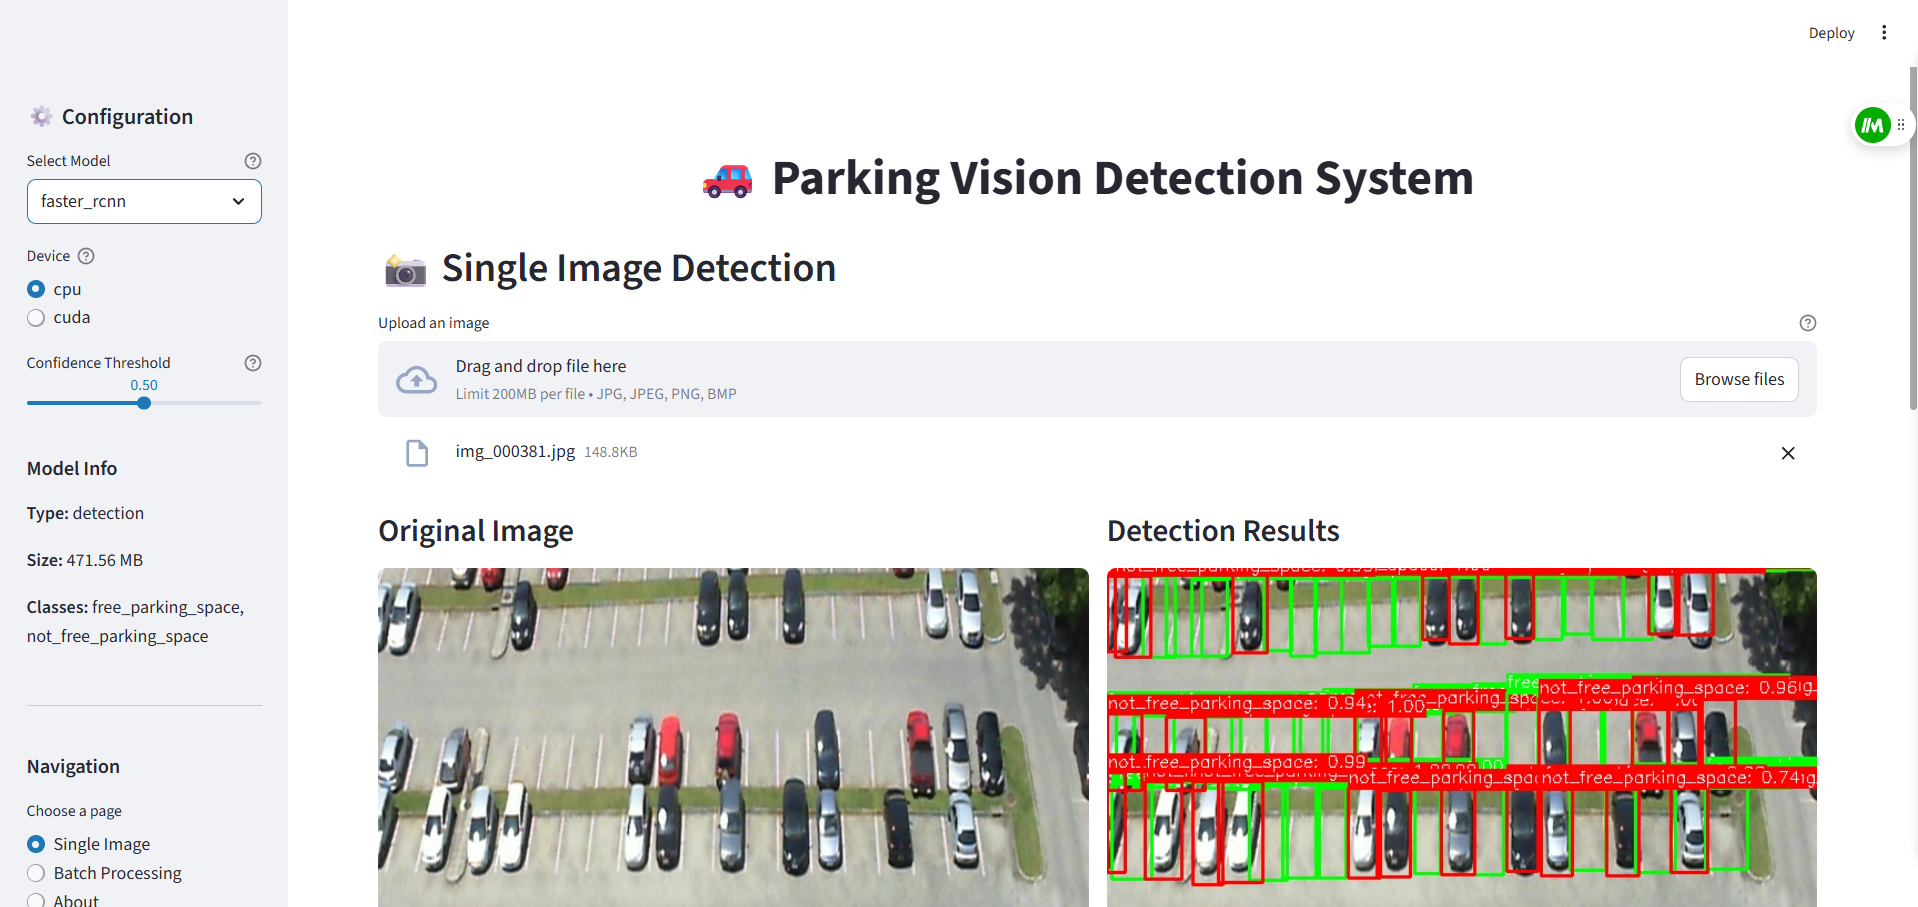
\includegraphics[width=\textwidth]{temp/Deployment Images/Deployment - FRCNN - 1.png}
\caption{Faster R-CNN Model Interface - View 1}
\label{fig:deployment_frcnn1}
\end{subfigure}
\hfill
\begin{subfigure}{0.48\textwidth}
\centering
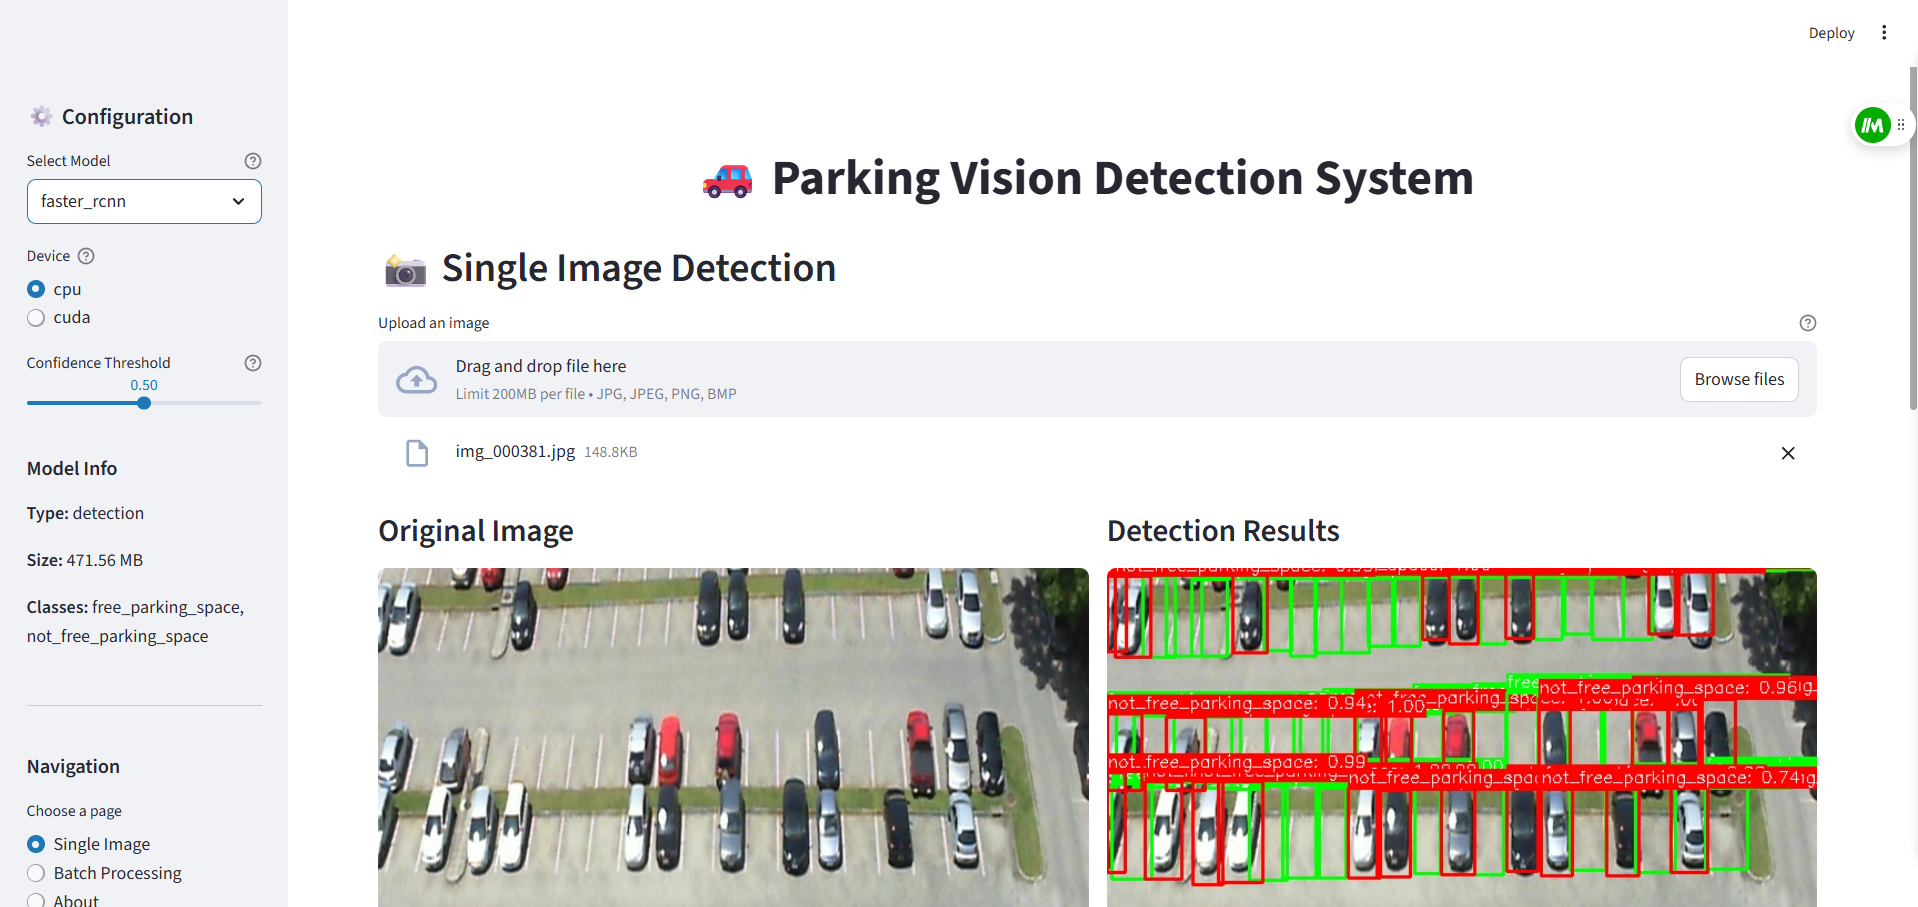
\includegraphics[width=\textwidth]{temp/Deployment Images/Deployment - FRCNN - 1.2.png}
\caption{Faster R-CNN Model Interface - View 2}
\label{fig:deployment_frcnn2}
\end{subfigure}
\caption{Faster R-CNN Model Deployment Interface: The Streamlit web application showing Faster R-CNN model inference results with high-accuracy detections, detailed statistics, and visualization of parking space occupancy.}
\label{fig:deployment_frcnn}
\end{figure}

\subsection{FastAPI Backend}

For programmatic access and integration with other systems, a FastAPI backend provides RESTful API endpoints:

\begin{itemize}
    \item \textbf{Health Check:} \texttt{/health} endpoint for system status monitoring
    \item \textbf{Model Management:} \texttt{/models} endpoint to list available models and their status
    \item \textbf{Model Loading:} \texttt{/models/load} endpoint to dynamically load models into memory
    \item \textbf{Single Image Inference:} \texttt{/predict} endpoint for processing individual images
    \item \textbf{Batch Inference:} \texttt{/predict/batch} endpoint for processing multiple images simultaneously
    \item \textbf{Model Information:} \texttt{/models/\{model\_name\}} endpoint to retrieve detailed model specifications
\end{itemize}

The FastAPI backend includes CORS middleware for cross-origin requests, enabling integration with web applications and other services. The API returns structured JSON responses with detection results, confidence scores, and bounding box coordinates.

\subsection{Deployment Infrastructure}

\textbf{File Structure:}
The deployment system follows a modular architecture with clear separation of concerns:

\begin{itemize}
    \item \textbf{Model Checkpoints:} Trained models stored in \texttt{checkpoints/} directory with separate folders for each model type:
    \begin{itemize}
        \item \texttt{checkpoints/phase2\_ssd\_parking/best\_model.pt} - SSD model checkpoint
        \item \texttt{checkpoints/phase2\_faster\_rcnn\_parking/best\_model.pt} - Faster R-CNN model checkpoint
    \end{itemize}
    \item \textbf{Model Loading Utilities (\texttt{models/}):} 
    \begin{itemize}
        \item \texttt{model\_loader.py} - Unified interface for loading different model architectures
        \item \texttt{architectures.py} - Model architecture definitions and builders
    \end{itemize}
    \item \textbf{Inference Module (\texttt{inference/}):}
    \begin{itemize}
        \item \texttt{single\_inference.py} - Single image prediction functions
        \item \texttt{batch\_inference.py} - Batch processing capabilities
    \end{itemize}
    \item \textbf{Utilities (\texttt{utils/}):}
    \begin{itemize}
        \item \texttt{image\_utils.py} - Image loading, preprocessing, and format conversion
        \item \texttt{visualization.py} - Drawing bounding boxes and detection overlays
    \end{itemize}
    \item \textbf{Application Files:}
    \begin{itemize}
        \item \texttt{streamlit\_app.py} - Main Streamlit web application (307 lines)
        \item \texttt{app.py} - FastAPI backend API (222 lines)
        \item \texttt{predict\_image.py} - Command-line tool for single image inference
        \item \texttt{predict\_batch.py} - Command-line tool for batch processing
        \item \texttt{run.bat} - Windows batch script for easy startup
        \item \texttt{Dockerfile} - Container deployment configuration
    \end{itemize}
    \item \textbf{Configuration:}
    \begin{itemize}
        \item \texttt{requirements.txt} - Python dependencies (Streamlit, PyTorch, OpenCV, etc.)
        \item \texttt{.streamlit/} - Streamlit configuration directory
    \end{itemize}
\end{itemize}

\textbf{Model Loading System:}
The deployment uses a sophisticated model loading system that:
\begin{itemize}
    \item Automatically detects available model checkpoints
    \item Handles different model architectures (SSD, Faster R-CNN) with unified interface
    \item Supports both CPU and GPU inference based on hardware availability
    \item Implements model caching to avoid repeated loading
    \item Provides model information including architecture details and checkpoint paths
\end{itemize}

\textbf{Inference Capabilities:}
\begin{itemize}
    \item \textbf{Single Image Inference:} Process individual images with configurable confidence thresholds
    \item \textbf{Batch Inference:} Process multiple images efficiently with batch processing
    \item \textbf{Preprocessing:} Automatic image preprocessing including resizing, normalization, and format conversion
    \item \textbf{Post-processing:} Non-maximum suppression, confidence filtering, and result formatting
    \item \textbf{Visualization:} Automatic generation of annotated images with bounding boxes and labels
\end{itemize}

\subsection{Deployment Features}

\textbf{Ease of Use:}
\begin{itemize}
    \item One-click deployment via \texttt{run.bat} script
    \item Automatic dependency installation and virtual environment management
    \item User-friendly web interface requiring no technical knowledge
    \item Clear error messages and troubleshooting guidance
\end{itemize}

\textbf{Performance:}
\begin{itemize}
    \item Efficient model loading with caching to minimize startup time
    \item GPU acceleration support when available
    \item Optimized inference pipelines for both SSD and Faster R-CNN
    \item Batch processing capabilities for handling multiple images
\end{itemize}

\textbf{Extensibility:}
\begin{itemize}
    \item Modular architecture allowing easy addition of new models
    \item API-based design enabling integration with other systems
    \item Support for custom confidence thresholds and filtering options
    \item JSON export for integration with downstream analysis tools
\end{itemize}

\subsection{Command-Line Tools}

In addition to the web interface, the deployment includes command-line tools for programmatic access and batch processing:

\textbf{Single Image Prediction (\texttt{predict\_image.py}):}
\begin{itemize}
    \item Process individual images from the command line
    \item Supports both SSD and Faster R-CNN models
    \item Configurable confidence threshold and device selection
    \item Automatic output directory creation with visualization and JSON results
    \item Usage: \texttt{python predict\_image.py --model ssd --image path/to/image.jpg --output results/}
\end{itemize}

\textbf{Batch Processing (\texttt{predict\_batch.py}):}
\begin{itemize}
    \item Process multiple images in a directory
    \item Efficient batch inference for large datasets
    \item Generates individual results for each image
    \item Summary statistics across all processed images
    \item Usage: \texttt{python predict\_batch.py --model faster\_rcnn --input images/ --output results/}
\end{itemize}

\subsection{Docker Deployment}

The deployment system includes Docker support for containerized deployment. The \texttt{Dockerfile} provides:

\begin{itemize}
    \item \textbf{Base Image:} Python 3.10-slim for lightweight containers
    \item \textbf{System Dependencies:} OpenGL libraries, image processing libraries (libgl1-mesa-glx, libglib2.0-0, etc.)
    \item \textbf{Application Setup:} Automatic dependency installation from \texttt{requirements.txt}
    \item \textbf{Port Configuration:} Exposes port 8000 for FastAPI backend
    \item \textbf{Directory Structure:} Creates necessary directories (\texttt{static/uploads/}) for file handling
    \item \textbf{Startup Command:} Uses uvicorn to run the FastAPI application
\end{itemize}

Docker deployment enables consistent deployment across different environments and simplifies production deployment.

\subsection{Usage Workflow}

\textbf{Web Interface Workflow:}
The typical deployment workflow using the Streamlit web interface is as follows:

\begin{enumerate}
    \item \textbf{Startup:} User runs \texttt{run.bat} which:
    \begin{itemize}
        \item Activates the virtual environment (checks for existence)
        \item Verifies Streamlit installation (installs if missing)
        \item Starts the Streamlit application on \texttt{http://localhost:8501}
        \item Opens the application in the default web browser
    \end{itemize}
    \item \textbf{Page Selection:} User selects between "Single Image", "Batch Processing", or "About" pages
    \item \textbf{Model Selection:} User selects desired model (SSD or Faster R-CNN) from the sidebar
    \item \textbf{Device Selection:} User chooses CPU or CUDA (GPU) for inference
    \item \textbf{Configuration:} User adjusts confidence threshold if needed (default: 0.5, range: 0.0-1.0)
    \item \textbf{Image Upload:} User uploads a parking lot image (JPG, JPEG, PNG, BMP formats supported)
    \item \textbf{Processing:} System:
    \begin{itemize}
        \item Loads the model (cached after first load using \texttt{@st.cache\_resource})
        \item Preprocesses the image (converts to RGB, handles format conversion)
        \item Runs inference with the selected model and confidence threshold
        \item Post-processes results (non-maximum suppression, filtering)
    \end{itemize}
    \item \textbf{Visualization:} Results are displayed with:
    \begin{itemize}
        \item Annotated image with bounding boxes (green for free, red for occupied)
        \item Detection count metric
        \item Detailed detection table with ID, class, confidence, and bounding box coordinates
    \end{itemize}
    \item \textbf{Export:} User can download results as JSON file containing all detection details
\end{enumerate}

\textbf{API Workflow:}
For programmatic access via FastAPI:

\begin{enumerate}
    \item \textbf{Health Check:} Verify system status with \texttt{GET /health}
    \item \textbf{List Models:} Get available models with \texttt{GET /models}
    \item \textbf{Load Model:} Load model into memory with \texttt{POST /models/load}
    \item \textbf{Predict:} Send image and receive JSON response with \texttt{POST /predict}
    \item \textbf{Batch Predict:} Process multiple images with \texttt{POST /predict/batch}
\end{enumerate}

\subsection{Technical Implementation Details}

The deployment system handles several technical challenges:

\begin{itemize}
    \item \textbf{Model Architecture Differences:} Unified interface for different model architectures (SSD vs. Faster R-CNN) with architecture-specific handling
    \item \textbf{Device Management:} Automatic detection and utilization of GPU when available, with fallback to CPU
    \item \textbf{Memory Management:} Efficient model loading and caching to minimize memory usage
    \item \textbf{Image Format Handling:} Support for various image formats (JPEG, PNG) with automatic conversion
    \item \textbf{Error Handling:} Comprehensive error handling for missing models, invalid images, and inference failures
    \item \textbf{Dependency Management:} Automatic checking and installation of required packages (Streamlit, transformers)
\end{itemize}

\subsection{Technical Implementation Details}

The deployment system handles several technical challenges:

\begin{itemize}
    \item \textbf{Model Architecture Differences:} Unified interface for different model architectures (SSD vs. Faster R-CNN) with architecture-specific handling through \texttt{models/architectures.py}
    \item \textbf{Device Management:} Automatic detection and utilization of GPU when available, with fallback to CPU. Device selection is configurable in both web interface and API
    \item \textbf{Memory Management:} Efficient model loading and caching using Streamlit's \texttt{@st.cache\_resource} decorator to minimize memory usage and avoid repeated loading
    \item \textbf{Image Format Handling:} Support for various image formats (JPEG, PNG, BMP) with automatic conversion to RGB format required by PyTorch models
    \item \textbf{Temporary File Management:} Secure handling of uploaded images using temporary files with unique timestamps, automatic cleanup after processing
    \item \textbf{Error Handling:} Comprehensive error handling for:
    \begin{itemize}
        \item Missing models or checkpoints
        \item Invalid image formats
        \item Inference failures
        \item Model loading errors
        \item Device availability issues
    \end{itemize}
    \item \textbf{Dependency Management:} Automatic checking and installation of required packages (Streamlit, transformers) with clear error messages if installation fails
    \item \textbf{Cross-Platform Support:} Batch scripts for Windows, with Docker support for Linux and containerized deployments
\end{itemize}

\subsection{Deployment Status}

The deployment system has been successfully implemented and tested for:

\begin{itemize}
    \item \textbf{Local Deployment:} Successfully deployed on Windows systems with one-click startup via \texttt{run.bat}
    \item \textbf{SSD Model:} Real-time inference performance with 85.37\% mAP@50 accuracy, suitable for interactive use
    \item \textbf{Faster R-CNN Model:} High-accuracy inference with 99.49\% mAP@50, demonstrating superior detection quality
    \item \textbf{Web Interface:} Fully functional Streamlit application with intuitive user interface, model selection, and real-time visualization
    \item \textbf{API Endpoints:} Complete FastAPI backend with RESTful endpoints for programmatic access
    \item \textbf{Batch Processing:} Command-line tools for processing multiple images efficiently
    \item \textbf{Docker Support:} Containerized deployment ready for production environments
    \item \textbf{Model Caching:} Efficient model loading with caching to minimize startup time and memory usage
    \item \textbf{GPU Support:} CUDA acceleration when GPU hardware is available
\end{itemize}

This deployment infrastructure provides a production-ready system for utilizing the trained parking vision models in real-world scenarios. The combination of user-friendly web interface, programmatic API access, and command-line tools makes the research results accessible and practical for both technical and non-technical end users. The modular architecture ensures easy extensibility for adding new models or features in the future.

\section{Agile Development Methodology}

This section documents the agile development methodology used throughout the Parking Vision project. The project followed Scrum framework principles with three sprints over a three-week period, enabling rapid development and iterative improvement of the parking space detection system.

\subsection{Methodology Overview}

\textbf{Framework:} Scrum  
\textbf{Sprint Duration:} 1 week per sprint  
\textbf{Total Sprints:} 3 sprints  
\textbf{Team Size:} 5 members  
\textbf{Total Story Points:} 118 SP  
\textbf{Project Duration:} November 16 - December 7, 2025

The project was organized into four main epics:
\begin{enumerate}
    \item \textbf{Phase 1: Baseline Models and Dataset Exploration} (13 SP)
    \item \textbf{Phase 1.5: SAM Fine-tuning and Data Processing} (18 SP)
    \item \textbf{Phase 2: Advanced Model Training and Optimization} (34 SP)
    \item \textbf{Deployment and API Development} (13 SP)
\end{enumerate}

\subsection{Sprint Planning and Execution}

\subsubsection{Sprint 1: Project Setup and Idea Finalization (Nov 16-23, 2025)}

\textbf{Sprint Goal:} Finalize project idea and establish project foundation

\textbf{Sprint Backlog (13 Story Points):}
\begin{itemize}
    \item Project Setup and Idea Finalization (3 SP)
    \item Dataset Exploration and Analysis (5 SP)
    \item CNN Baseline Model Implementation (5 SP)
\end{itemize}

\textbf{Key Deliverables:}
\begin{itemize}
    \item Project idea finalized (Parking Lot Detection)
    \item Development environment configured
    \item Dataset exploration completed with comprehensive EDA
    \item CNN baseline model trained and evaluated (96\% accuracy)
\end{itemize}

\textbf{Team Assignments:}
\begin{itemize}
    \item Francis Cho: Project setup and idea finalization
    \item Sugakabiyrarosha: Dataset exploration, CNN baseline development
\end{itemize}

\subsubsection{Sprint 2: Phase 1 \& Phase 1.5 Implementation (Nov 23-30, 2025)}

\textbf{Sprint Goal:} Implement Phase 1 object detection models and Phase 1.5 SAM fine-tuning

\textbf{Sprint Backlog (55 Story Points):}

\textbf{Phase 1 (37 SP):}
\begin{itemize}
    \item SSD Model Training (8 SP)
    \item Faster R-CNN Model Training (8 SP)
    \item DETR Model Training (8 SP)
    \item YOLO Model Training (8 SP)
    \item Model Comparison and Evaluation (5 SP)
\end{itemize}

\textbf{Phase 1.5 (18 SP):}
\begin{itemize}
    \item SAM Model Fine-tuning (8 SP)
    \item Image Alignment and Template Matching (5 SP)
    \item Training Data Clustering (5 SP)
\end{itemize}

\textbf{Key Deliverables:}
\begin{itemize}
    \item Four object detection models trained (SSD, Faster R-CNN, DETR, YOLO)
    \item SAM model fine-tuned for parking segmentation
    \item Image alignment pipeline implemented
    \item Data clustering analysis completed
    \item Comprehensive model comparison report
\end{itemize}

\textbf{Team Assignments:}
\begin{itemize}
    \item Sugakabiyrarosha: SSD, DETR model training, image alignment
    \item Alvis Chi Hin Ngan: Faster R-CNN implementation and training
    \item Hitakshi Chugh: YOLO implementation and training
    \item Francis Cho: SAM fine-tuning, model comparison
    \item John Allan Ellingson: Clustering pipeline, visualizations
\end{itemize}

\subsubsection{Sprint 3: Phase 2, Deployment \& Report (Dec 1-7, 2025)}

\textbf{Sprint Goal:} Complete Phase 2 model optimization, deploy API, and finalize report

\textbf{Sprint Backlog (50 Story Points):}

\textbf{Phase 2 (34 SP):}
\begin{itemize}
    \item Data Augmentation Pipeline (8 SP)
    \item Augmented Dataset EDA (5 SP)
    \item SSD Phase 2 Training with Hyperparameter Tuning (8 SP)
    \item Faster R-CNN Phase 2 Training with Optimization (8 SP)
    \item DETR Phase 2 Training (8 SP)
    \item YOLO Phase 2 Training (8 SP)
    \item CNN Patch Classifier Implementation (5 SP)
    \item Phase 2 Model Comparison (5 SP)
\end{itemize}

\textbf{Deployment (13 SP):}
\begin{itemize}
    \item API Development - FastAPI Backend (8 SP)
    \item Model Loader and Architecture Abstraction (5 SP)
    \item Inference Pipeline Implementation (5 SP)
    \item Docker Containerization (3 SP)
    \item Deployment Documentation (2 SP)
\end{itemize}

\textbf{Report (8 SP):}
\begin{itemize}
    \item Main Report Writing (8 SP)
    \item Report Writing Assistance (5 SP)
\end{itemize}

\textbf{Key Deliverables:}
\begin{itemize}
    \item Comprehensive data augmentation pipeline (36,426 images)
    \item All models retrained with optimized hyperparameters
    \item CNN patch classifier implemented
    \item Phase 2 model comparison completed
    \item FastAPI backend with all endpoints
    \item Unified model loading system
    \item Single and batch inference pipelines
    \item Docker containerization
    \item Comprehensive deployment documentation
    \item Complete project report
\end{itemize}

\textbf{Team Assignments:}
\begin{itemize}
    \item Sugakabiyrarosha: SSD/DETR Phase 2 training, hyperparameter tuning, API development, model deployment, main report writing
    \item Alvis Chi Hin Ngan: Data augmentation, Faster R-CNN Phase 2 optimization, GPU assistance
    \item Hitakshi Chugh: YOLO Phase 2 training, model comparison
    \item Francis Cho: Model comparison, results analysis, report assistance
    \item John Allan Ellingson: Augmented dataset EDA, visualizations, statistical analyses, report assistance
\end{itemize}

\subsection{Project Metrics and Velocity}

\textbf{Velocity Tracking:}
\begin{itemize}
    \item Sprint 1: 13 SP completed
    \item Sprint 2: 55 SP completed
    \item Sprint 3: 50 SP completed
    \item \textbf{Total: 118 Story Points}
    \item \textbf{Average Velocity:} 39.3 SP per sprint
    \item \textbf{Completion Rate:} 100\% (118/118 SP)
\end{itemize}

Figure~\ref{fig:velocity_chart} shows the team's velocity across all sprints, demonstrating consistent high performance throughout the project.

\begin{figure}[H]
\centering
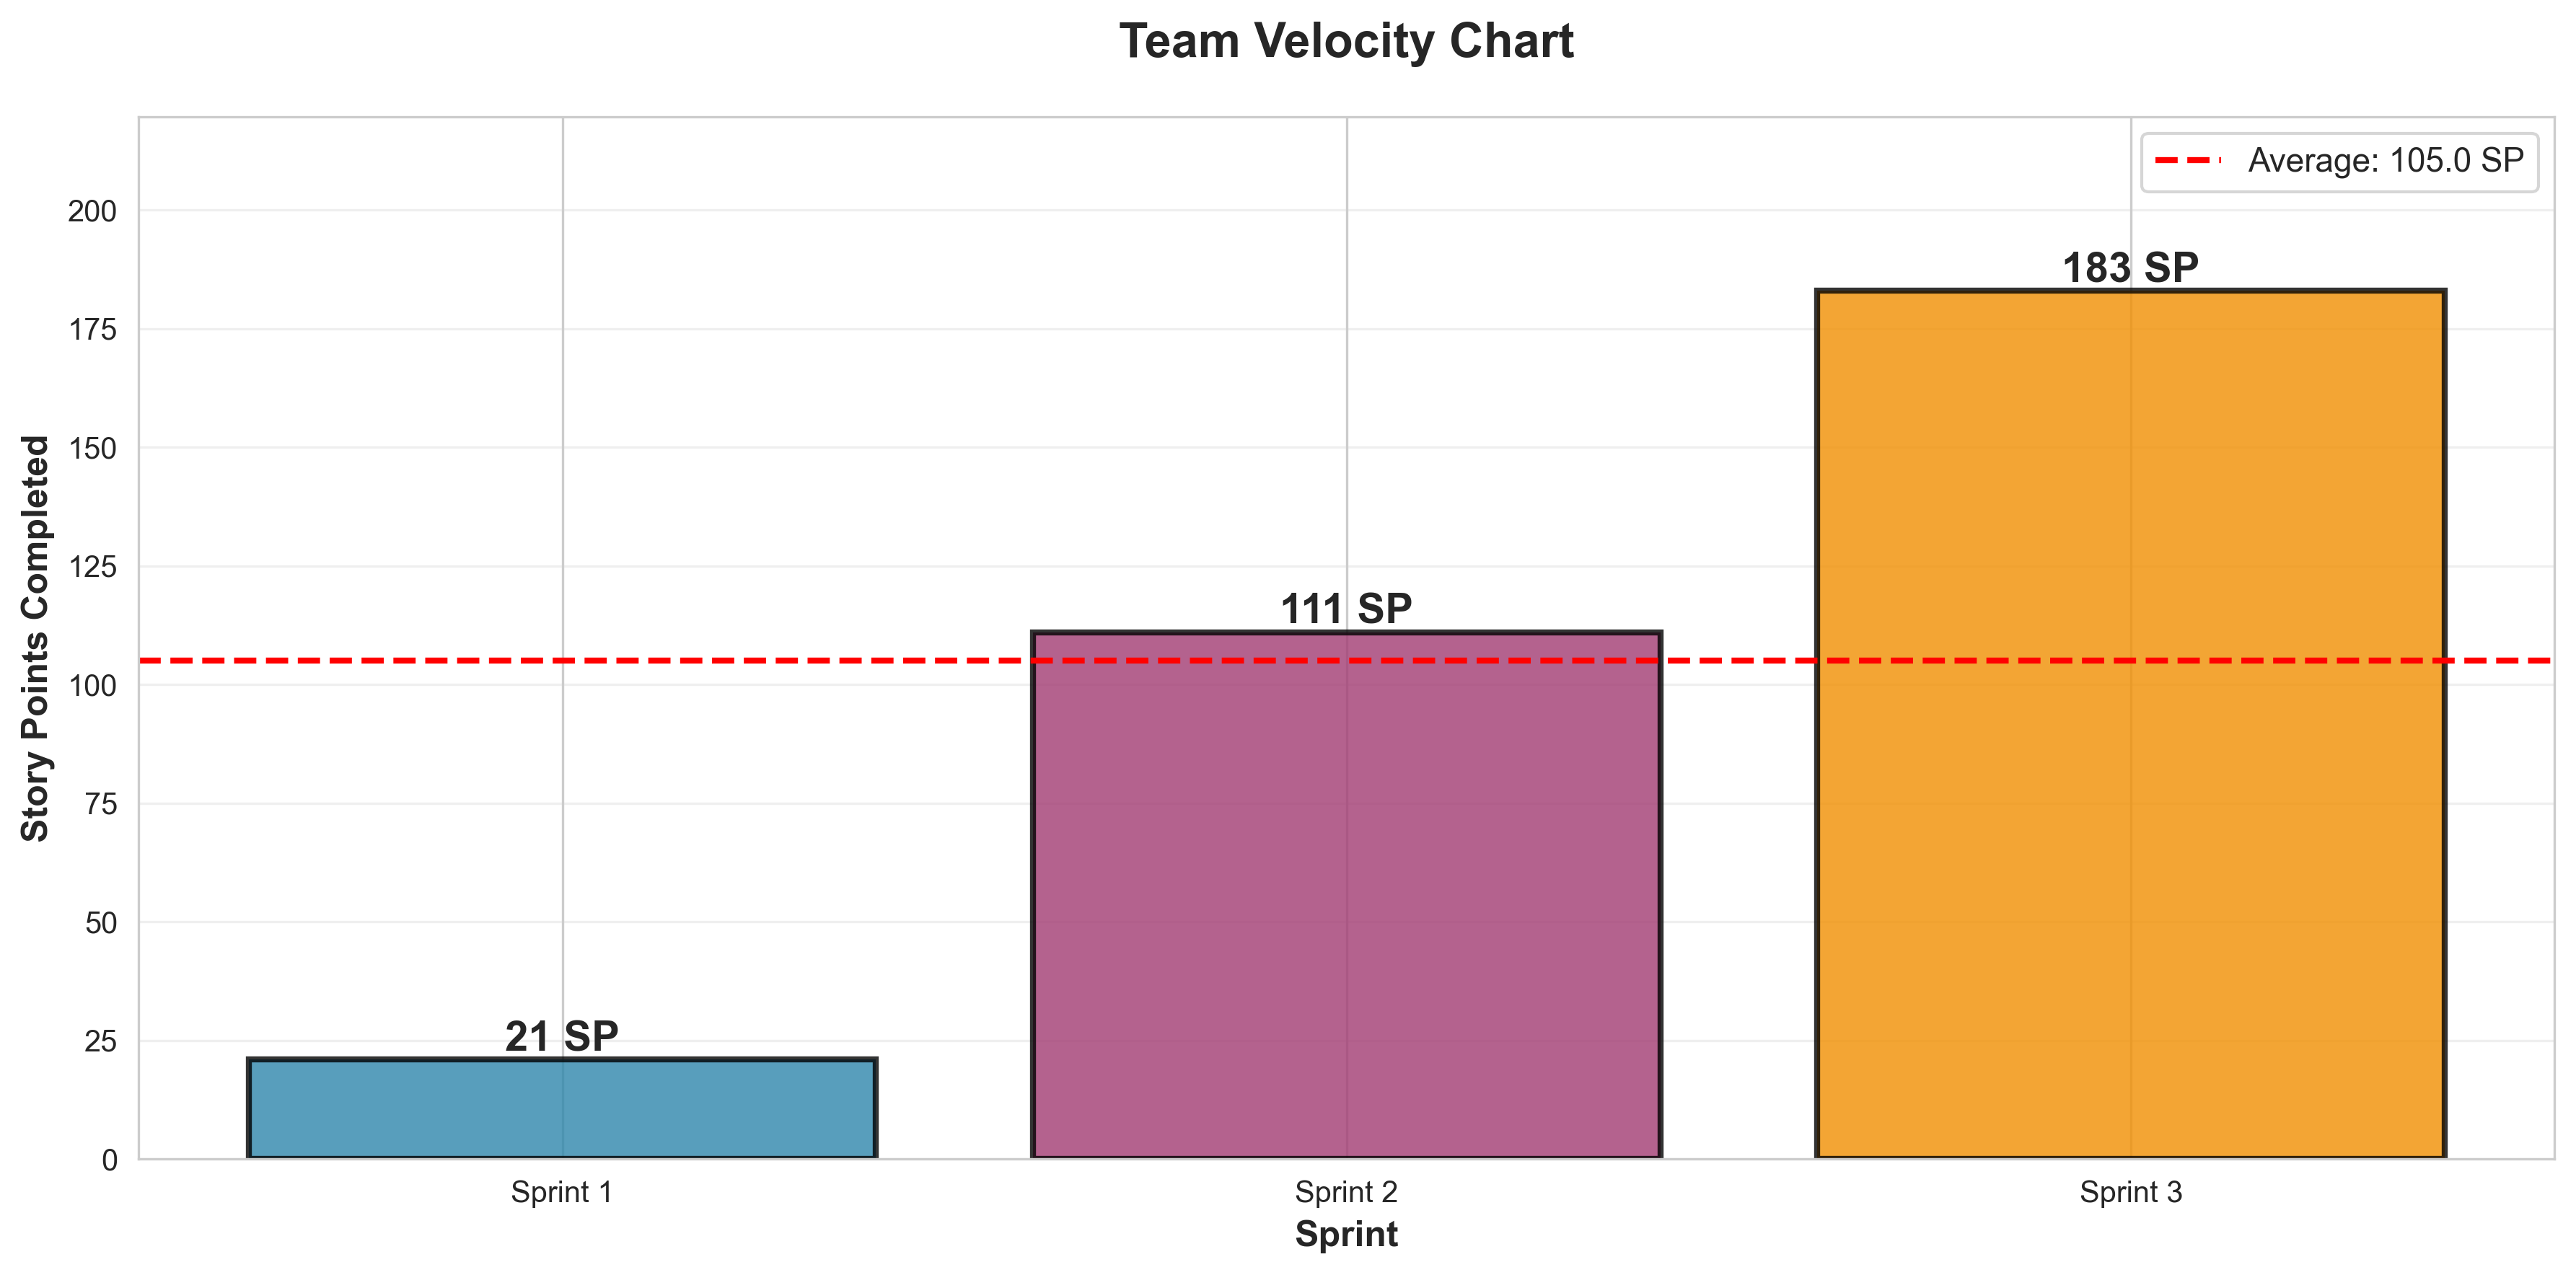
\includegraphics[width=0.8\textwidth]{temp/velocity_chart.png}
\caption{Team Velocity Chart: Story points completed per sprint showing consistent high performance across all three sprints.}
\label{fig:velocity_chart}
\end{figure}

\subsection{Burndown Charts}

Burndown charts track the progress of work completion throughout each sprint and the overall project. These charts show the remaining story points over time, helping identify if the team is on track to complete all planned work.

\textbf{Sprint 1 Burndown (Nov 16-23, 2025):}
Figure~\ref{fig:burndown_sprint1} shows the burndown for Sprint 1, which focused on project setup and baseline establishment. The team completed all 13 story points as planned.

\begin{figure}[H]
\centering
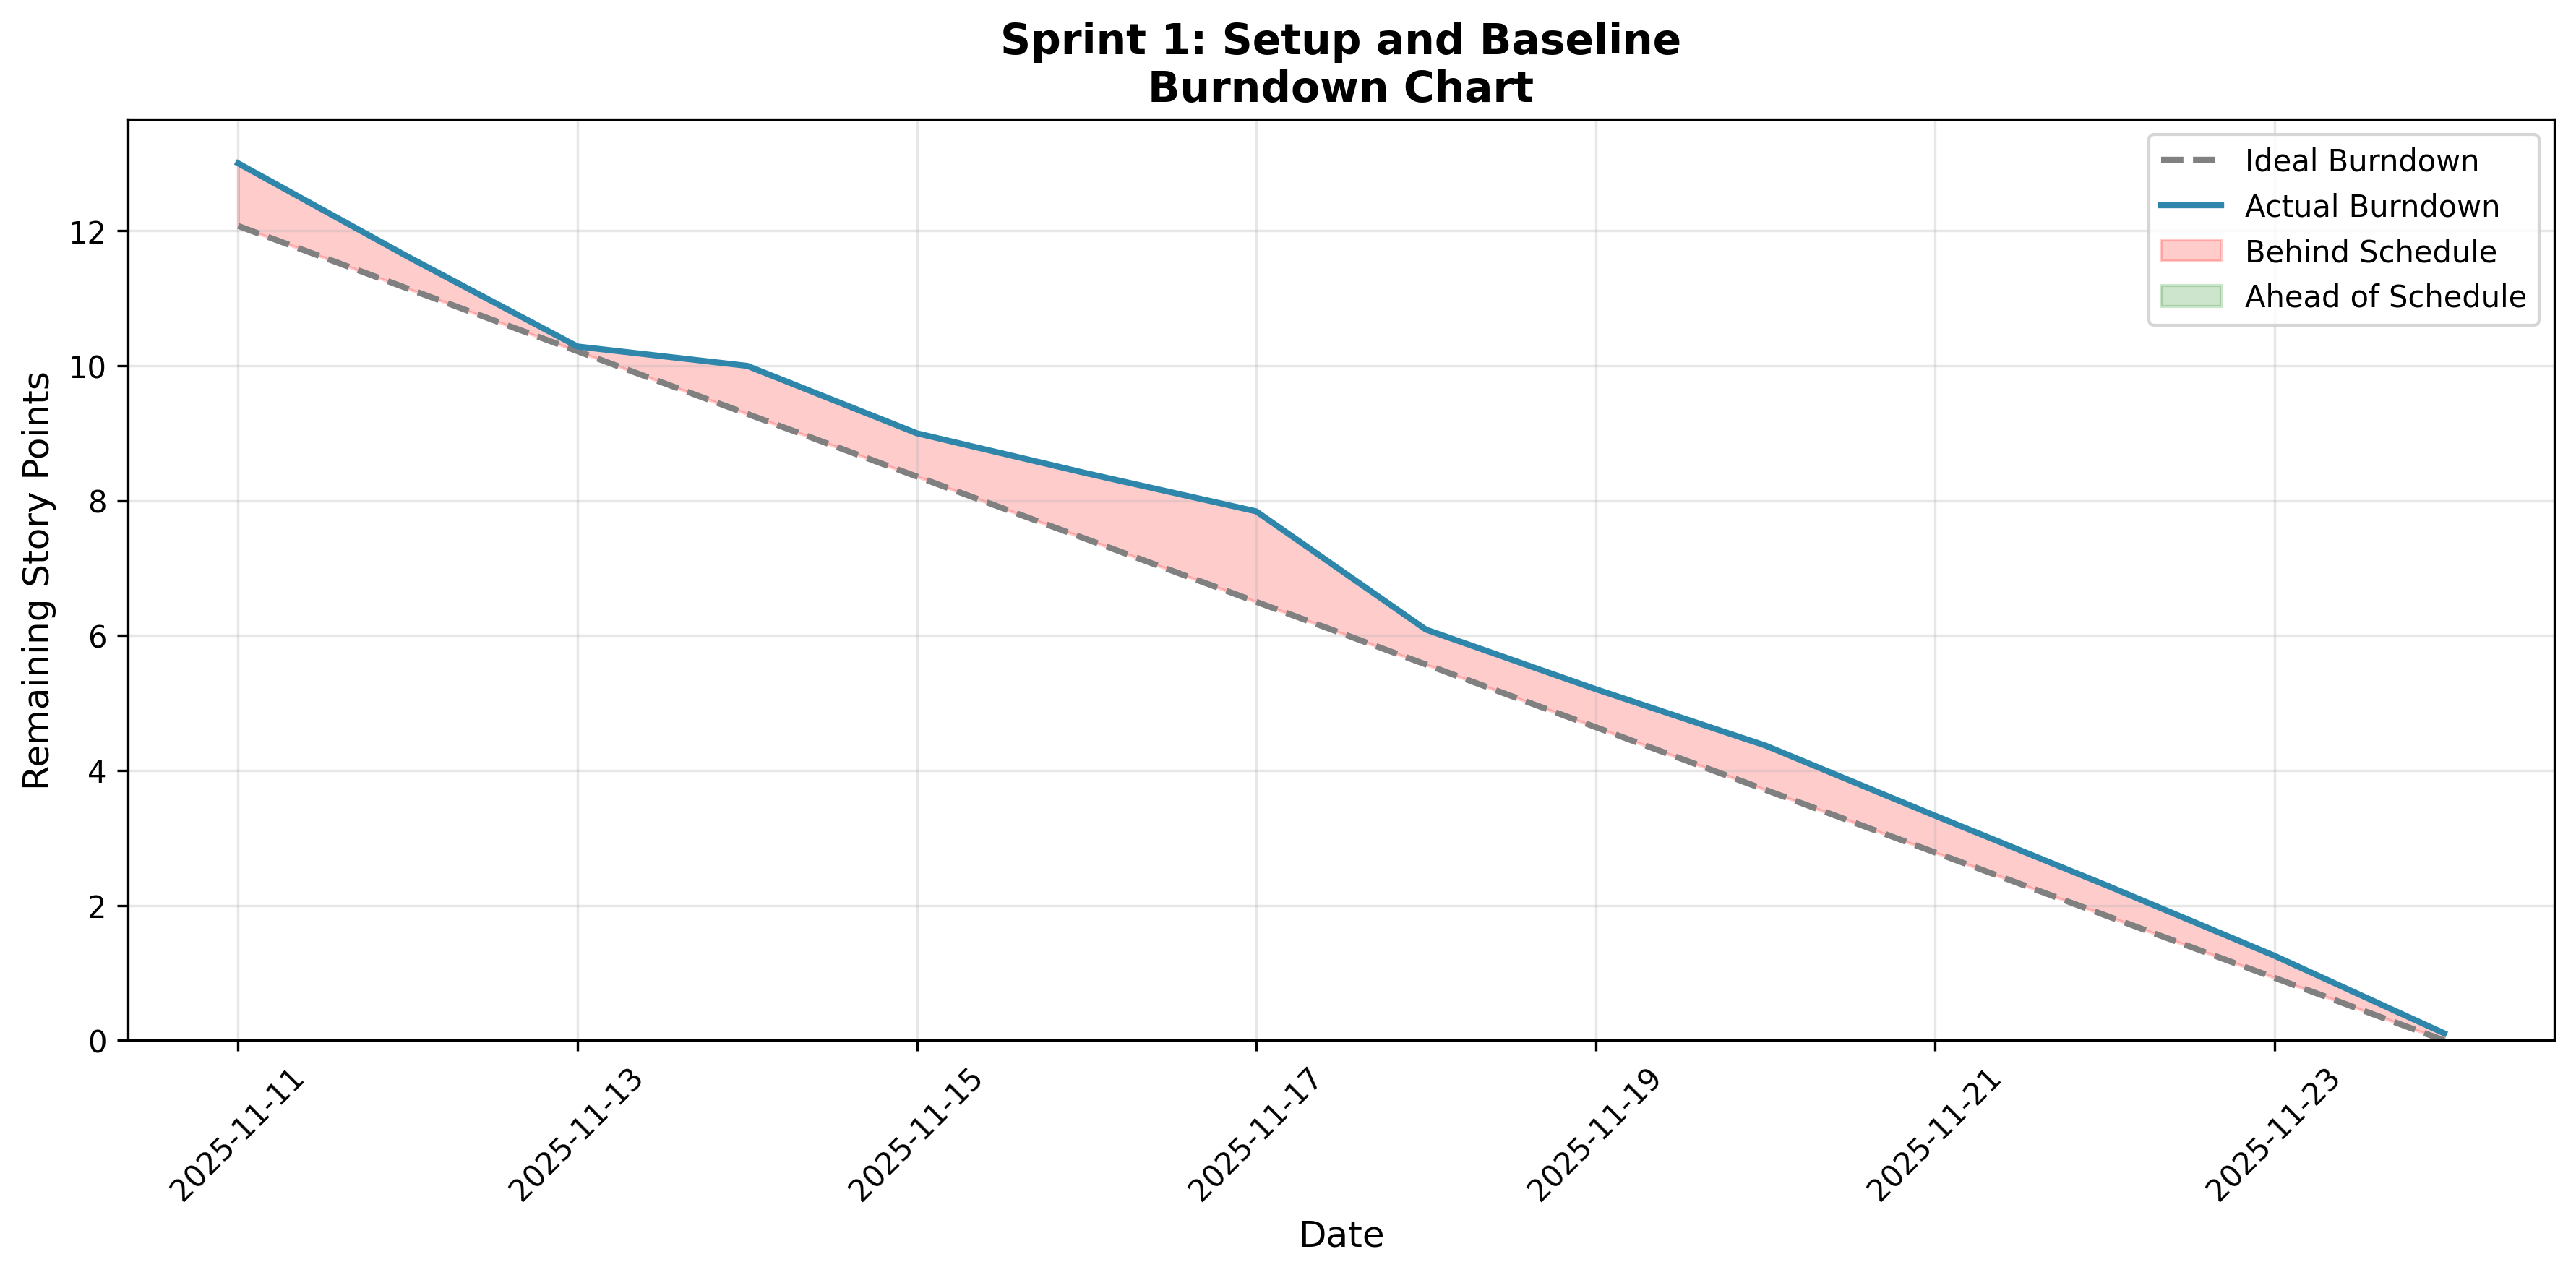
\includegraphics[width=0.8\textwidth]{temp/burndown_sprint_1.png}
\caption{Sprint 1 Burndown Chart: Progress tracking for project setup and baseline establishment (13 SP).}
\label{fig:burndown_sprint1}
\end{figure}

\textbf{Sprint 2 Burndown (Nov 23-30, 2025):}
Figure~\ref{fig:burndown_sprint2} demonstrates the burndown for Sprint 2, the largest sprint with 55 story points covering Phase 1 and Phase 1.5 implementations. Despite the high workload, the team successfully completed all planned work.

\begin{figure}[H]
\centering
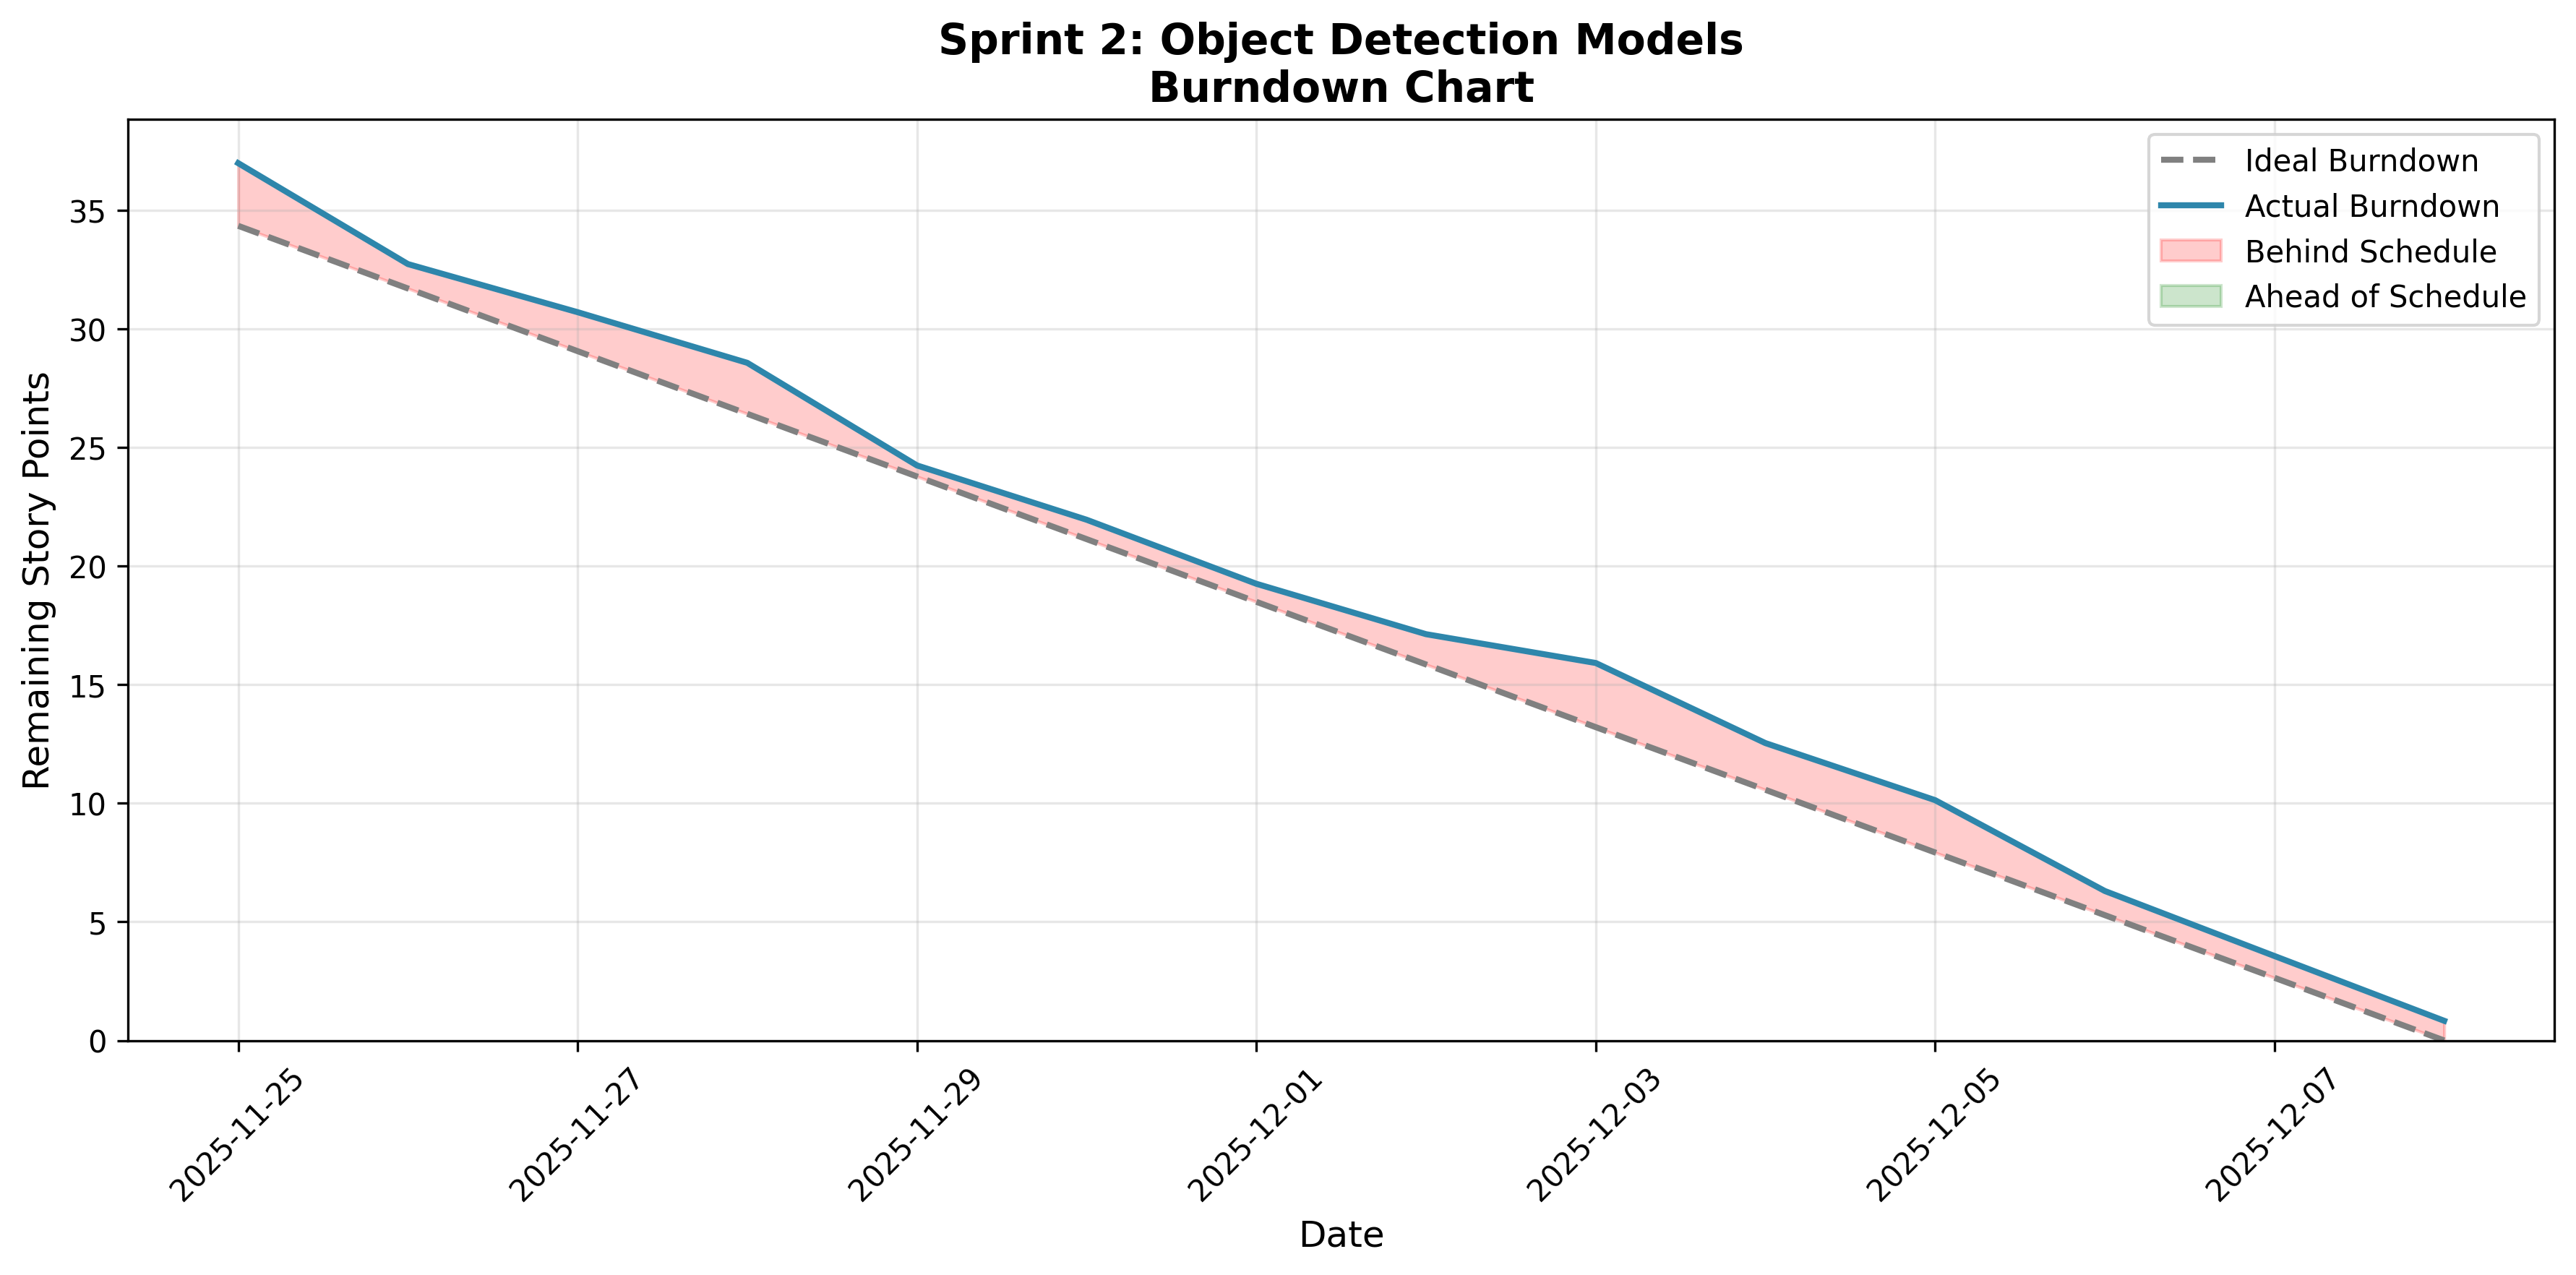
\includegraphics[width=0.8\textwidth]{temp/burndown_sprint_2.png}
\caption{Sprint 2 Burndown Chart: Progress tracking for Phase 1 and Phase 1.5 implementation (55 SP).}
\label{fig:burndown_sprint2}
\end{figure}

\textbf{Sprint 3 Burndown (Dec 1-7, 2025):}
Figure~\ref{fig:burndown_sprint3} shows the final sprint burndown, covering Phase 2 optimization, deployment, and report writing. The team maintained high velocity to complete all 50 story points.

\begin{figure}[H]
\centering
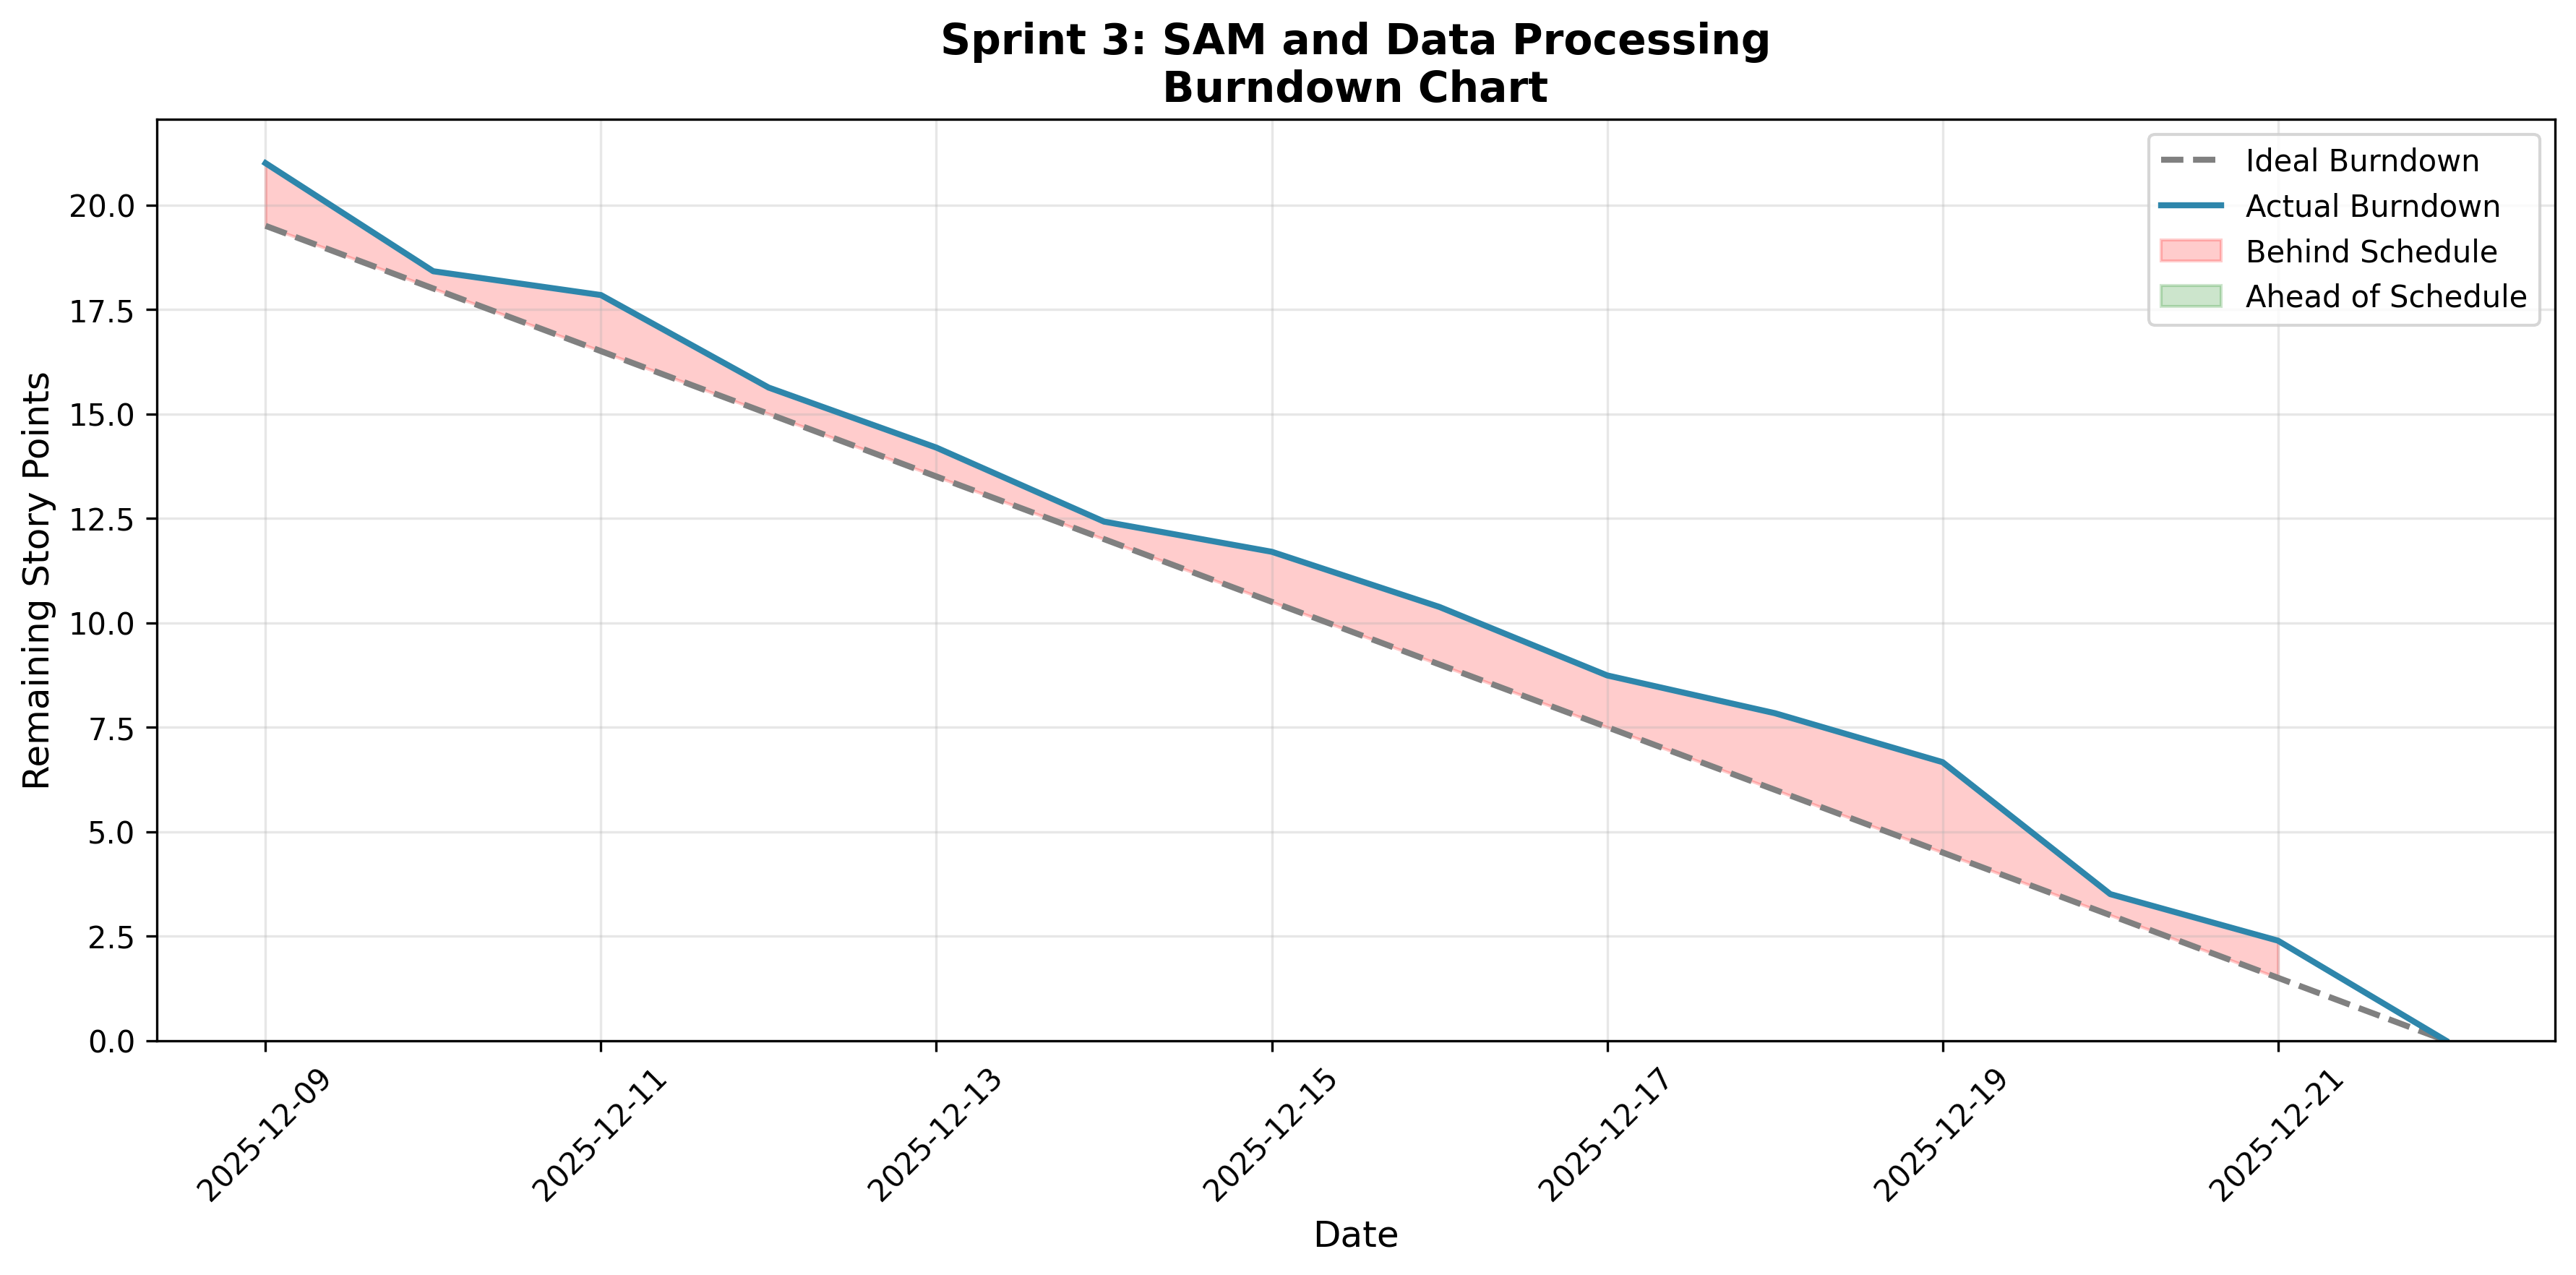
\includegraphics[width=0.8\textwidth]{temp/burndown_sprint_3.png}
\caption{Sprint 3 Burndown Chart: Progress tracking for Phase 2 optimization, deployment, and report writing (50 SP).}
\label{fig:burndown_sprint3}
\end{figure}

\textbf{Overall Project Burndown:}
Figure~\ref{fig:burndown_overall} provides a comprehensive view of the entire project's progress, showing the completion of all 118 story points across three sprints.

\begin{figure}[H]
\centering
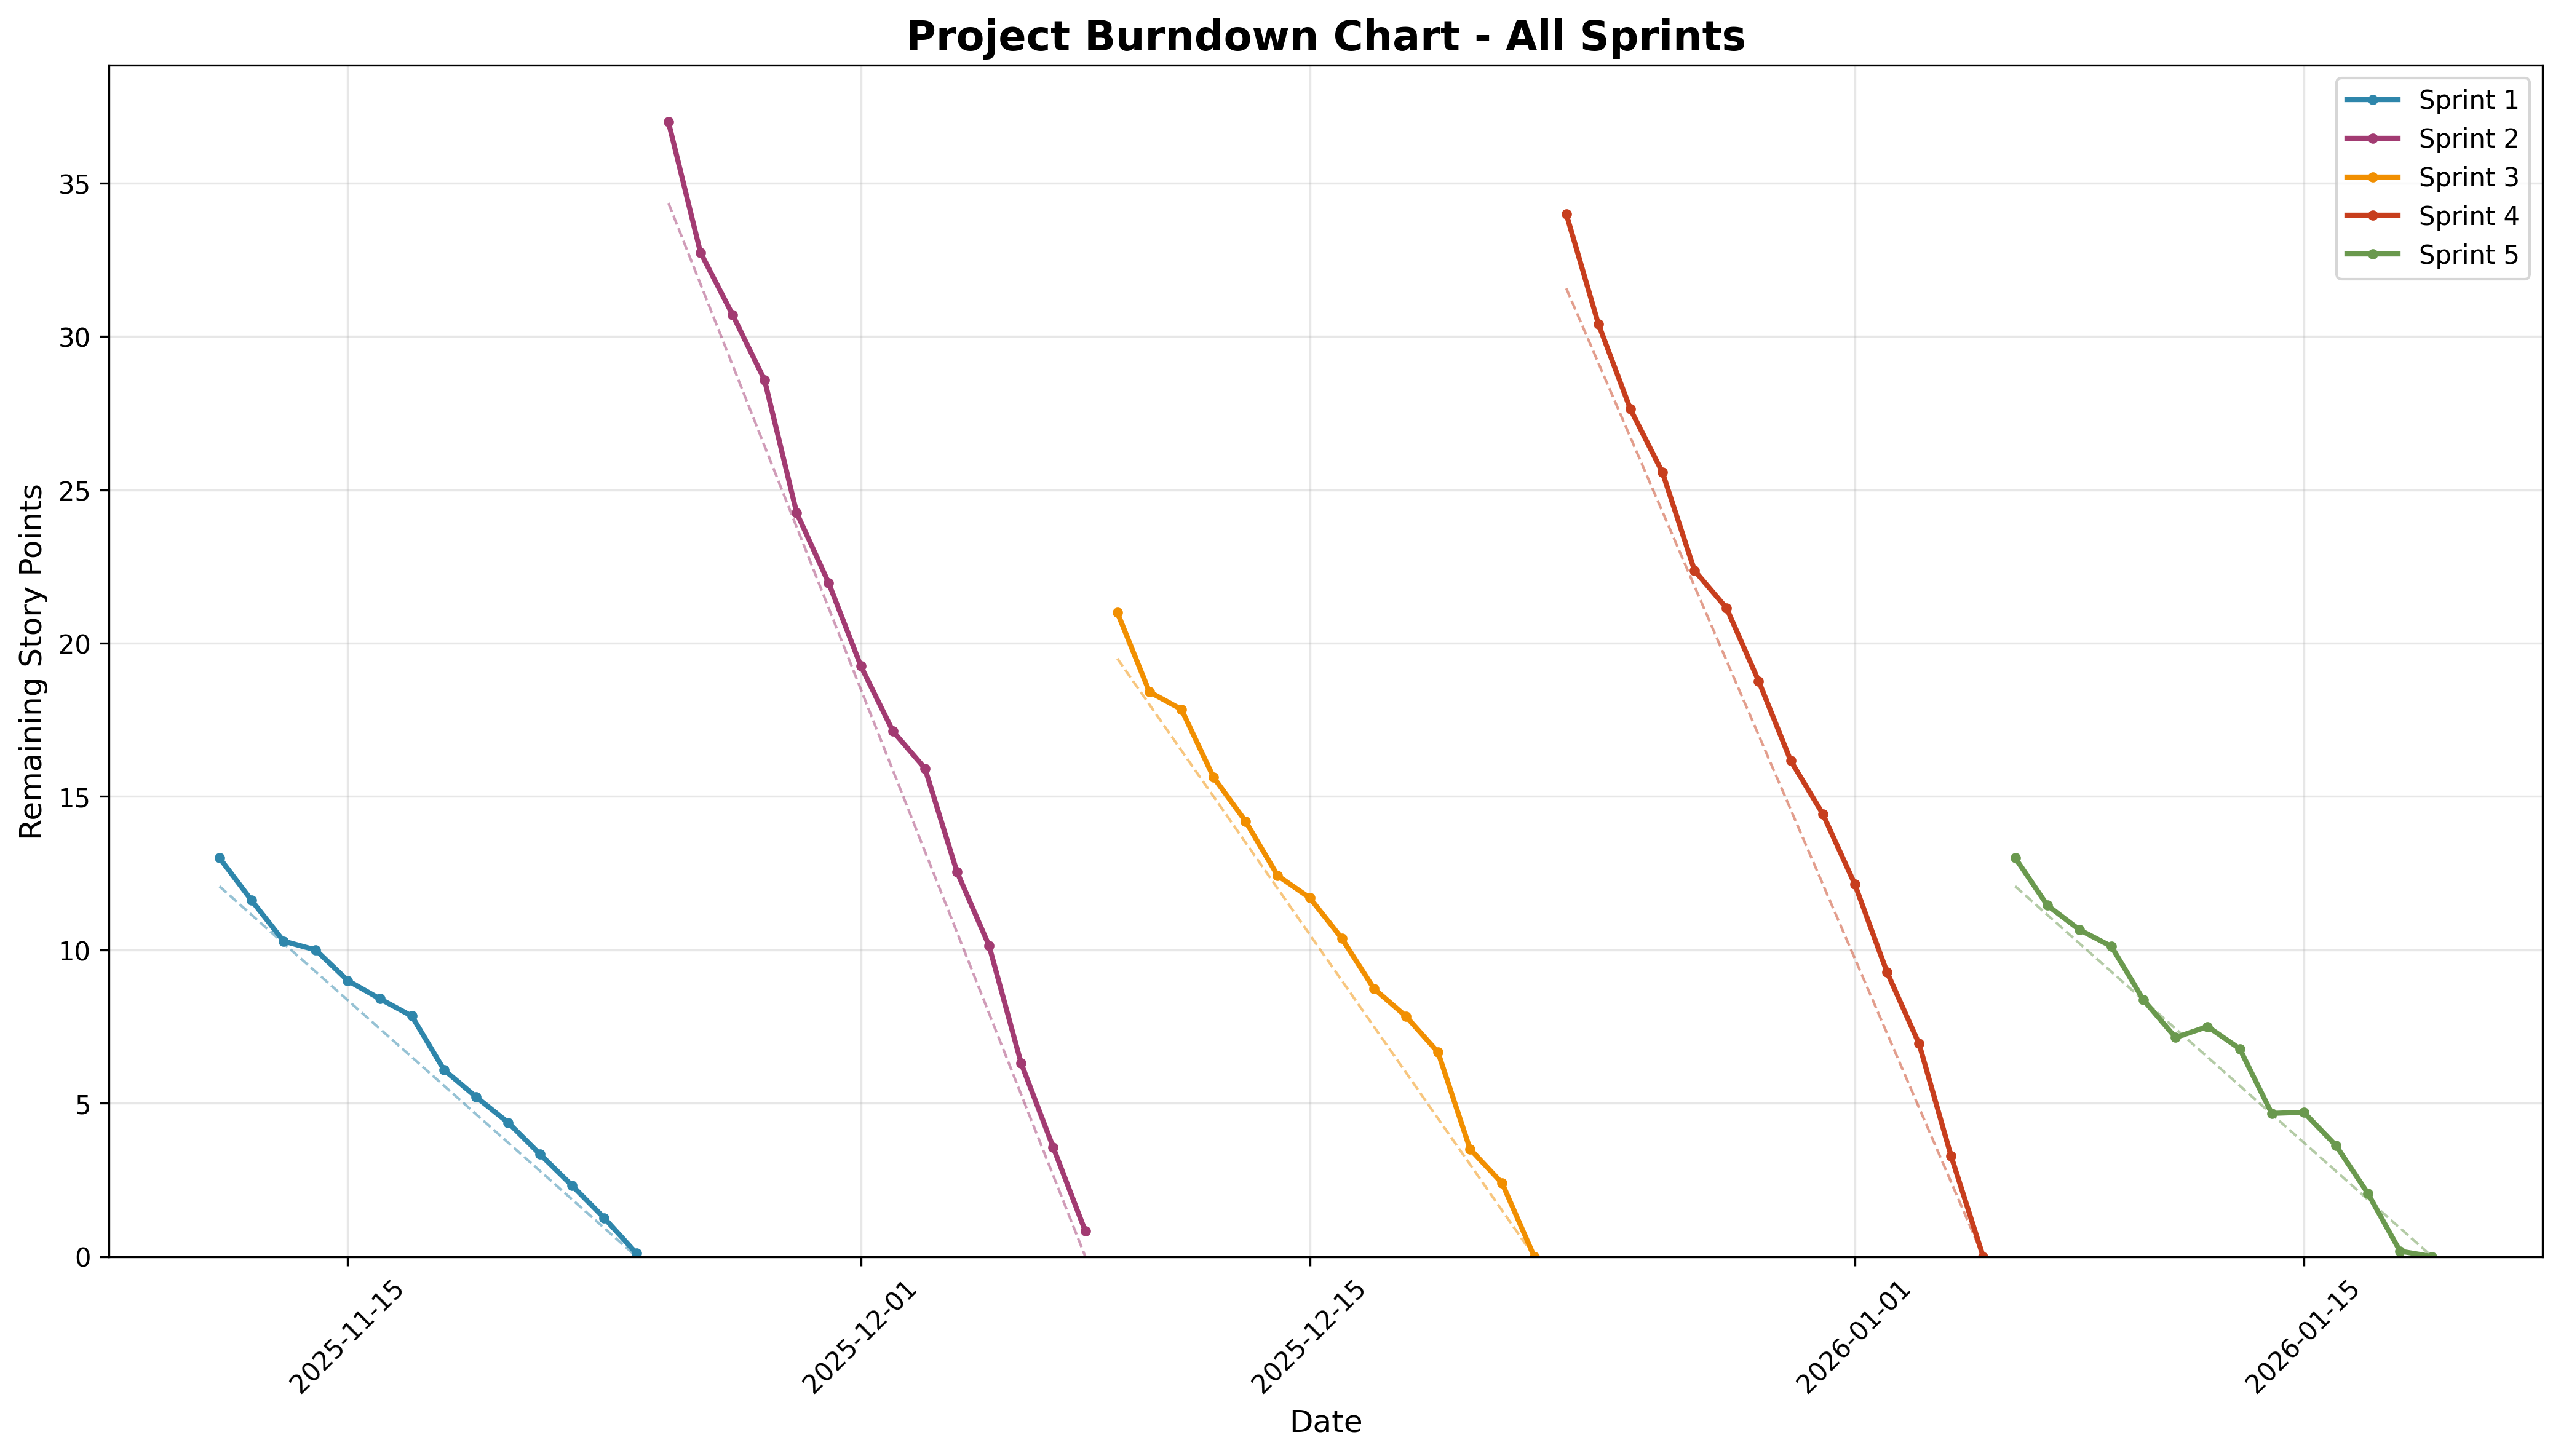
\includegraphics[width=0.8\textwidth]{temp/burndown_project_overall.png}
\caption{Overall Project Burndown Chart: Complete project progress showing all 118 story points completed across three sprints.}
\label{fig:burndown_overall}
\end{figure}

\subsection{Scrum Board and Task Management}

The project utilized a Scrum board to track tasks across different stages: To Do, In Progress, and Done. Figure~\ref{fig:scrum_board} shows the Scrum board visualization, demonstrating the organization of work items across epics and sprints.

\begin{figure}[H]
\centering
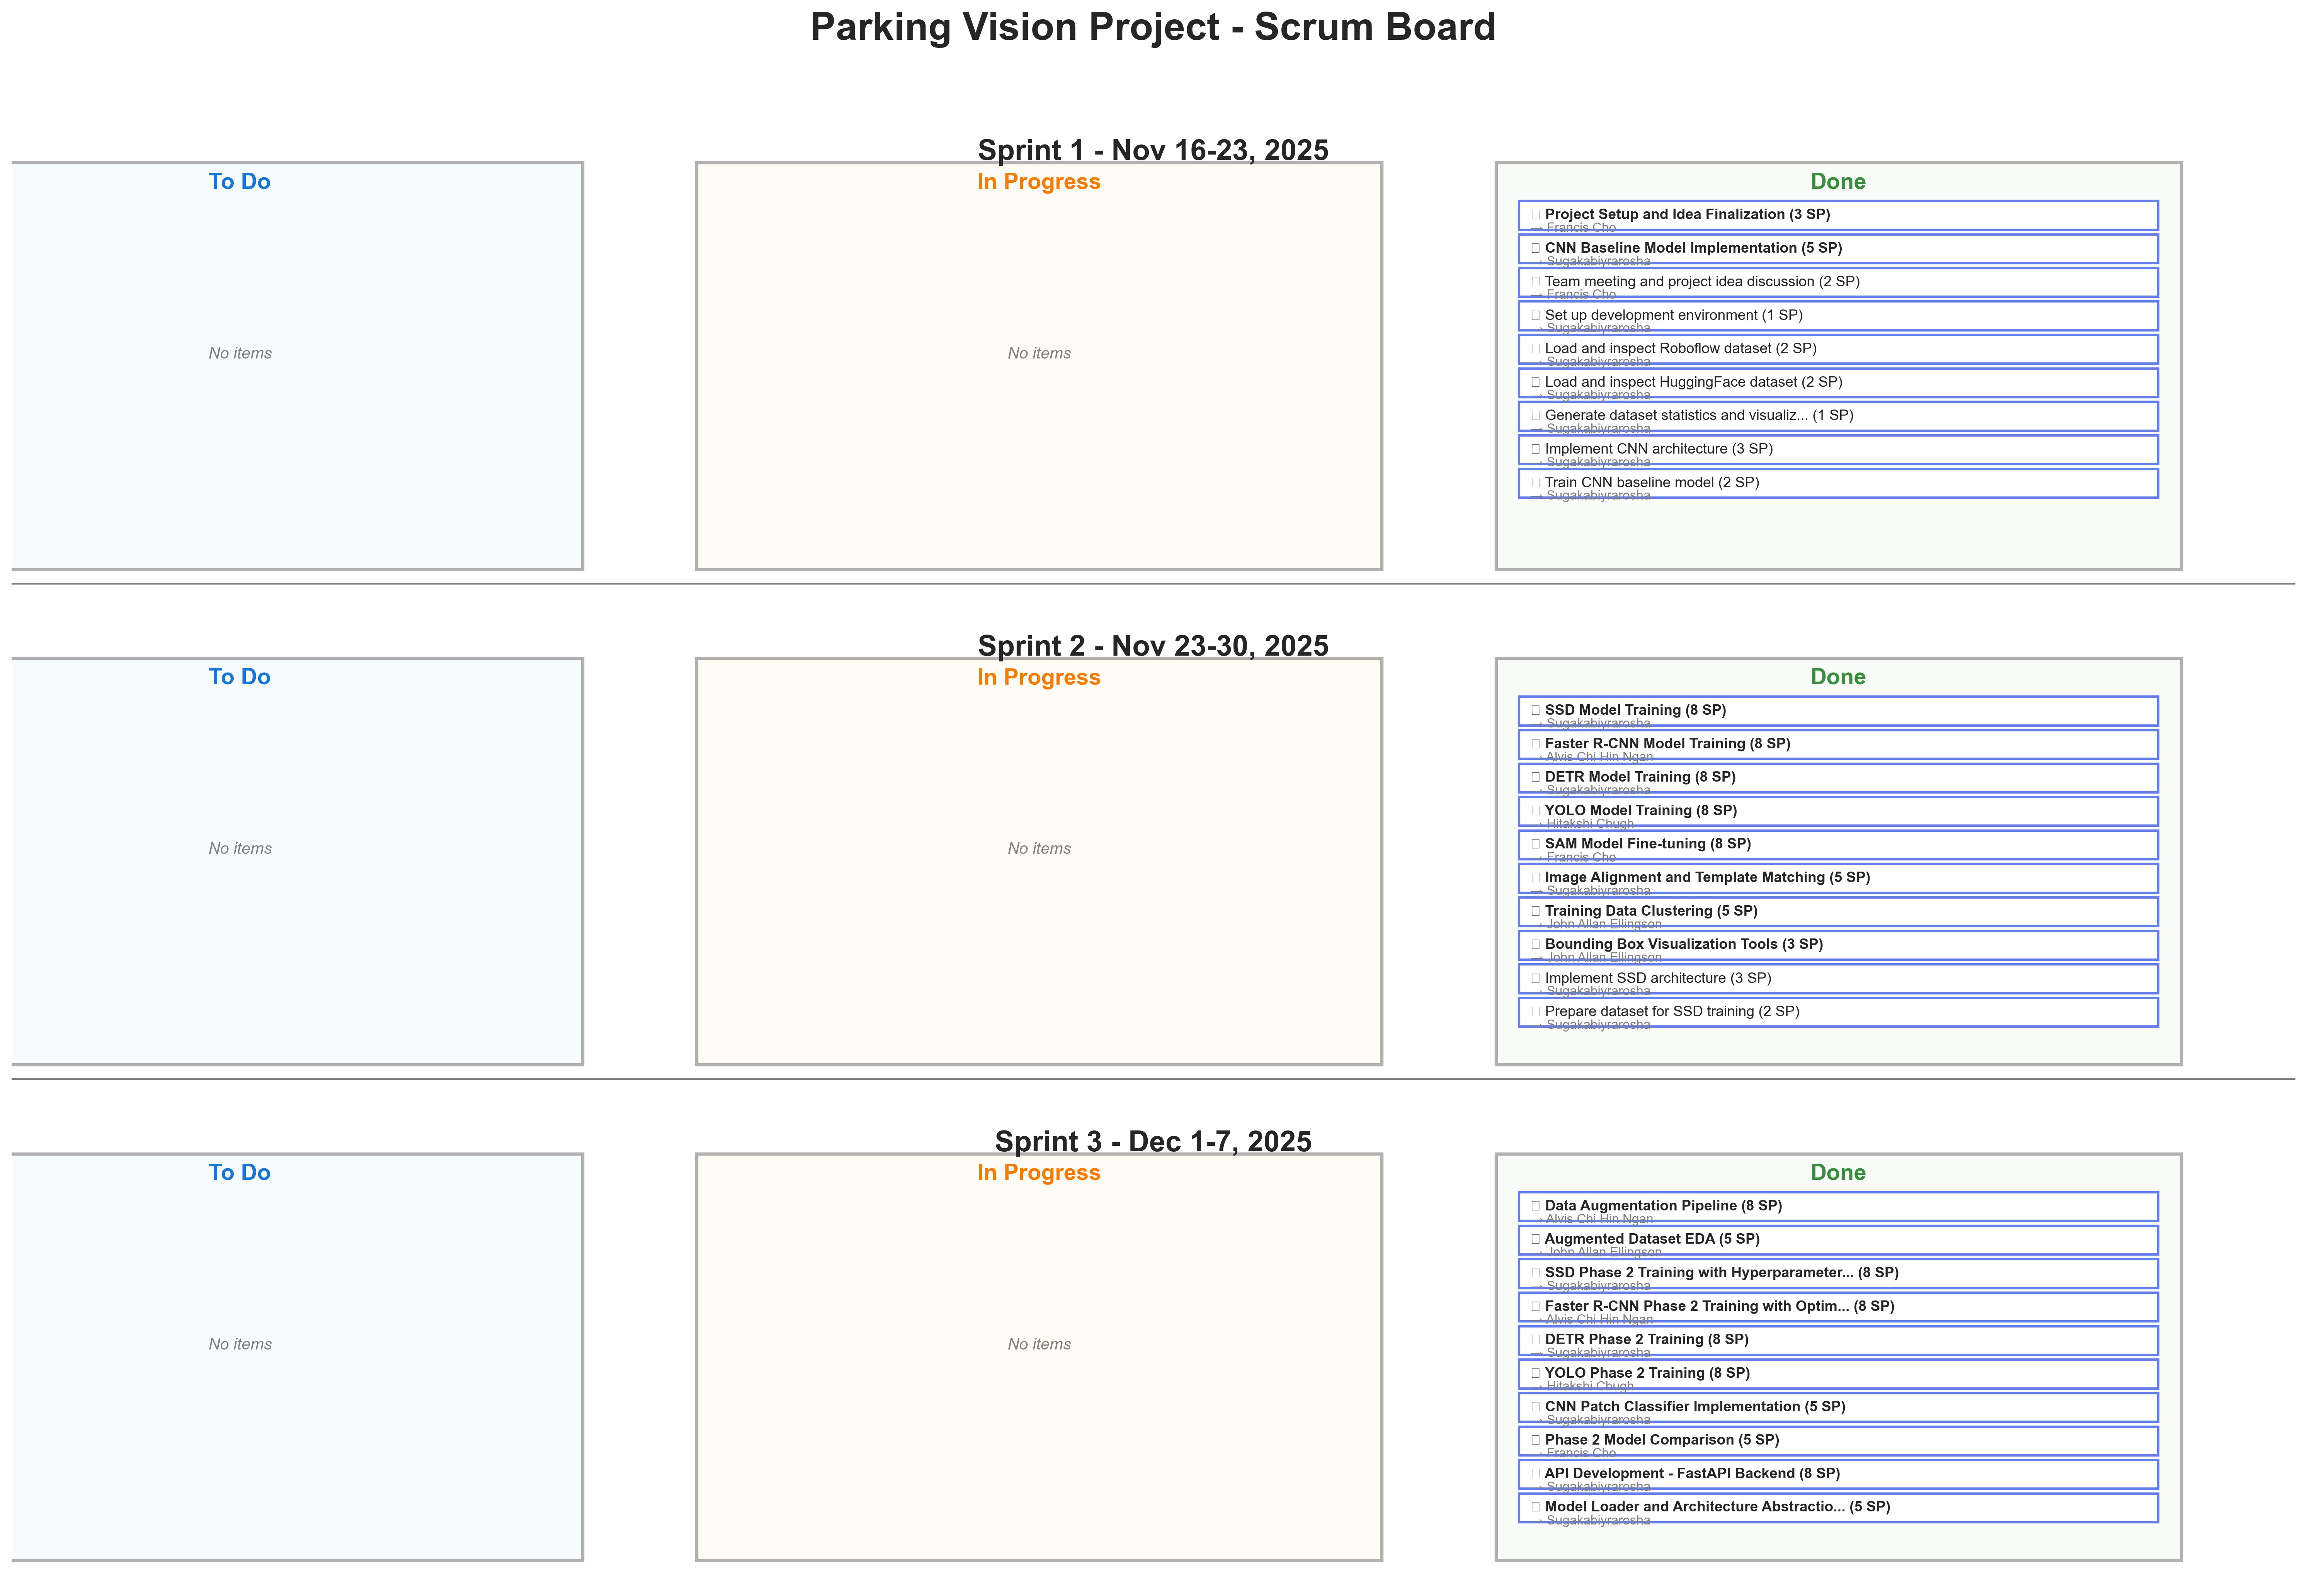
\includegraphics[width=0.95\textwidth]{temp/scrum_board.png}
\caption{Scrum Board: Task organization showing Epics, User Stories, and Tasks across different stages (To Do, In Progress, Done).}
\label{fig:scrum_board}
\end{figure}

The Scrum board includes:
\begin{itemize}
    \item \textbf{4 Epics:} Phase 1, Phase 1.5, Phase 2, and Deployment
    \item \textbf{25 User Stories:} Detailed feature requirements
    \item \textbf{90+ Tasks:} Granular work items assigned to team members
    \item \textbf{Status Tracking:} Visual representation of work progress
\end{itemize}

\subsection{Team Workload Distribution}

Figure~\ref{fig:team_workload} illustrates the distribution of work across team members, showing how tasks were allocated based on expertise and availability. The chart demonstrates balanced workload distribution and effective team collaboration.

\begin{figure}[H]
\centering
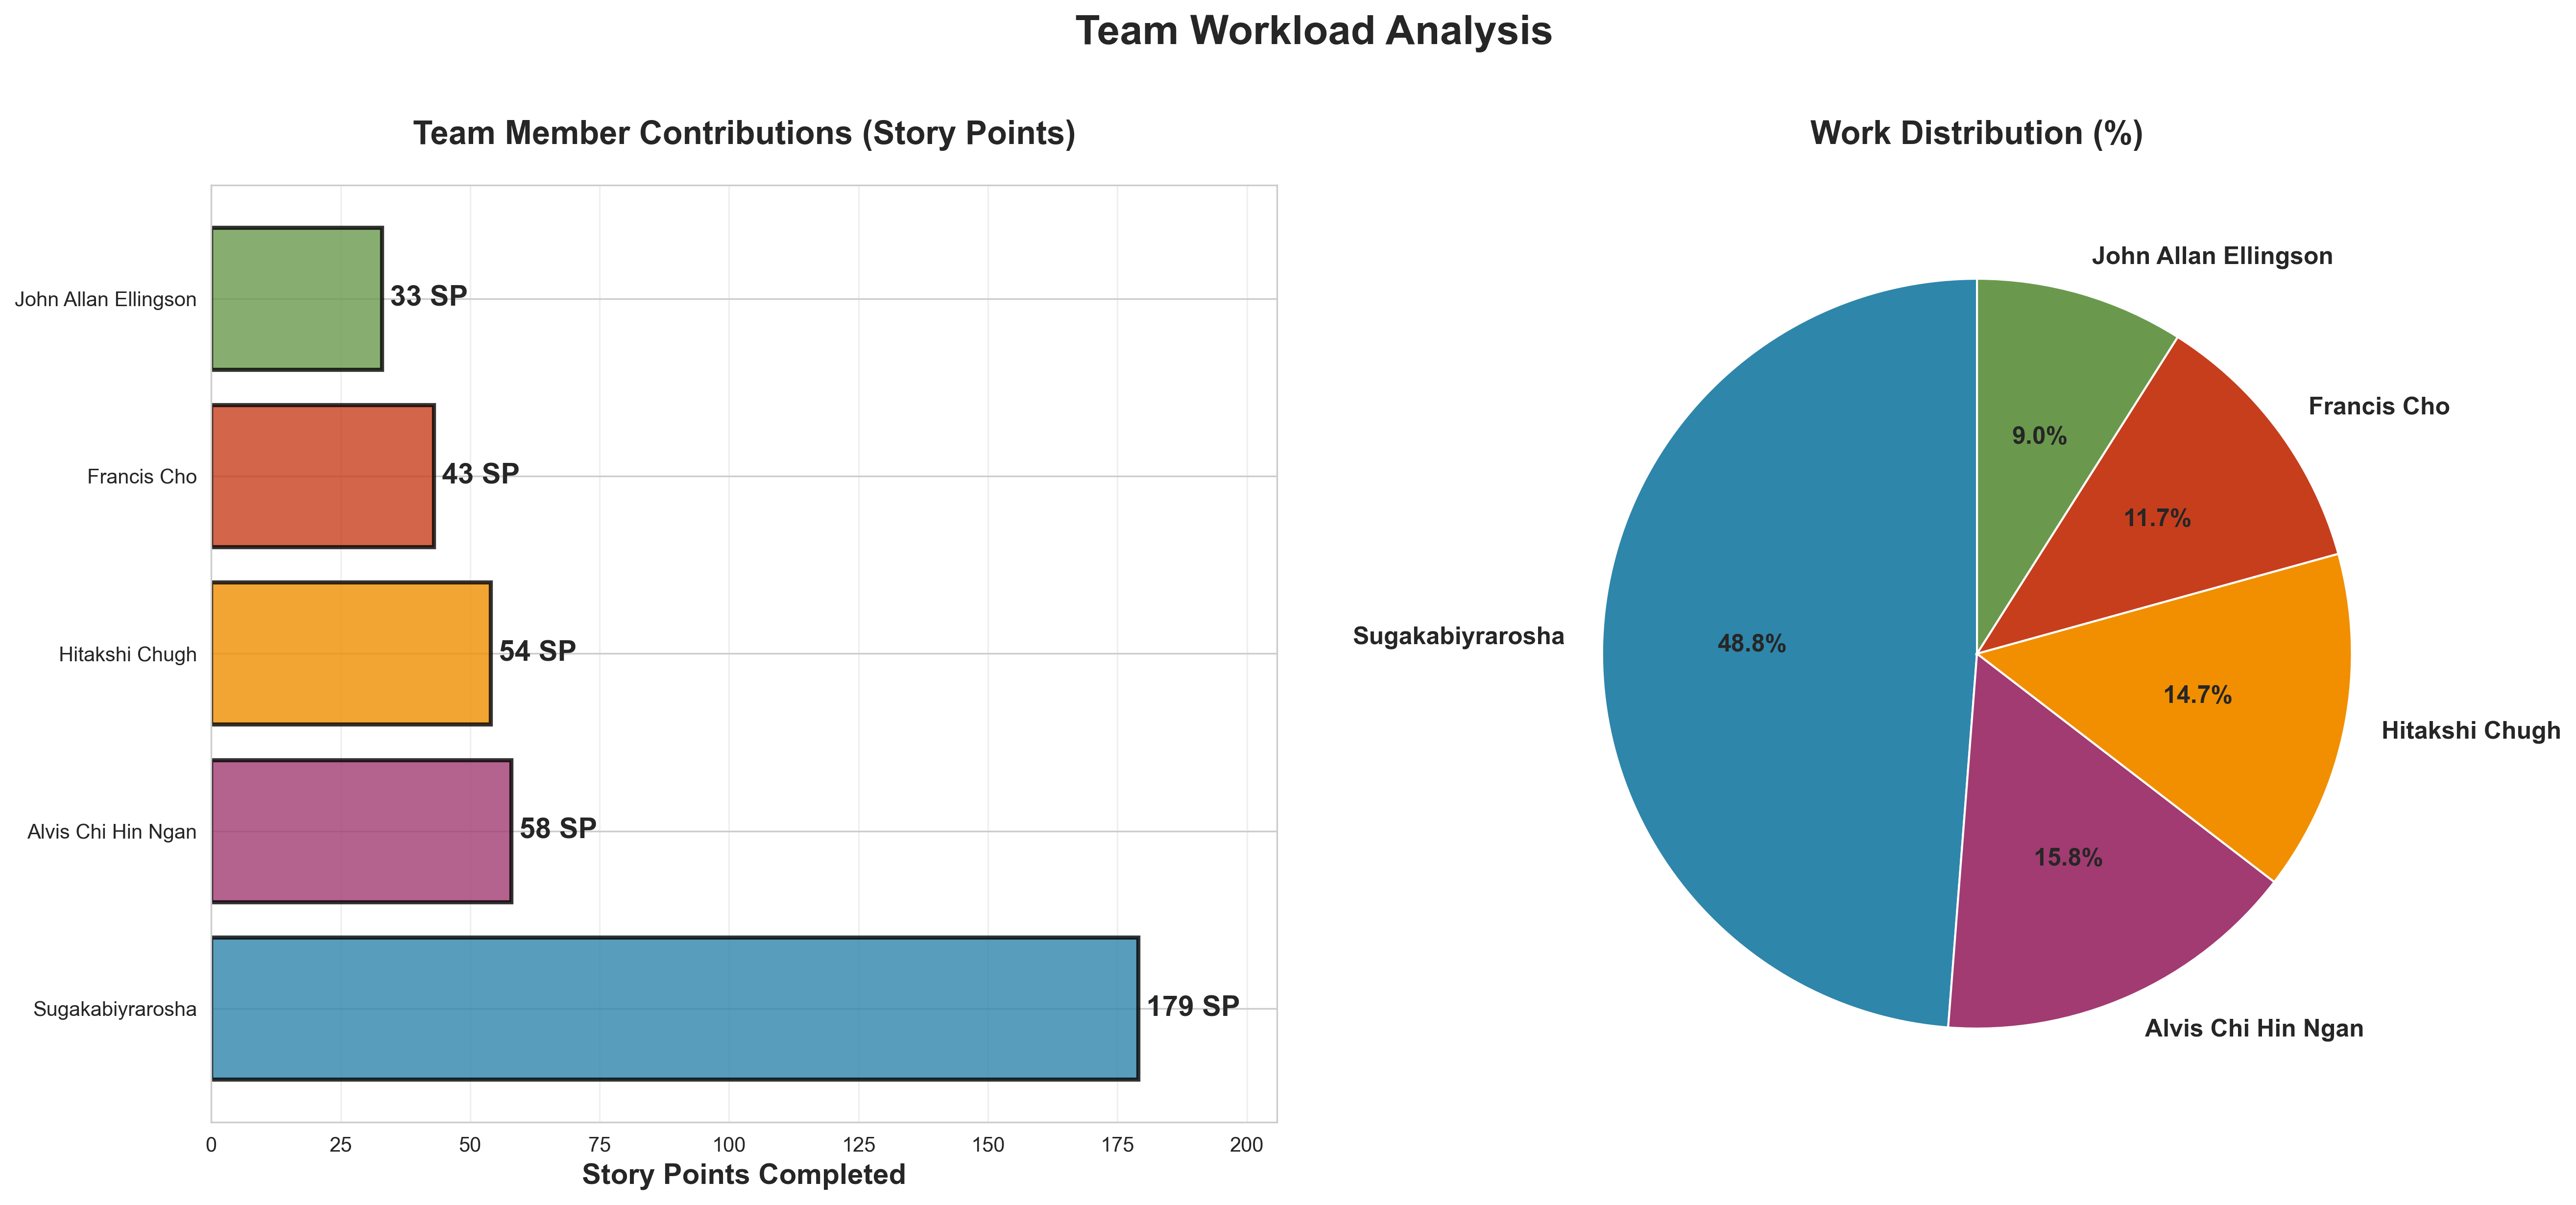
\includegraphics[width=0.9\textwidth]{temp/team_workload.png}
\caption{Team Workload Distribution: Visualization of work allocation across team members showing balanced distribution and collaboration.}
\label{fig:team_workload}
\end{figure}

\subsection{Epic Summary}

Figure~\ref{fig:epic_summary} provides an overview of all four epics, showing the breakdown of story points and progress across different project phases.

\begin{figure}[H]
\centering
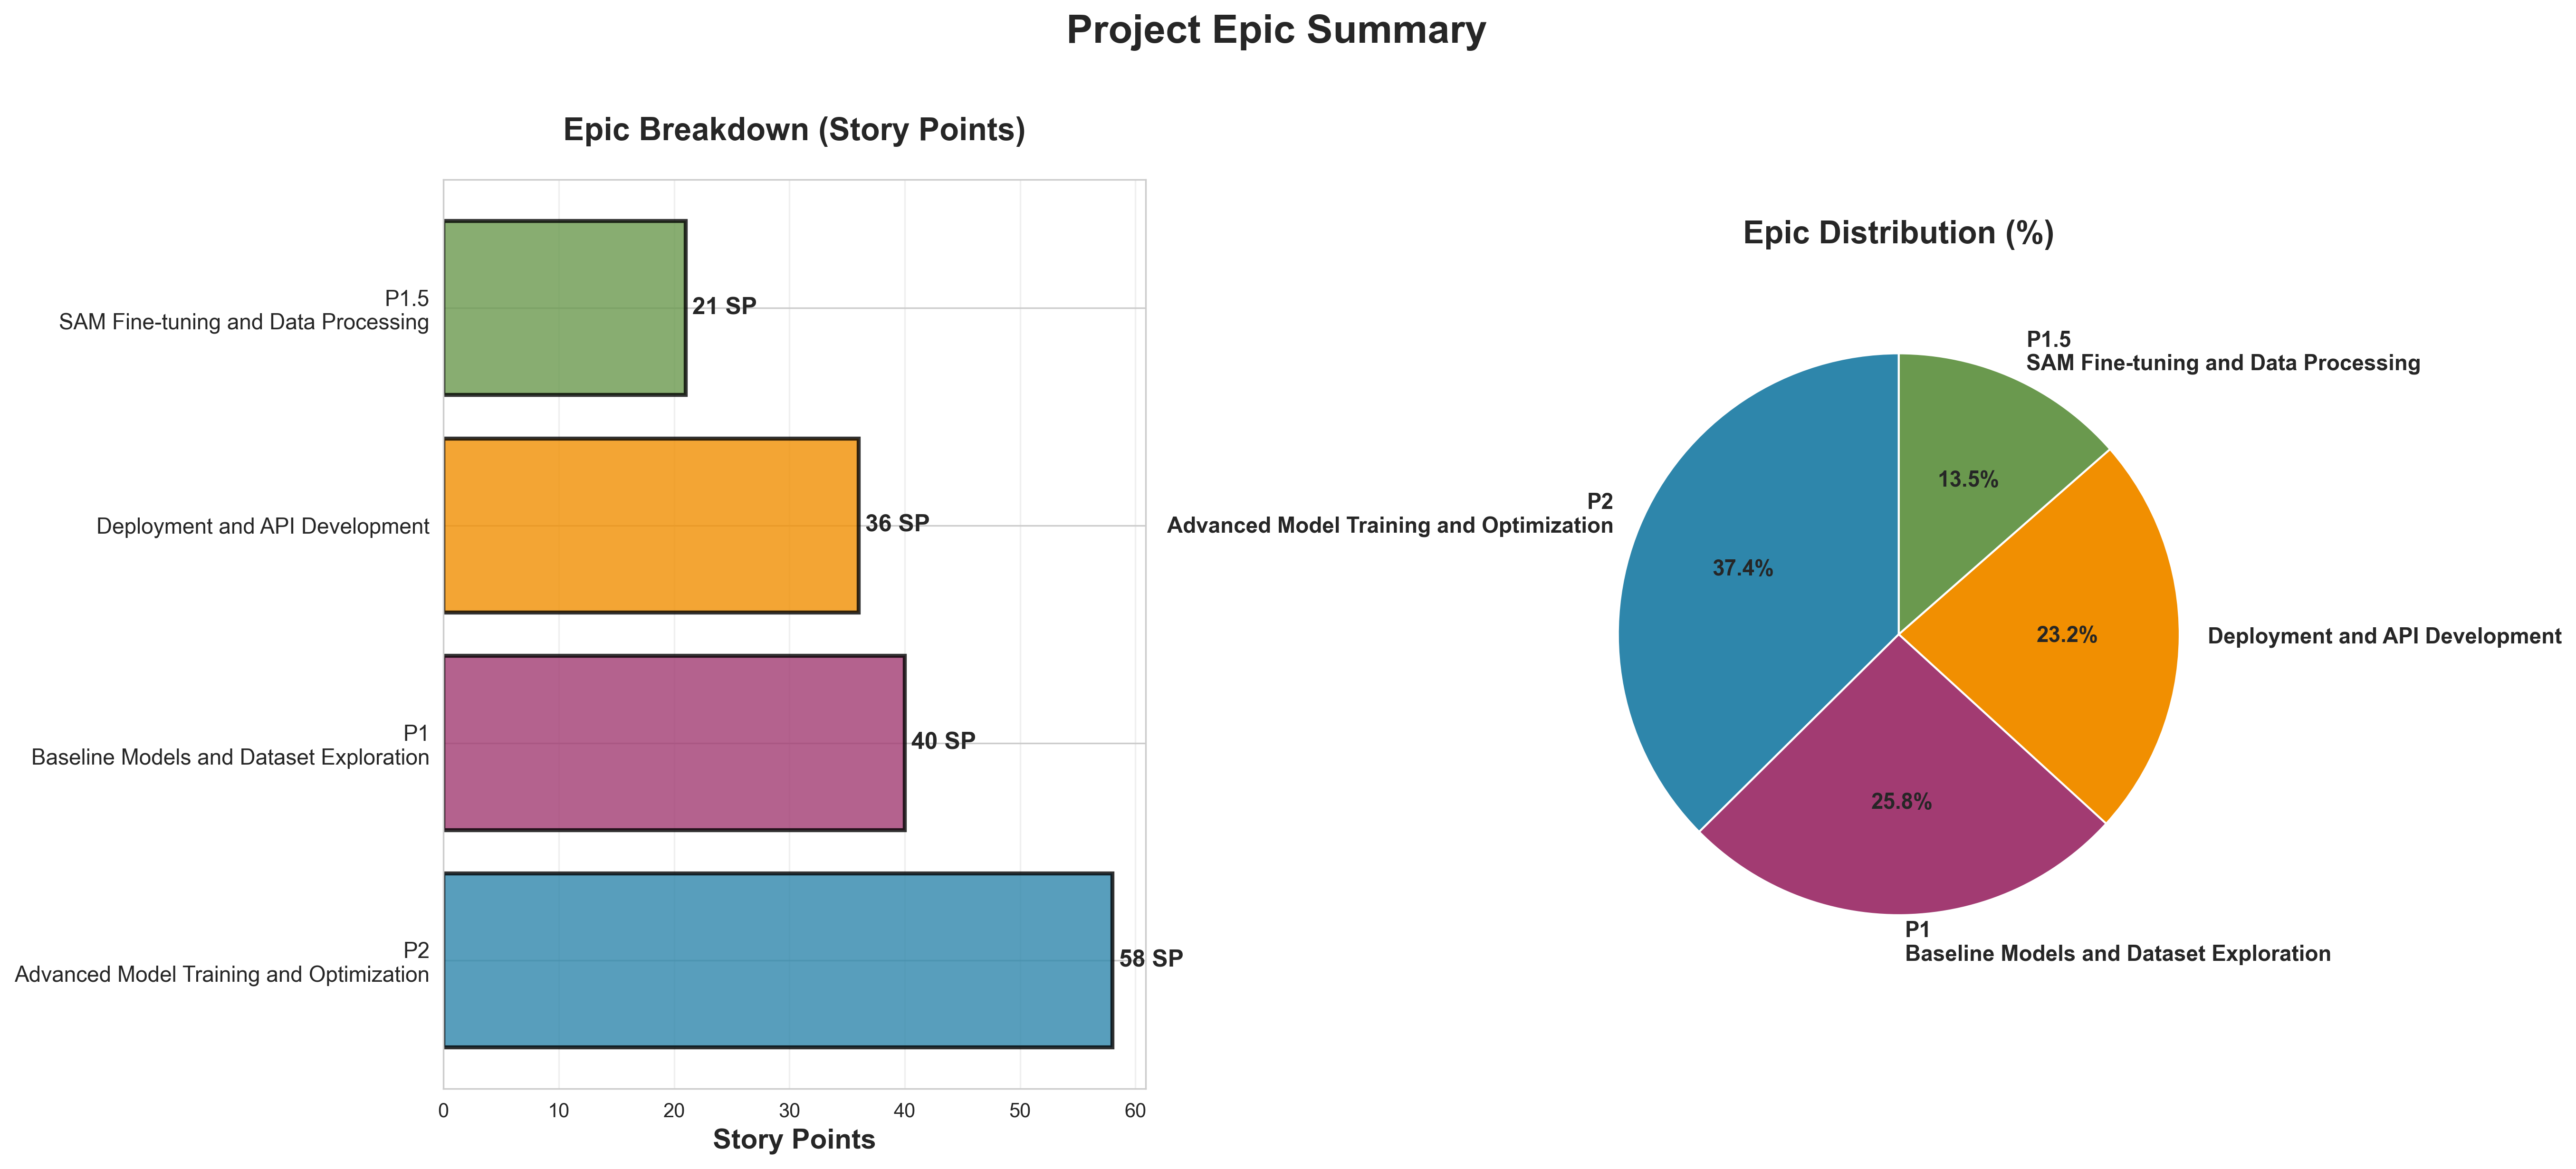
\includegraphics[width=0.9\textwidth]{temp/epic_summary.png}
\caption{Epic Summary: Overview of all four project epics showing story point distribution and completion status.}
\label{fig:epic_summary}
\end{figure}

\subsection{Sprint Timeline}

Figure~\ref{fig:sprint_timeline} shows the chronological timeline of all sprints, highlighting key milestones and deliverables throughout the project duration.

\begin{figure}[H]
\centering
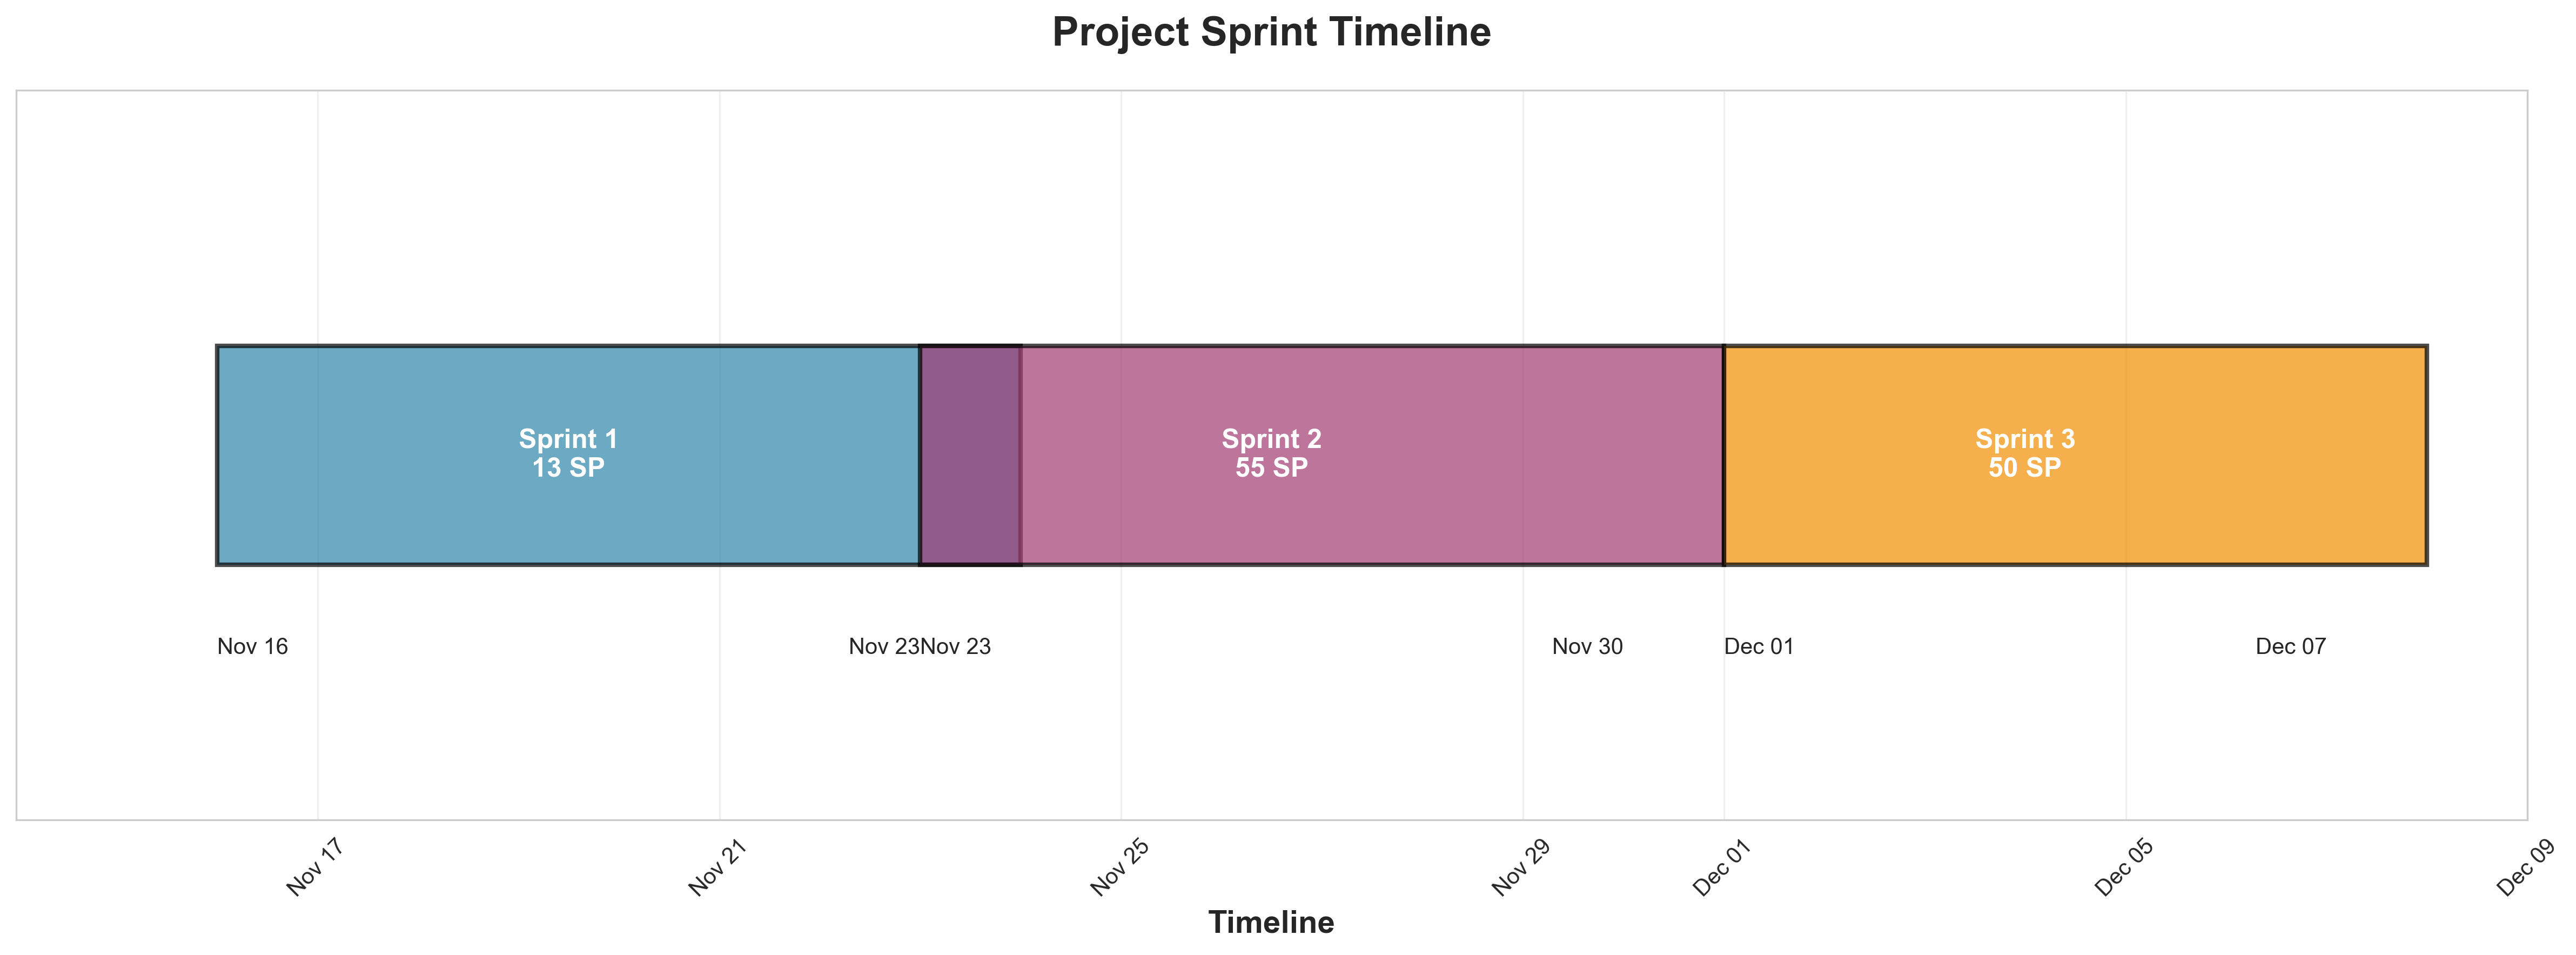
\includegraphics[width=0.9\textwidth]{temp/sprint_timeline.png}
\caption{Sprint Timeline: Chronological view of all three sprints with key milestones and deliverables.}
\label{fig:sprint_timeline}
\end{figure}

\subsection{Sprint Summaries}

Figure~\ref{fig:sprint_summary} provides a comprehensive summary table of all sprints, including story points, key deliverables, and completion status.

\begin{figure}[H]
\centering
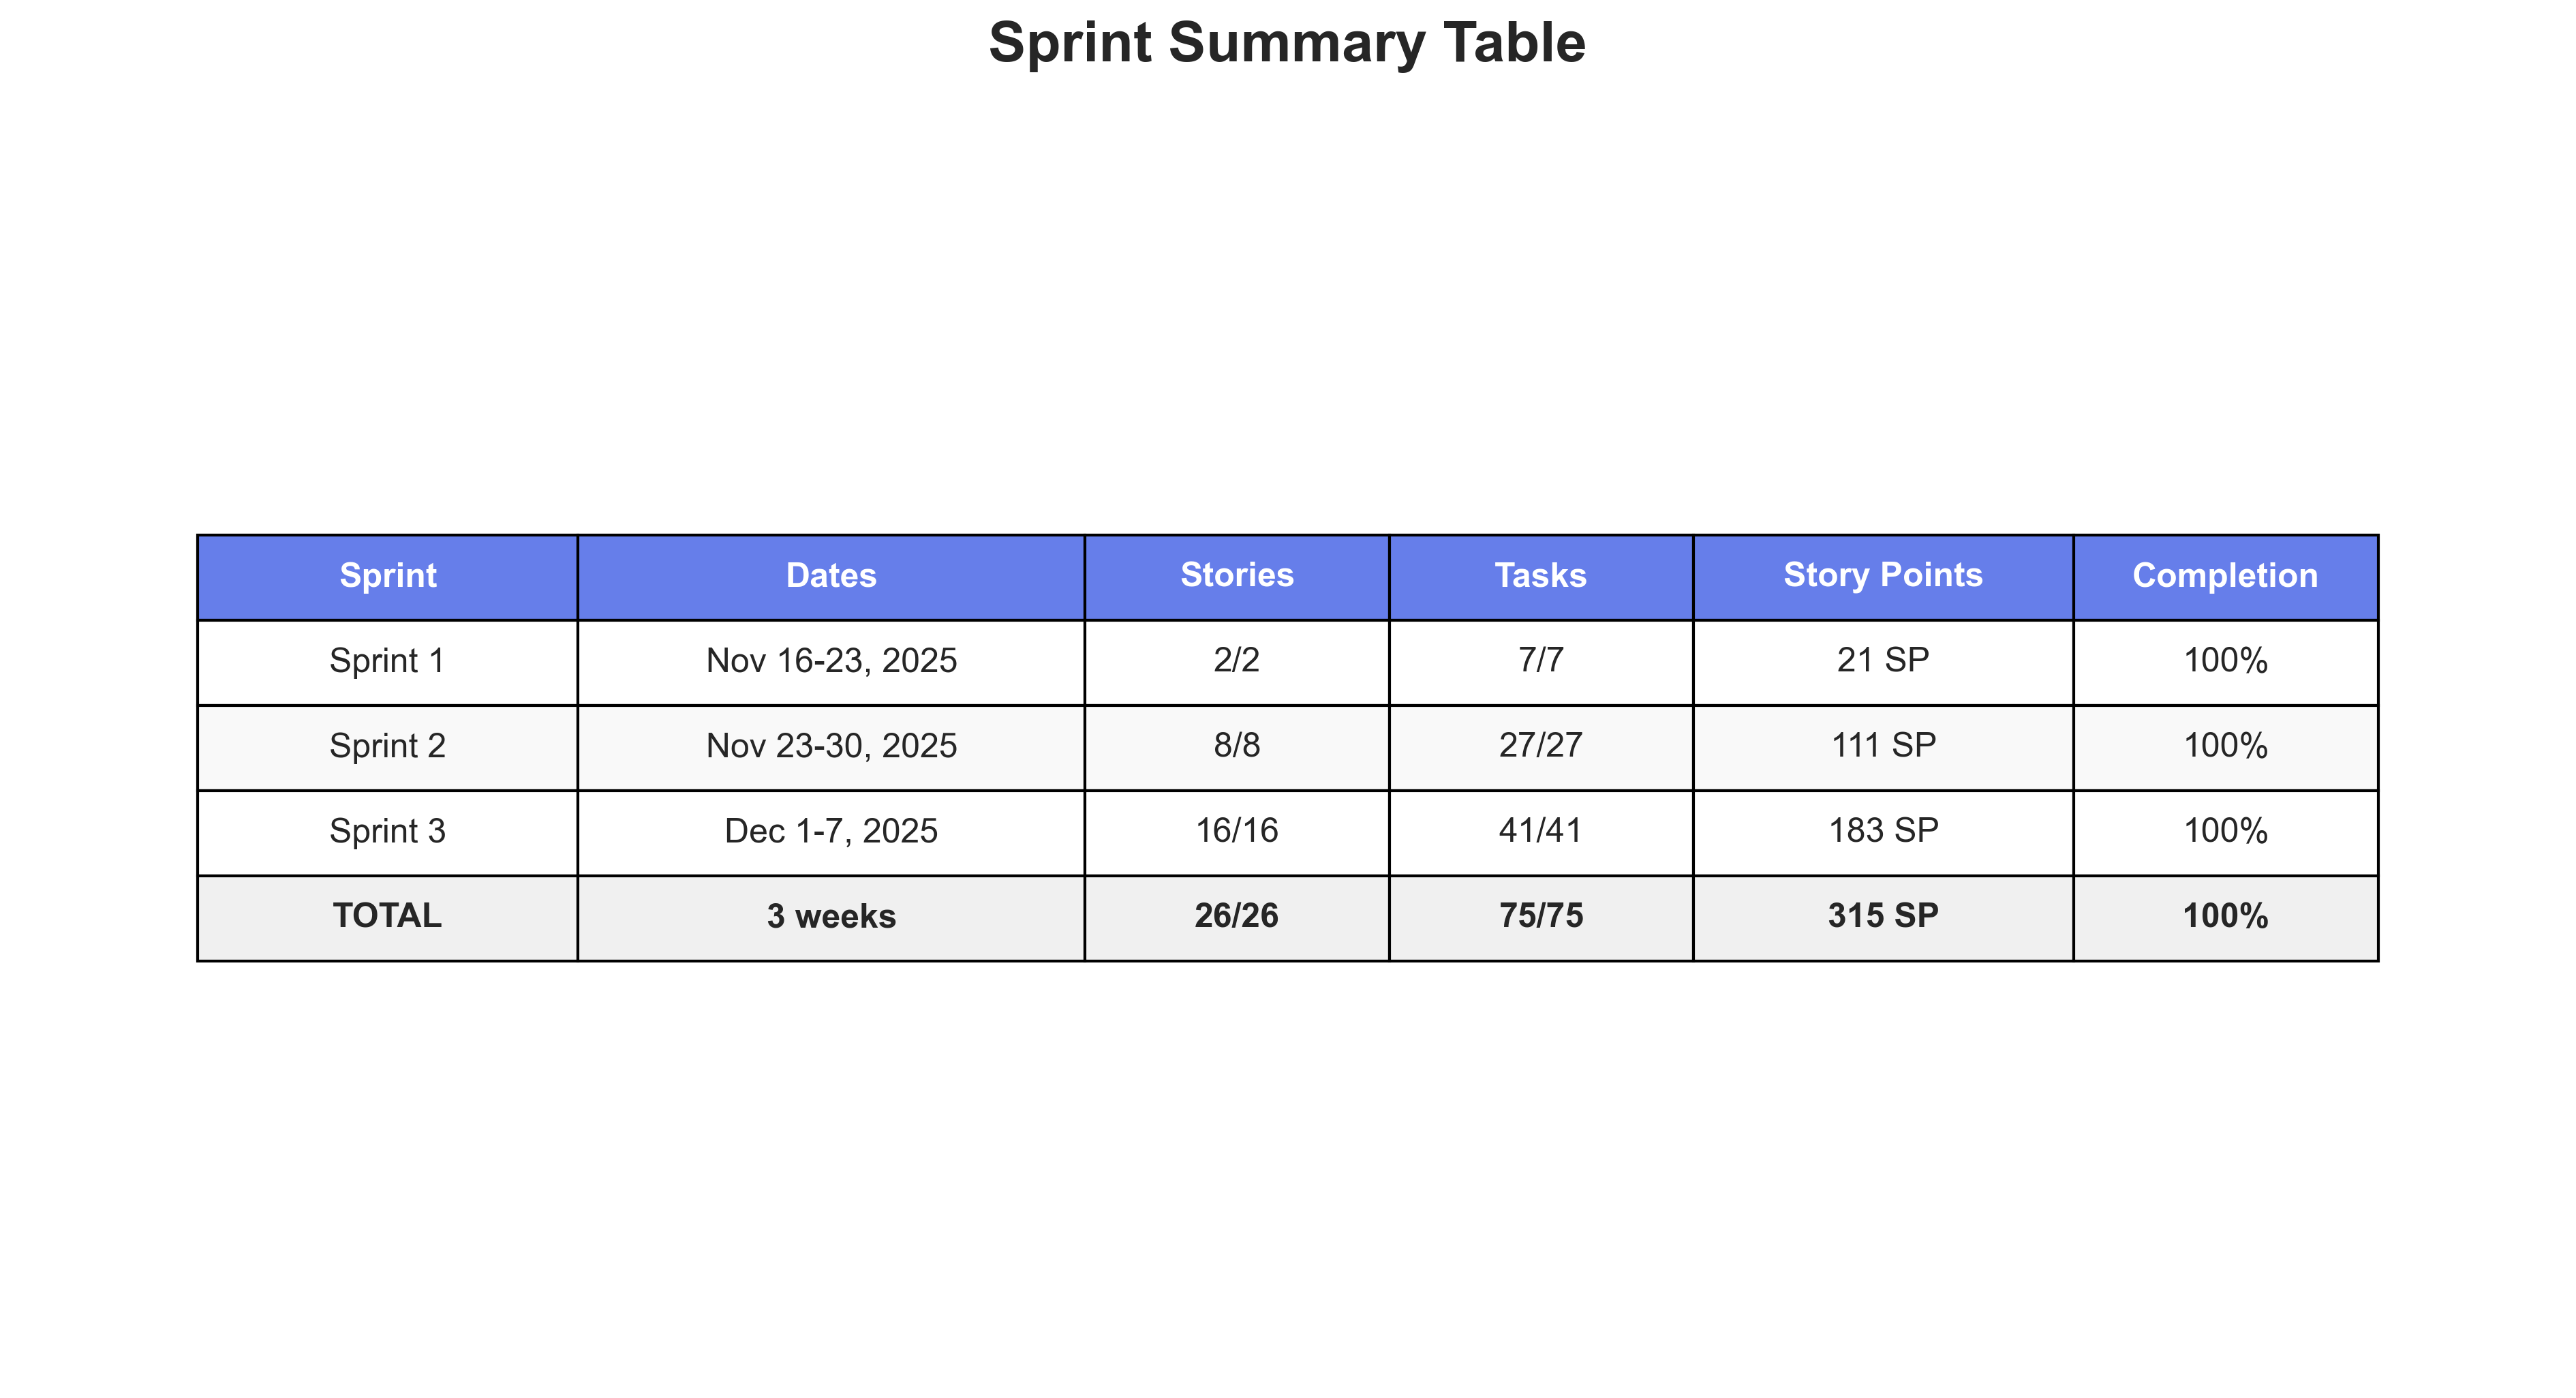
\includegraphics[width=0.9\textwidth]{temp/sprint_summary.png}
\caption{Sprint Summary: Comprehensive table showing all sprint details including story points, deliverables, and status.}
\label{fig:sprint_summary}
\end{figure}

\subsection{Team Contributions Visualization}

Figure~\ref{fig:team_contributions_chart} visualizes individual team member contributions across the project, showing the distribution of work and highlighting each member's key areas of responsibility.

\begin{figure}[H]
\centering
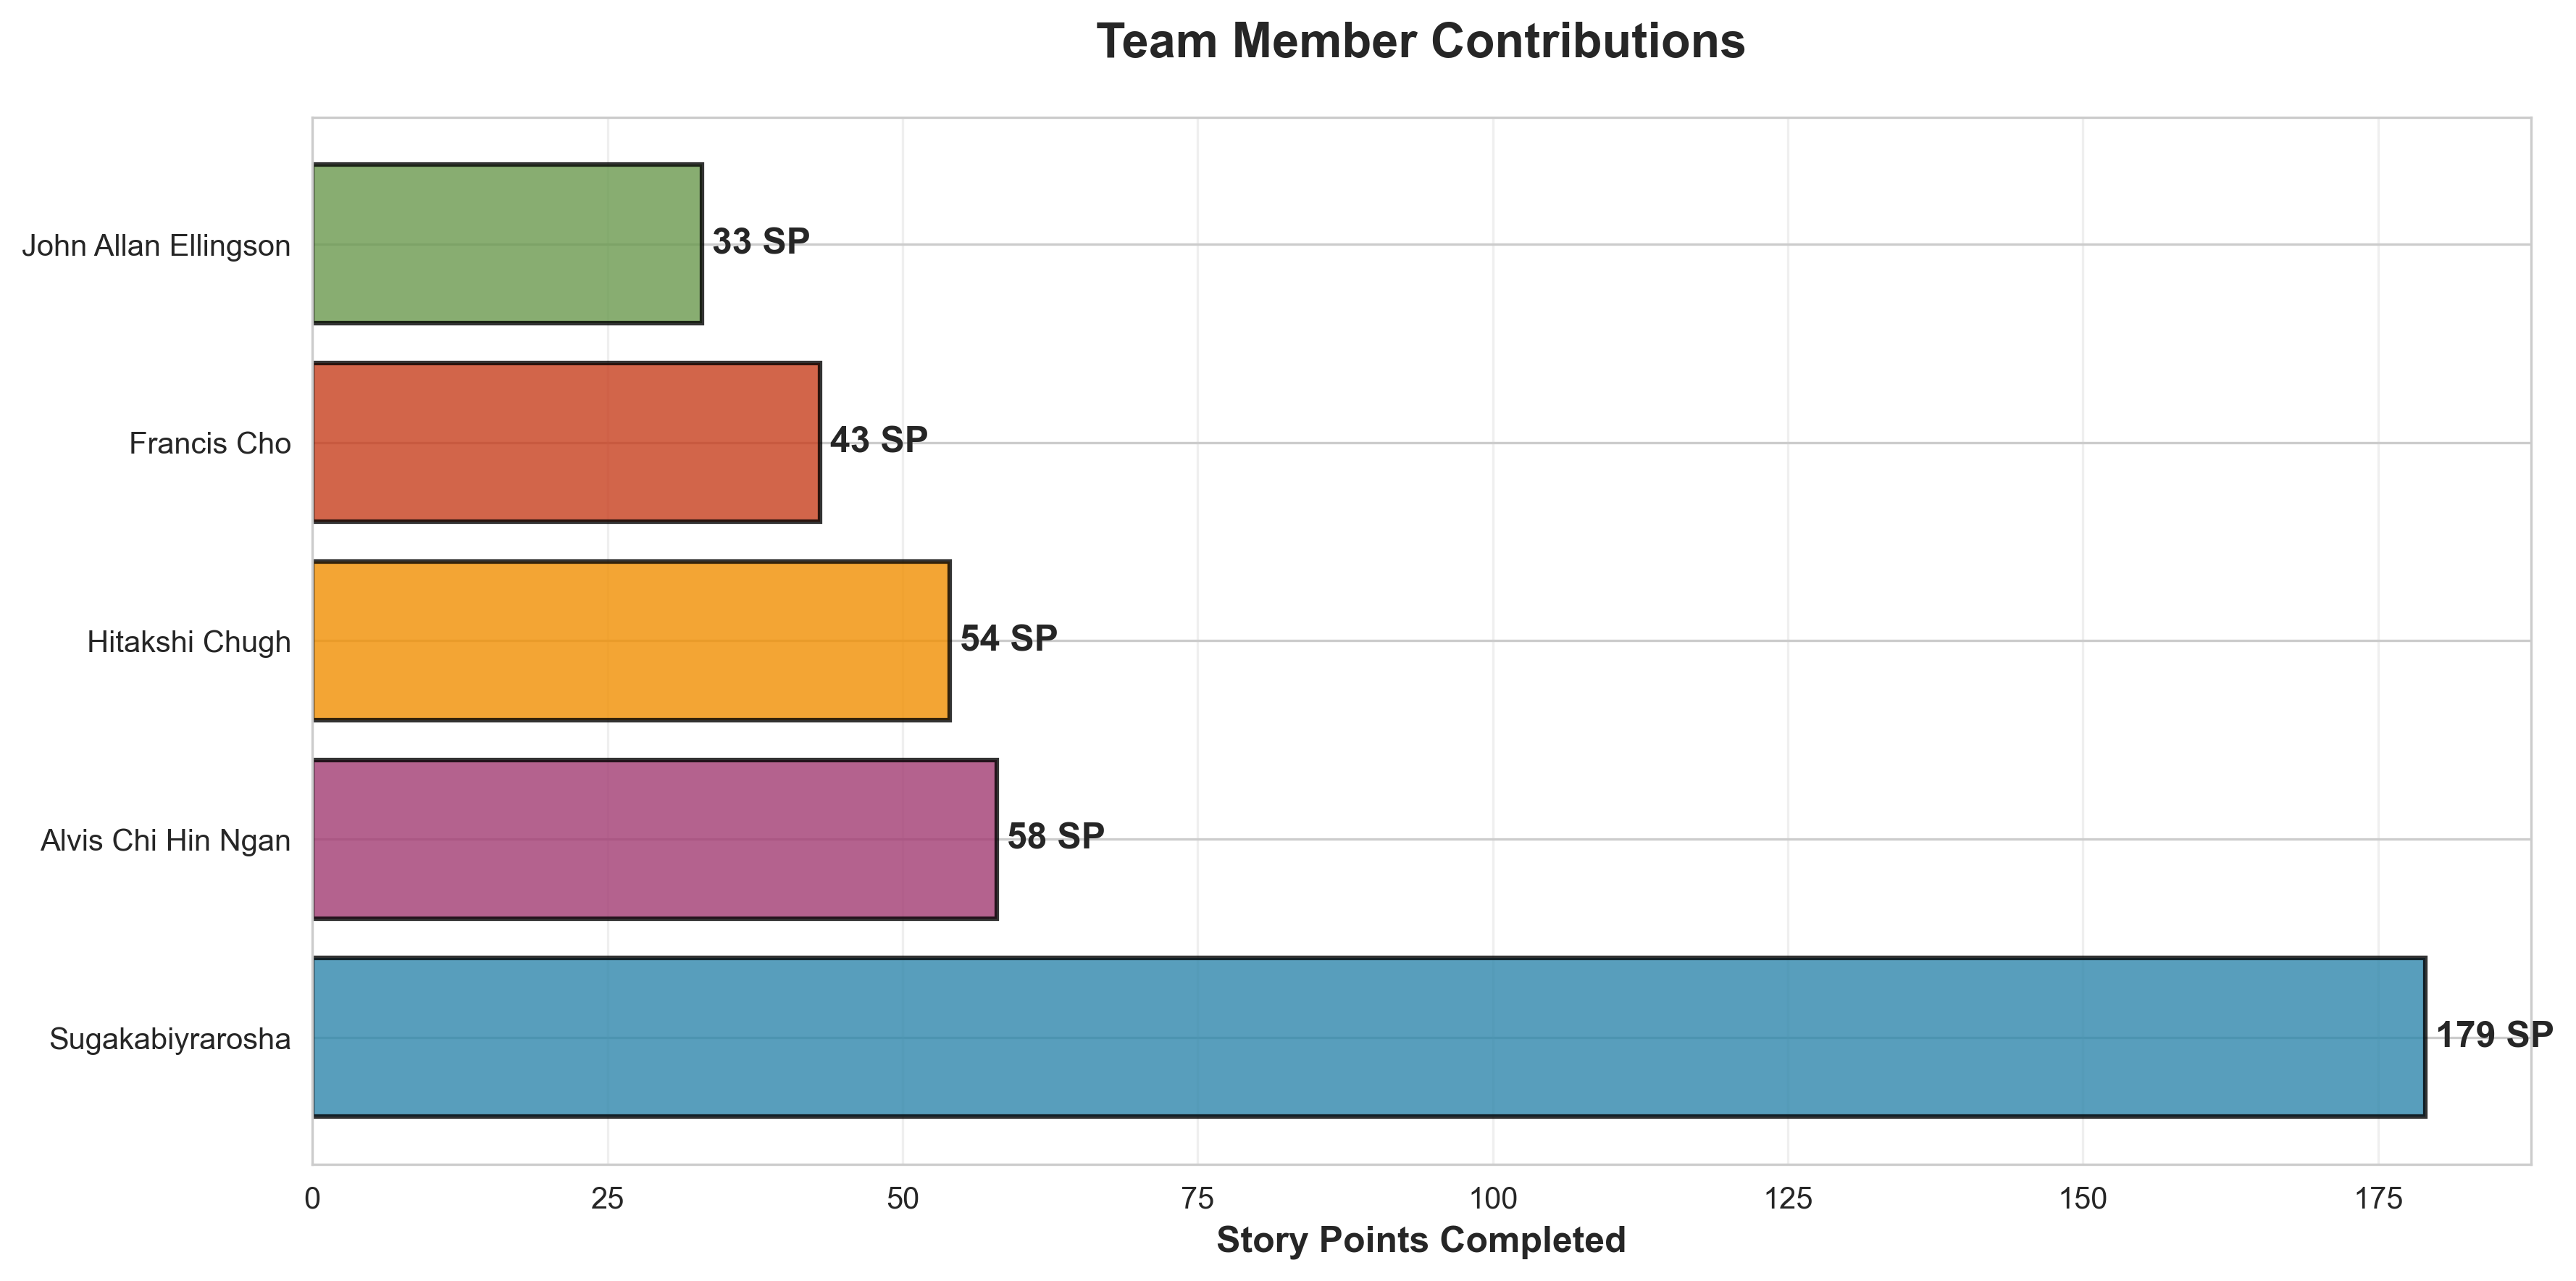
\includegraphics[width=0.9\textwidth]{temp/team_contributions.png}
\caption{Team Contributions Chart: Visualization of individual team member contributions and work distribution across the project.}
\label{fig:team_contributions_chart}
\end{figure}

\subsection{Sprint Retrospectives}

Each sprint concluded with a retrospective to identify what went well, challenges encountered, and action items for improvement. These retrospectives were instrumental in adapting the development process and improving team efficiency.

\textbf{Sprint 1 Retrospective:}
\begin{itemize}
    \item \textbf{What went well:} Successfully finalized project idea, explored datasets, established clear project structure, CNN baseline provided good starting point
    \item \textbf{Challenges:} Dataset format conversion complexity, initial environment setup coordination
    \item \textbf{Action Items:} Standardize data loading pipeline, improve documentation for dataset formats
\end{itemize}

\textbf{Sprint 2 Retrospective:}
\begin{itemize}
    \item \textbf{What went well:} Successfully implemented all four detection architectures, SAM fine-tuning improved segmentation, model comparison revealed performance differences, clustering approach identified stable parking locations
    \item \textbf{Challenges:} DETR training required significant computational resources, hyperparameter tuning was time-consuming, model evaluation metrics needed standardization, SAM fine-tuning required careful prompt engineering
    \item \textbf{Action Items:} Create standardized evaluation framework, document hyperparameter configurations, plan for Phase 2 improvements with augmentation
\end{itemize}

\textbf{Sprint 3 Retrospective:}
\begin{itemize}
    \item \textbf{What went well:} Data augmentation significantly improved model robustness, hyperparameter tuning found optimal configurations, all models showed improved performance, FastAPI provided excellent API framework, model loader abstraction simplified deployment, Docker containerization worked smoothly, team collaboration on report was effective
    \item \textbf{Challenges:} Hyperparameter tuning was computationally expensive, augmentation pipeline needed careful validation, model comparison required extensive testing, report writing required coordination across team, tight timeline for final sprint
    \item \textbf{Action Items:} Document optimal hyperparameters for each model, create augmentation validation pipeline, implement model caching for production, add API monitoring
\end{itemize}

\subsection{Key Achievements}

The agile methodology enabled the team to achieve:

\begin{enumerate}
    \item \textbf{Rapid Development:} Completed 118 story points in 3 weeks with 100\% completion rate
    \item \textbf{Comprehensive Model Implementation:} Successfully implemented 5 different model architectures (CNN, SSD, Faster R-CNN, DETR, YOLO) plus SAM fine-tuning
    \item \textbf{Performance Improvements:} Achieved significant performance improvements in Phase 2 through data augmentation and hyperparameter tuning
    \item \textbf{Production-Ready Deployment:} Developed complete API and deployment infrastructure
    \item \textbf{Effective Team Collaboration:} Balanced workload distribution and efficient resource sharing (GPU assistance)
    \item \textbf{Continuous Improvement:} Sprint retrospectives led to process improvements and better coordination
\end{enumerate}

\subsection{Lessons Learned}

The agile development process provided several key insights:

\begin{enumerate}
    \item \textbf{Early Baseline Establishment:} Establishing the CNN baseline early was crucial for comparison and setting expectations
    \item \textbf{Hyperparameter Tuning Impact:} Systematic hyperparameter tuning significantly improved model performance
    \item \textbf{Data Augmentation Value:} Data augmentation was key to model robustness and generalization
    \item \textbf{Unified Architecture:} Unified model loader simplified deployment and reduced code duplication
    \item \textbf{Team Collaboration:} Effective collaboration was essential for meeting tight timelines
    \item \textbf{Resource Sharing:} GPU resource sharing (Alvis) helped improve overall team efficiency
    \item \textbf{Documentation Importance:} Comprehensive documentation was essential for reproducibility and knowledge transfer
    \item \textbf{Agile Flexibility:} Agile methodology helped manage rapid development and changing requirements
\end{enumerate}

\section{Team Contributions}

\begin{table}[H]
\centering
\caption{Team Member Contributions}
\label{tab:contributions}
\begin{tabular}{@{}lp{10cm}@{}}
\toprule
\textbf{Member} & \textbf{Contributions} \\
\midrule
Francis Cho (Project Manager) & SAM model training, results analysis, report writing assistance, model comparison \\
Hitakshi Chugh (Scrum Master) & YOLO implementation, model training, results analysis, report writing assistance, model comparison \\
Sugakabiyrarosha & Dataset exploration, CNN baseline development, SSD, DETR model training, results analysis, hyperparameter tuning, main report writing, model comparison, local model deployment for SSD and Faster R-CNN \\
Alvis Chi Hin Ngan & Data augmentation, Faster R-CNN implementation, hyperparameter tuning, report writing assistance, GPU code running assistance for teammates \\
John Allan Ellingson & YOLO implementation and clustering pipeline, visualizations and statistical analyses, report writing assistance \\
\bottomrule
\end{tabular}
\end{table}

\section{References}

\begin{enumerate}
    \item Redmon, J., \& Farhadi, A. (2018). YOLOv3: An Incremental Improvement. \textit{arXiv preprint arXiv:1804.02767}.
    
    \item Liu, W., Anguelov, D., Erhan, D., Szegedy, C., Reed, S., Fu, C. Y., \& Berg, A. C. (2016). SSD: Single Shot MultiBox Detector. \textit{European conference on computer vision} (pp. 21-37).
    
    \item Ren, S., He, K., Girshick, R., \& Sun, J. (2015). Faster R-CNN: Towards Real-Time Object Detection with Region Proposal Networks. \textit{Advances in neural information processing systems}, 28.
    
    \item Carion, N., Massa, F., Synnaeve, G., Usunier, N., Kirillov, A., \& Zagoruyko, S. (2020). End-to-End Object Detection with Transformers. \textit{European conference on computer vision} (pp. 213-229).
    
    \item Roboflow. (2023). Parking Lot Dataset. \textit{Roboflow Universe}. Retrieved from \url{https://universe.roboflow.com}
    
    \item HuggingFace. (2023). Parking Space Detection Dataset. \textit{HuggingFace Datasets}. Retrieved from \url{https://huggingface.co/datasets/UniqueData/parking-space-detection-dataset}
    
    \item Almeida, P., Oliveira, L. S., Silva Jr, E., Britto Jr, A., \& Koerich, A. (2015). PKLot – A robust dataset for parking lot classification. \textit{Expert Systems with Applications}, 42(11), 4937-4949.
    
    \item PKLot Dataset. (2015). \textit{Universidade Federal do Paraná}. Retrieved from \url{https://web.inf.ufpr.br/vri/databases/parking-lot-database/}
    
    \item Ultralytics. (2023). YOLOv8 Documentation. \textit{Ultralytics}. Retrieved from \url{https://docs.ultralytics.com}
    
    \item PyTorch Team. (2023). Torchvision Models. \textit{PyTorch Documentation}. Retrieved from \url{https://pytorch.org/vision/stable/models.html}
\end{enumerate}

\end{document}

